\documentclass[12pt, a4paper]{article}
\usepackage[utf8]{inputenc}
\usepackage{amsmath}
\usepackage{amssymb}
\usepackage{natbib}
\usepackage{mathtools}
\usepackage{titling}
\usepackage[hidelinks]{hyperref}
\usepackage{booktabs}
\usepackage{float}
\usepackage{pbox}
\usepackage{adjustbox}
\usepackage{MnSymbol}
\usepackage{wasysym}
\usepackage{geometry}
\usepackage{ragged2e}
\usepackage[table]{xcolor} 
\usepackage[group-separator={,}, round-mode = places, round-precision = 2]{siunitx}

\usepackage{setspace}
%\doublespacing

\usepackage {tikz}
\usetikzlibrary{arrows}
\usetikzlibrary{shapes.misc, positioning, shapes.geometric}

\usepackage[font={it}, labelfont=bf]{caption}
\usepackage{graphicx}

\graphicspath{{images/}}

\author{Reid McIlroy-Young}
\title{Masters in Computational Social Science}
\date{May 1, 2018}

\setcounter{tocdepth}{2}

\begin{document}
\pagenumbering{gobble}
\maketitle
\tableofcontents
\newpage
\listoffigures
\listoftables
\newpage
\doublespacing
\setcounter{page}{1}
\pagenumbering{arabic}


\section{Introduction}

The mass proliferation of micro computers that began last century has had, and continues to have an incredible impact on society \citep{weizenbaum1972impact}, the economy \citep{gordon2000does} and information distribution \citep{berners2010world}. The access to computers -- the scale, quality and depth of data they provide -- has also had major effects on science \citep{lazer2009life}; but analysis has been primarily focused on either the macro cultural effects \citep{pfaffenberger1988social} or the economic usage \citep{landauer1995trouble} of computers.

By comparison, the usage of computers by scientists has been overlooked by researchers. The impact has spread, at different rates, throughout all the domains of science. The social sciences have been one of the last fields to be significantly affected, but this situation is likely to change this century \citep{watts2007twenty}. There are large datasets of medical, social and economic data generated by a complex web of automated systems whose implications we are not yet able to interpret at more than a surface level \citep{kossinets2006empirical} \citep{back2010emotional}, with many examples of even these surface level analyses failing \citep{lazer2014parable} \citep{kramer2014experimental}. One aspect of this `paradigm shift' that has received much less scrutiny is how the individual scientists are interacting with new computational tools. Are social scientists still able to do solid research with traditional with the traditional pre computational techniques or, or have computers changed?

One of the main methods for large scale analysis of the culture or structure of scientific work involves bibliometric techniques \citep{de2009bibliometrics} using large standard datasets tracing citations  between many articles \citep[e.g.][]{Boyack2005, borner2010atlas, borner2015atlas, sugimoto2013global, shi2015weaving, evans_meta, skupin2013visualizing}. These datasets have generally lacked information about the computational aspects of the works they contain. For  example the  Clarivate Analytics Web of Science (WOS) does not have any structured  metadata on the computational methods used by the publications in the database, such as the source code \citep{mkdocs}, and as such, research into this dimension is non-trivial. Nevertheless, recent developments in natural language processing (NLP) have shown that complex concepts can often be extracted reliably from text, providing a pathway to conducting research on computational methods in the literature \citep{evans2016machine} \citep{foster2015tradition}.

Large scale surveys of social scientists to determine computational usage have not been done, although much has been hypothesized regarding how computers or other computationally derived methods will revolutionize science \citep[e.g.][]{de1997computer, anderson2008end,  provost2013data, john2014big}. Moreover,  even quantitative  surveys  of  the  literature  have  not been  done. We can infer from the proliferation of new computational journals, such as the \textit{Journal of Computational Social Science}, the first issue of which published in January 2018, that there is a demand for computational knowledge and techniques within some  domains  of  social science,although its extent and means of spreading is not well characterized. This paper aims to begin to correct this lack of solid knowledge regarding computational approaches in social  science.  Once the usages of computation can be identified, there is a large number of existing frameworks from which the diffusion \citep{griliches1960hybrid}, spread \citep{padgett1993robust} and innovation \citep{foster2015tradition} of computational methods can be viewed.

In this paper, I am using a bidirectional Long Short Term Memory (LSTM) based classifier \cite{graves2005framewise}, which that I have been developing, for extract useful classifications with only partially or loosely classified data. The specific task is to identify the description of computational style, techniques, master, and approaches in journal articles, talks and other publications outside of the explicitly computational publications, conferences, or other sources. This paper seeks to both quantify the level of computational usage across publications in the social sciences and consider their implications.


\section{Methodology}

\subsection{Data}

The source of data used for this analysis is the Web of Science (WOS) database hosted by  \textit{Knowledge Lab}, a research group at the University of Chicago focused on developing  a  science  of  science \citep{chu2018too} with  large-scale publication resources. The Web of Science is owned by \textit{Thompson Reuters} until 2016, when it transferred to \textit{Clarivate Analytics}, who now maintains it \citep{clarivate}. Our  subset contains metadata from the most cited scientific and  social scientific publications from 1960 to 2015, with newer records being more complete. The data used are a subset of this larger collection, more specifically, the \num{1457418} publications with a Social Science subject classification from 2005 to 2015. The classifications of the publications are derived from the journals or conferences (hereafter called source) from which publications are drawn \citep{kottawos}. These  classifications  were grouped into six broad subjects (e.g. Natural Sciences, Social Sciences), each of which contain multiple subject categories (e.g. Cultural Studies or Ergonomics). Each source has up to three subject categories, which are assigned manually by WOS annotators and there could be many combinations  of 	subject classes that map to the same broad topic \citep{efremenkova2016comparison}. The classification  of  each  source  can  then  be  propagated to their publications, and thus I can assign a publication to one or more disciplines and sub-disciplines within a well defined hierarchy \citep{wossubjects}. A summary of the data is shown in Table \ref{sum_1}. Appendix \ref{app_tags} contains the complete list of tags used along with their subjects.

To derive information about the computational nature of soical science
publications, the \num{11115} sources from 2005 to 2017 containing explicitly computational subjects in the `Computer and information sciences' sub-discipline were intersected with the journals in the social sciences, yeilding \num{782} sources containing \num{106680} social science publications that are explicitly computational in nature. Table \ref{sum_comp} provides the breakdown according to subject, where the percentage of explicitly computational works notably varies by a massive factor of \num{50}, from \num{0.77}\% in Law to \num{38}\% in Media and Communication. 

In addition to the subject tags, the paper abstracts, titles, authors, publication month, publication year, and unique identification number (\textit{WOS ID}) were also gathered and used later in the analysis.

I also employed an additional dataset to help disaggregate computational features from WOS publications, the Stack Exchange Data Dump. This is a collection of user created technical question-answer data from the \href{http://stackexchange.com/}{Stack Exchange network}, hosted by the \href{https://archive.org/details/stackexchange}{Internet Archive} under a creative commons attribution share alike 3.0 license \citep{StackExchange}. The Stack Exchange network is a large collection of question and answer websites divided by category. In this case, the Stack Overflow (for general programming questions), Economics and Psychology \& Neuroscience Stack Exchange sites are of interest.From the Stack Exchange data dump, I used the user generated tags -- between one and three -- assigned by highly ranked community members.

\begin{table}[h]
	\centering
	\begin{adjustbox}{center}
		\begin{tabular}{lrrrl}
			\toprule
			{} &  \pbox{20cm}{Number of \\Publications}  &  \pbox{20cm}{Number of\\Sources}&  \pbox{20cm}{Number of \\Subjects} &   \pbox{20cm}{Example Subject\\Categories} \\
			\midrule
			Economics and Business  &            \num{459992} &              \num{2363} &                  \num{6} &            Business \\
			Psychology              &            \num{366313} &              \num{1017} &                 \num{11} &          Ergonomics \\
			Educational Sciences    &            \num{168342} &              \num{1009} &                  \num{3} &  Education, Special \\
			Sociology               &            \num{136894} &               \num{777} &                  \num{9} &           Sociology \\
			Political Science       &             \num{95920} &               \num{609} &                  \num{3} &   Political Science \\
			Other Social Sciences   &             \num{83611} &               \num{571} &                  \num{4} &       Asian Studies \\
			Media and Communication &             \num{63625} &               \num{518} &                  \num{2} &       Communication \\
			Law                     &             \num{40829} &               \num{295} &                  \num{2} &                 Law \\
			\midrule
			Full Data set           &           \num{1457418} &              \num{6893} &                 \num{46} &                     \\
			\bottomrule
		\end{tabular}
	\end{adjustbox}
	\caption{Summary of the subjects of WOS data. Note that publications can have multiple subjects, thus the final row is not a sum of the rows above.}\label{sum_1}
\end{table}

\begin{table}[h]
	\centering
	\begin{adjustbox}{center}
		\begin{tabular}{lrrl}
			\toprule
			{} &  \pbox{20cm}{Computational\\ Publications} &  \pbox{20cm}{Percentage\\Explicitly Computational} &  \pbox{20cm}{Example of Explicitly\\Computational Source} \\
			\midrule
			Economics And Business  &           \num{60602} &        \num{13.174577} &    Decision Support Systems \\
			Psychology              &            \num{5364} &         \num{1.464321} &  Interacting With Computers \\
			Educational Sciences    &           \num{17988} &        \num{10.685390} &       Computers \& Education \\
			Sociology               &            \num{3975} &         \num{2.903707} &       Persuasive Technology \\
			Political Science       &            \num{1815} &         \num{1.892202} &       Electronic Government \\
			Other Social Sciences   &            \num{2829} &         \num{3.383526} &           Adaptive Behavior \\
			Media And Communication &           \num{24798} &        \num{38.975246} &              Scientometrics \\
			Law                     &             \num{313} &         \num{0.766612} &    Law And The Semantic Web \\
			\midrule
			Full Data Set           &          \num{106680} &         \num{7.319794} &   \\
			\bottomrule
		\end{tabular}
	\end{adjustbox}
	\caption{Distribution of explicitly computational publications, note publications can have multiple subjects, thus the final row is not a sum}\label{sum_comp}
\end{table}


\subsection{Preprocessing}

In the WOS data, the publication year and month fields are provided as integers, so they required no preprocessing. Meanwhile, the other fields are all UTF-8 encoded raw texts, and I first tokenized both the title and the abstract by separating the words into separate strings. Then I used these texts to word embeddings. The tokenizing was done with the \textit{Natural Language Toolkit}'s (\textit{NLTK}) \citep{bird2006nltk} English language tokenizers, and more specifically, sentence tokenizing was done with the Punkt system \citep{kiss2006unsupervised} and the words tokenized with a collection of regular expressions derived from the Penn Treebank \citep{marcus1993building}. The other fields were treated as raw texts, without any additional transformations.

The final step in preparing the data for the neural network was constructing the word embeddings. A word embedding is a mapping from a collection of words to a collections of vectors in a high dimensional vector space with similar words closer together in the space \citep{wordembeding}. I used the \textit{Word2Vec} method \citep{mikolov2013efficient} implemented in \textit{gensim} \citep{rehurek_lrec}. \textit{Word2Vec} gives word vectors whose dimensions can be interpreted as a collection of semantic directions. For example, one direction could be the masculine-feminine dimension of the word while another could be the `computationalness' of the word \citep{bolukbasi2016man}. This relationship is derives from the neural auto-encoder used to perform the embedding as an approximation of SVD matrix factorization with words as rows and word contexts or windows as columns \citep{levy2014neural} that minimizes the point-wise mutual information, thus the space has many of the properties of a Euclidean Hilbert space. Unfortunately, determining the meaning of any one derived dimensions is impossible in practice, due to their number (in this case, 200 dimensions) and their non-linear relationships (the masculine-feminine direction, if it exists in the particular embedding, is a weighted combination of all 200 basis directions and is likely not orthogonal to `computationalness'). However, the embedding is still very useful as it assigns similar words with similar vectors and makes their divergences depend on their difference in meanings, e.g. king and queen diverge in similar ways to man and woman. The word embeddings act as a foundation for the deep neural network to build on and are the standard first step \citep{deep_learning_chapter12} as it converts variable length strings into fixed length vectors. For all embeddings, hierarchical softmax was used with a window size of five, 200 dimensional output, five iterations and no removal of words for any reason. This configuration should allow for infrequent words to be embedded nearly optimally  \citep{rehurek_lrec}, but there is also likely room for improvement.

An alternative to an auto-encoder is a one-hot vector representation where each word is a dimension of the input vector and all but one of the values is zero, with the non-zero element (usually equal to one) corresponding to the selected word's dimension. This method greatly increases the size of the first layer as in this case there are \num{11430321} unique words in the combined corpus, and it means that the RNN (Recurrent Neural Network) has to learn the meaning of each word separately as their location in the vector space provides no additional information. Thus, these methods are most commonly used for much simpler inputs, e.g. character level tasks \citep{rodriguez1999recurrent}.
 
 \subsection{Model Selection}\label{ness}
 
 Before undertaking the usage of a complex model such as that outlined above, it is worth considering the alternatives. There are many other ways to classify texts. A Naive Bayes model would generally be the first choice \citep{mccallum1998comparison}, while a K-nearest, SVM, ensemble or logit methods could also work. Unfortunately, none of these models were able to obtain anything better than random guessing, and most of them performed worse than random guessing when a pilot study was performed. The Naive Bayes model was the best performer, arriving at nearly $95\%$ accuracy on the training data, but when applied to the holdout set, it was worse than random guessing. This problem of over-fitting or for some models, always guessing negative, was present in all these models. Thus a model with a more nuanced understanding of language, such as a neural network, is required.
  
 \subsection{Model Description}

The classification of the publications was done with two separate, two layer bidirectional \citep{graves2013hybrid} Long Short Term Memory (LSTM) \citep{Hochreiter:1997:LSM:1246443.1246450} Recurrent Neural Networks (RNNs), with the LSTM implementation used is \textit{NVIDIA}'s \textit{cuDNN} \citep{chetlur2014cudnn}, see Figure \ref{lstm} for an illustration. LSTM cells are a variant of RNN cells, which work by taking in two vectors, the input vector (in this case, the word2vec vector of a word) and the recurrent vector which is initially all zeros. These two vectors are appended together to form a single input which is fed to a single layer neural network whose output layer has two components, the required output (in this case, the classification) and an output recurrent vector having the same size as the input recurrent vector. The output recurrent vector is then fed to the cell along with the next item in the sequence, thus giving a stateful component to the next output. Unfortunately, the memory of the cell tends to have short life span \citep{greff2017lstm} as every new input is combined with the memory vector. The LSTM architecture solves this by adding a second output vector, the blue lines in Figure \ref{lstm}. This second vector acts indirectly on the input and is in turn indirectly modified, via the peepholes, by the LSTM cell in each cycle. This configuration means that the \textit{long term} memory vector is modified much less by each input and thus retains more of the history. The weights of the cell are trained by backpropagation\citep{pytorch} just like most other neural network architectures, and the specifics of which have been thoroughly explored\citep{riedmiller1993direct}.

\begin{figure}[ht]
	\centering
	\begin{adjustbox}{center}
		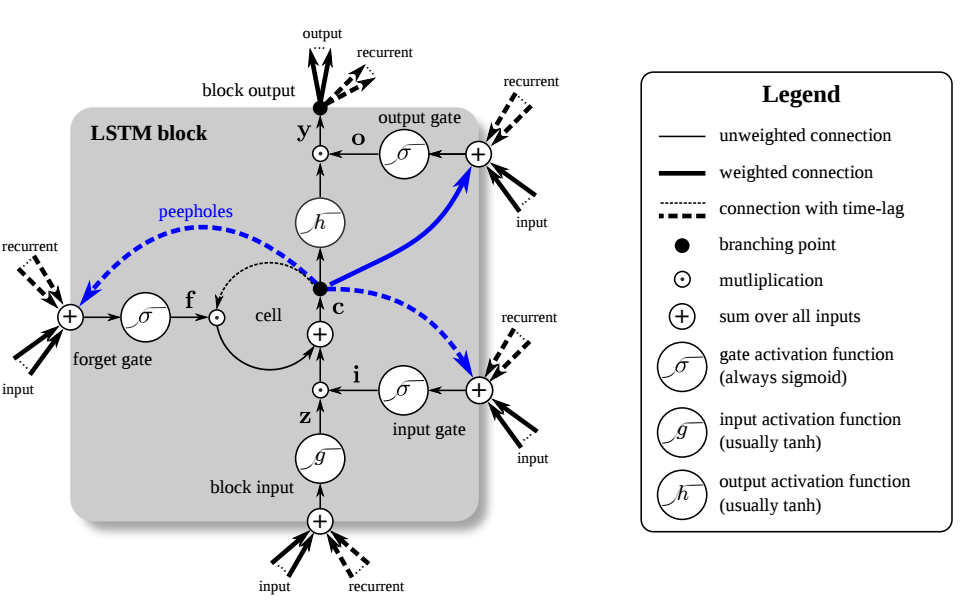
\includegraphics[width=1\textwidth]{LSTM.png}
	\end{adjustbox}
	\caption{Illustration of LSTM cell as implemented by \textit{NVIDIA}\\Image by Klaus Greff and colleagues as published in LSTM: A Search Space Odyssey \citep{greff2017lstm}}\label{lstm}
\end{figure}

To create the classifier used in this paper, 16 LSTM cells were used, their arrangement is shown in Figure \ref{rnn}, which shows the network's structure and the flow of data through the model. Starting from the bottom, the abstract and the title are provided as raw text, which then go through the two preprocessing steps, tokenizing and embedding, and then the result of which is that each word becomes a vector $\vec{x}_t = \begin{bmatrix}0&.2&0&\dots&.3&0\end{bmatrix}^T$. The process is identical, modulus weights, for the title and abstract, and for this example we will consider only the title. A word's vector is fed to the first forward layer ($h_t^1$) of the RNN, which applies the non-linear transforms described above, before finally outputting three $128$ dimensional vectors (\textit{long term}, \textit{short term} and an output vector). The output is then fed to the next layer ($h_t^1 \rightarrow h^2_t$) while the memory vectors are given back to the cell along with the next word vector ($h_t^1 \rightarrow h^1_{t+1}$). The next layer repeats the process with the output ignored, until the final word is provided. These ignored outputs can be of use and will be discussed. Simultaneously, the last word is provided to the first reverse layer  ($g^1_t$) where the same process as the forward layer takes place, the output is fed up the network ($g_t^1 \rightarrow g^2_t$) while the memory vectors go to the next (previous word in the text) word  ($g_t^1 \rightarrow g^2_{t+1}$). The final output vectors ($128$ dimensional) from the final word in the title in the forward direction along with the final word from the backward direction are appended to each other to create one vector ($\oplus$), a $256$ dimensional vector giving the module's `thoughts' on what was in the title. This vector is then combined with the output from the abstract and given to a final neural network ($u$) that looks at the two combined 512 dimensional vector and produces a single 2 dimensional vector ($\vec{y}$). The two dimensions provided are the log-odds of the publication \textit{not} being computational and the log-odds of the publication being computational.

When the neural network first runs on a publication, its weights, the parameters for the non-linear transforms, are randomly selected, so it's outputs are useless. Thus it has to be trained. To train the model, a training dataset is created and labelled with the correct outputs for each of the publications in the set. Then publications are randomly selected from the set to be fed through the network and to have the outputs compared to the expected outputs. Through the use of backpropagation \citep{werbos1982applications} (differentiating the output with respect to every parameter and every input), the given output and correct output are compared and the network's weights are updated to move future outputs more in line with the correct outputs. The networks are then tested for accuracy against a separate set of publications, the testing set, once an epoch (in this case, 500 training examples), to see if it is making accurate predictions.

\begin{figure}[H]
	\centering
	
	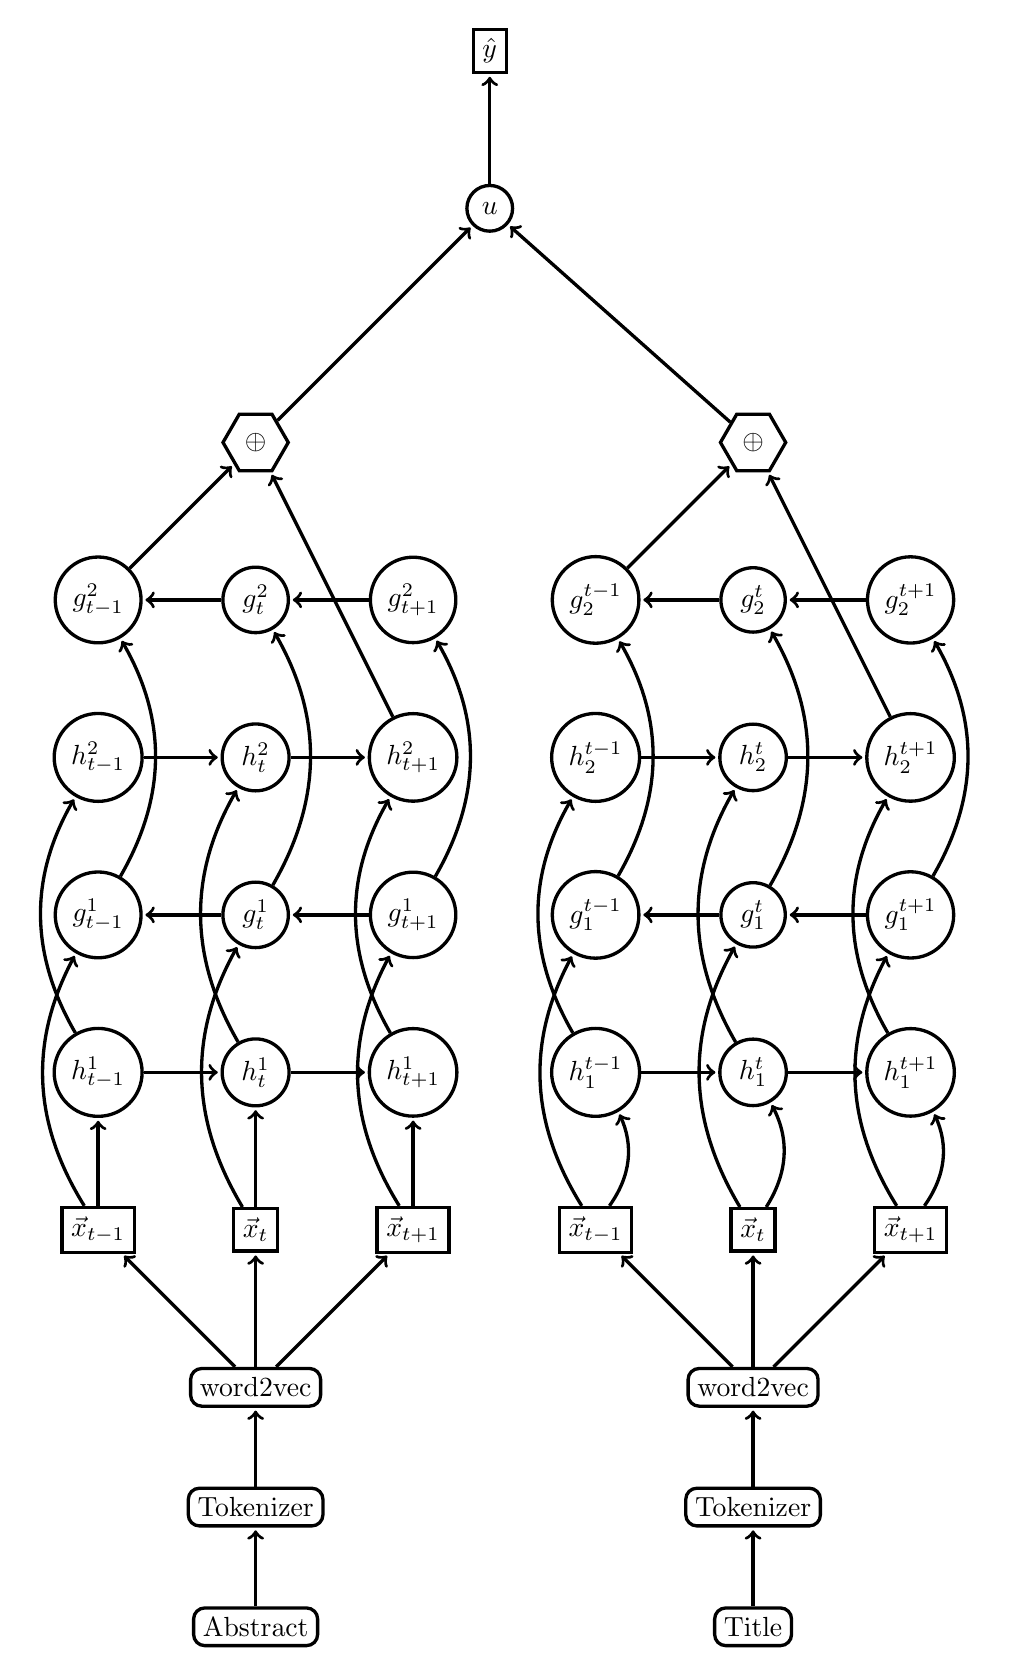
\begin{tikzpicture}[shorten >=1pt,auto,node distance=2cm, very thick]
	\node[draw, rounded corners] (1) {Abstract};
	\node[draw, rounded corners] (tokenizer) [above = 1cm of 1] {Tokenizer};
	\node[draw, rounded corners] (2) [above = 1cm of tokenizer] {word2vec};
	\node[draw] (3) [above of=2] {$\vec{x}_{t}$};
	\node[draw] (4) [left of =3] {$\vec{x}_{t-1}$};
	\node[draw] (5) [right of =3] {$\vec{x}_{t+1}$};
	
	\node[draw, circle] (h1) [above of=3] {$h_t^1$};
	\node[draw, circle] (h2) [above of=4] {$h_{t-1}^1$};
	\node[draw, circle] (h3) [above of=5] {$h_{t+1}^1$};
	
	\node[draw, circle] (g1) [above of=h1] {$g_t^1$};
	\node[draw, circle] (g2) [above of=h2] {$g_{t-1}^1$};
	\node[draw, circle] (g3) [above of=h3] {$g_{t+1}^1$};
	
	\node[draw, circle] (h12) [above of=g1] {$h_t^2$};
	\node[draw, circle] (h22) [above of=g2] {$h_{t-1}^2$};
	\node[draw, circle] (h32) [above of=g3] {$h_{t+1}^2$};
	
	\node[draw, circle] (g12) [above of=h12] {$g_t^2$};
	\node[draw, circle] (g22) [above of=h22] {$g_{t-1}^2$};
	\node[draw, circle] (g32) [above of=h32] {$g_{t+1}^2$};
	
	\node[draw, regular polygon, regular polygon sides=6] (L) [above of=g12] {$\oplus$};
	
	\node[draw, rounded corners] (1t) [right = 5cm of 1]{Title};
	\node[draw, rounded corners] (tokenizert) [above = 1cm of 1t] {Tokenizer};
	\node[draw, rounded corners] (2t) [above = 1cm of tokenizert] {word2vec};
	
	\node[draw] (3t) [above of=2t] {$\vec{x}_{t}$};
	\node[draw] (4t) [left of =3t] {$\vec{x}_{t-1}$};
	\node[draw] (5t) [right of =3t] {$\vec{x}_{t+1}$};
	
	\node[draw, circle] (h1t) [above of=3t] {$h^{ t}_1$};
	\node[draw, circle] (h2t) [above of=4t] {$h^{ t-1}_1$};
	\node[draw, circle] (h3t) [above of=5t] {$h^{t+1}_1$};
	
	\node[draw, circle] (g1t) [above of=h1t] {$g^{t}_1$};
	\node[draw, circle] (g2t) [above of=h2t] {$g^{t-1}_1$};
	\node[draw, circle] (g3t) [above of=h3t] {$g^{t+1}_1$};
	
	\node[draw, circle] (h1t2) [above of=g1t] {$h^{ t}_2$};
	\node[draw, circle] (h2t2) [above of=g2t] {$h^{ t-1}_2$};
	\node[draw, circle] (h3t2) [above of=g3t] {$h^{t+1}_2$};
	
	\node[draw, circle] (g1t2) [above of=h1t2] {$g^{t}_2$};
	\node[draw, circle] (g2t2) [above of=h2t2] {$g^{t-1}_2$};
	\node[draw, circle] (g3t2) [above of=h3t2] {$g^{t+1}_2$};
	
	
	\node[draw, regular polygon, regular polygon sides=6] (Lt) [above of=g1t2] {$\oplus$};
	\node[draw, circle] (u) [above right = 3.5cm of L]{$u$};
	\node[draw] (y) [above of = u]{$\hat{y}$};
	
	
	\draw[->] (L) -- (u);
	\draw[->] (Lt) -- (u);
	\draw[->] (u) -- (y);
	
	\draw[->] (1) -- (tokenizer);
	\draw[->] (tokenizer) -- (2);
	\draw[->] (2) -- (3);
	\draw[->] (2) -- (4);
	\draw[->] (2) -- (5);
	
	\draw[->] (3) -- (h1);
	\draw[->] (4) -- (h2);
	\draw[->] (5) -- (h3);
	\draw[->] (h2) -- (h1);
	\draw[->] (h1) -- (h3);
	
	\draw[->] (3)  edge[bend left] (g1);
	\draw[->] (4) edge[bend left] (g2);
	\draw[->] (5) edge[bend left] (g3);
	\draw[->] (g1) -- (g2);
	\draw[->] (g3) -- (g1);
	
	\draw[->] (h1)  edge[bend left] (h12);
	\draw[->] (h2) edge[bend left] (h22);
	\draw[->] (h3) edge[bend left] (h32);
	\draw[->] (h22) -- (h12);
	\draw[->] (h12) -- (h32);
	
	\draw[->] (g1)  edge[bend right] (g12);
	\draw[->] (g2) edge[bend right] (g22);
	\draw[->] (g3) edge[bend right] (g32);
	\draw[->] (g12) -- (g22);
	\draw[->] (g32) -- (g12);
	
	\draw[->] (g22) -- (L);
	\draw[->] (h32) -- (L);
	
	\draw[->] (1t) -- (tokenizert);
	\draw[->] (tokenizert) -- (2t);
	\draw[->] (2t) -- (3t);
	\draw[->] (2t) -- (4t);
	\draw[->] (2t) -- (5t);
	
	\draw[->] (3t) edge[bend right] (h1t);
	\draw[->] (4t) edge[bend right] (h2t);
	\draw[->] (5t) edge[bend right] (h3t);
	\draw[->] (h2t) -- (h1t);
	\draw[->] (h1t) -- (h3t);
	
	\draw[->] (3t)  edge[bend left] (g1t);
	\draw[->] (4t) edge[bend left] (g2t);
	\draw[->] (5t) edge[bend left] (g3t);
	\draw[->] (g1t) -- (g2t);
	\draw[->] (g3t) -- (g1t);
	
	\draw[->] (h1t)  edge[bend left] (h1t2);
	\draw[->] (h2t) edge[bend left] (h2t2);
	\draw[->] (h3t) edge[bend left] (h3t2);
	\draw[->] (h2t2) -- (h1t2);
	\draw[->] (h1t2) -- (h3t2);
	
	\draw[->] (g1t)  edge[bend right] (g1t2);
	\draw[->] (g2t) edge[bend right] (g2t2);
	\draw[->] (g3t) edge[bend right] (g3t2);
	\draw[->] (g1t2) -- (g2t2);
	\draw[->] (g3t2) -- (g1t2);
	
	\draw[->] (g2t2) -- (Lt);
	\draw[->] (h3t2) -- (Lt);
	\end{tikzpicture}
	\caption[Unfolded Model Graph]{Simplified recursive bidirectional Recursive NN (RNN) layout, LSTM connections were removed for clarity. Circles are NN layers, rectangles with curved corners are the preprocessing, hexagons are combined outputs from the RNN layers, and final output and inputs are indicated with squared corners.}\label{rnn}
\end{figure}


\section{Results}

\subsection{Training}

 Two separate approaches were tried for training the network, namely, using one network per subject and using one network for the complete dataset. Training the network proved to be more difficult than expected. Data gathering took many hours, limitations of the database made bibliographic data collection difficult, and data prepossessing was time consuming and took about two weeks on a high end laptop.  

\subsubsection{One Network Per Subject}

To reduce the word embedding run time, each subject was separated and the embeddings run independently, with \textit{Law} taking a few hours and \textit{Economics and Business} a couple days to complete. Since the embeddings are independent across subjects, each subject has to have a separate network trained for it.

To train the networks, all the explicitly computational records were combined with a random sample of non-explicit records of twice the size of the explicit set, except in \textit{Media And Communication} where the complete collection was used due to proliferation of computational journals. Then a holdout set of $10\%$ was removed to be used for cross validation.

The models were trained with stochastic gradient descent with the Adam optimizations \citep{collins2012advertiser} and a cross entropy loss. Equation \ref{cross_en} gives the exact formulation used \citep{pytorch}. During training, after every 500 updates to the model (1 epoch), the testing set error was checked. The preferred way to do this is with a loss function, in this case, the loss \citep{deeploss} was the cross-entropy of the expected output and the actual output . The cross-entropy can take any positive value, although less than 1 is expected after training. Using average loss to quantify the model's accuracy instead of the raw error rate is preferable as it is less jittery \citep{deeploss} and picks up small improvements (or deteriorations) that are missed with a binary successful/not successful. There are many other measures available, such as the area under the testing receiver operating characteristic curve or the $F_1$ score \citep{james2013introduction}, but those are more useful for tuning the model and many require additional computation.

\begin{align}\label{cross_en}
	loss(\boldsymbol{output}, \boldsymbol{expected}) = - \log \left(\frac{\exp(\boldsymbol{output} \cdot \boldsymbol{expected})}{\sum_j \exp (\boldsymbol{output}_j)}\right)
\end{align}

\begin{figure}[ht]
	\centering
	\begin{adjustbox}{center}
		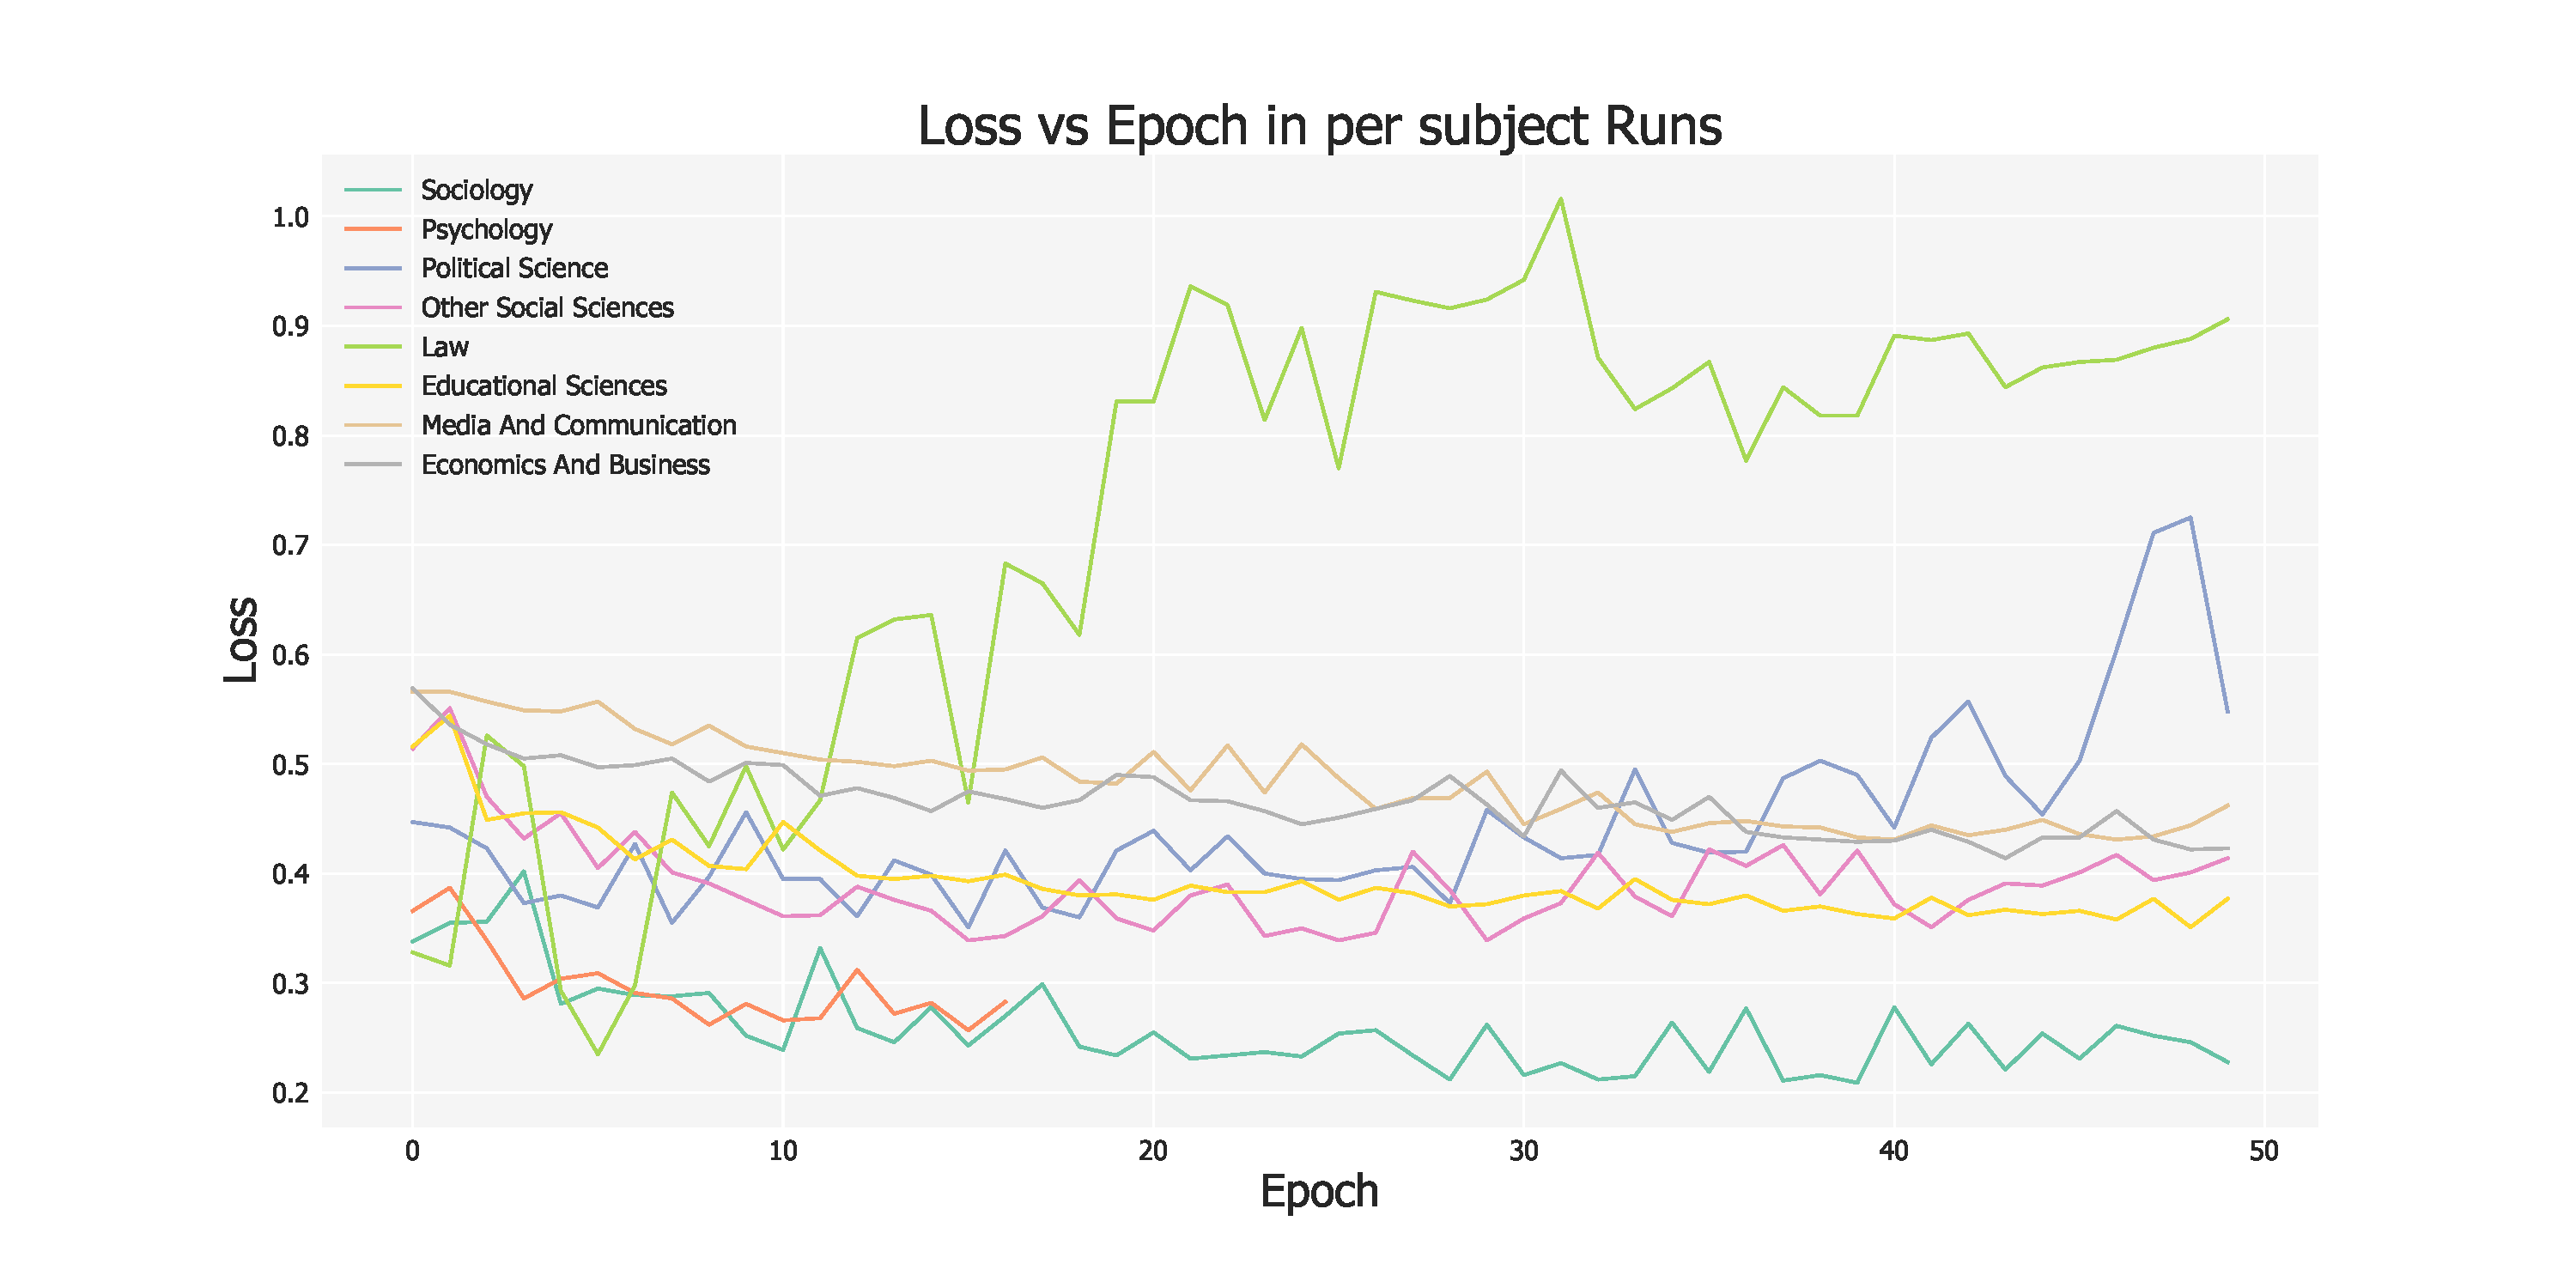
\includegraphics[width=1.3\textwidth]{loss_mixed}
	\end{adjustbox}
	\caption{Testing loss for all subject's models, across all epochs (1 epoch is 500 training exposures), note that some data for Psychology was lost}\label{loss}
\end{figure}

\begin{figure}[ht]
	\centering
	\begin{adjustbox}{center}
		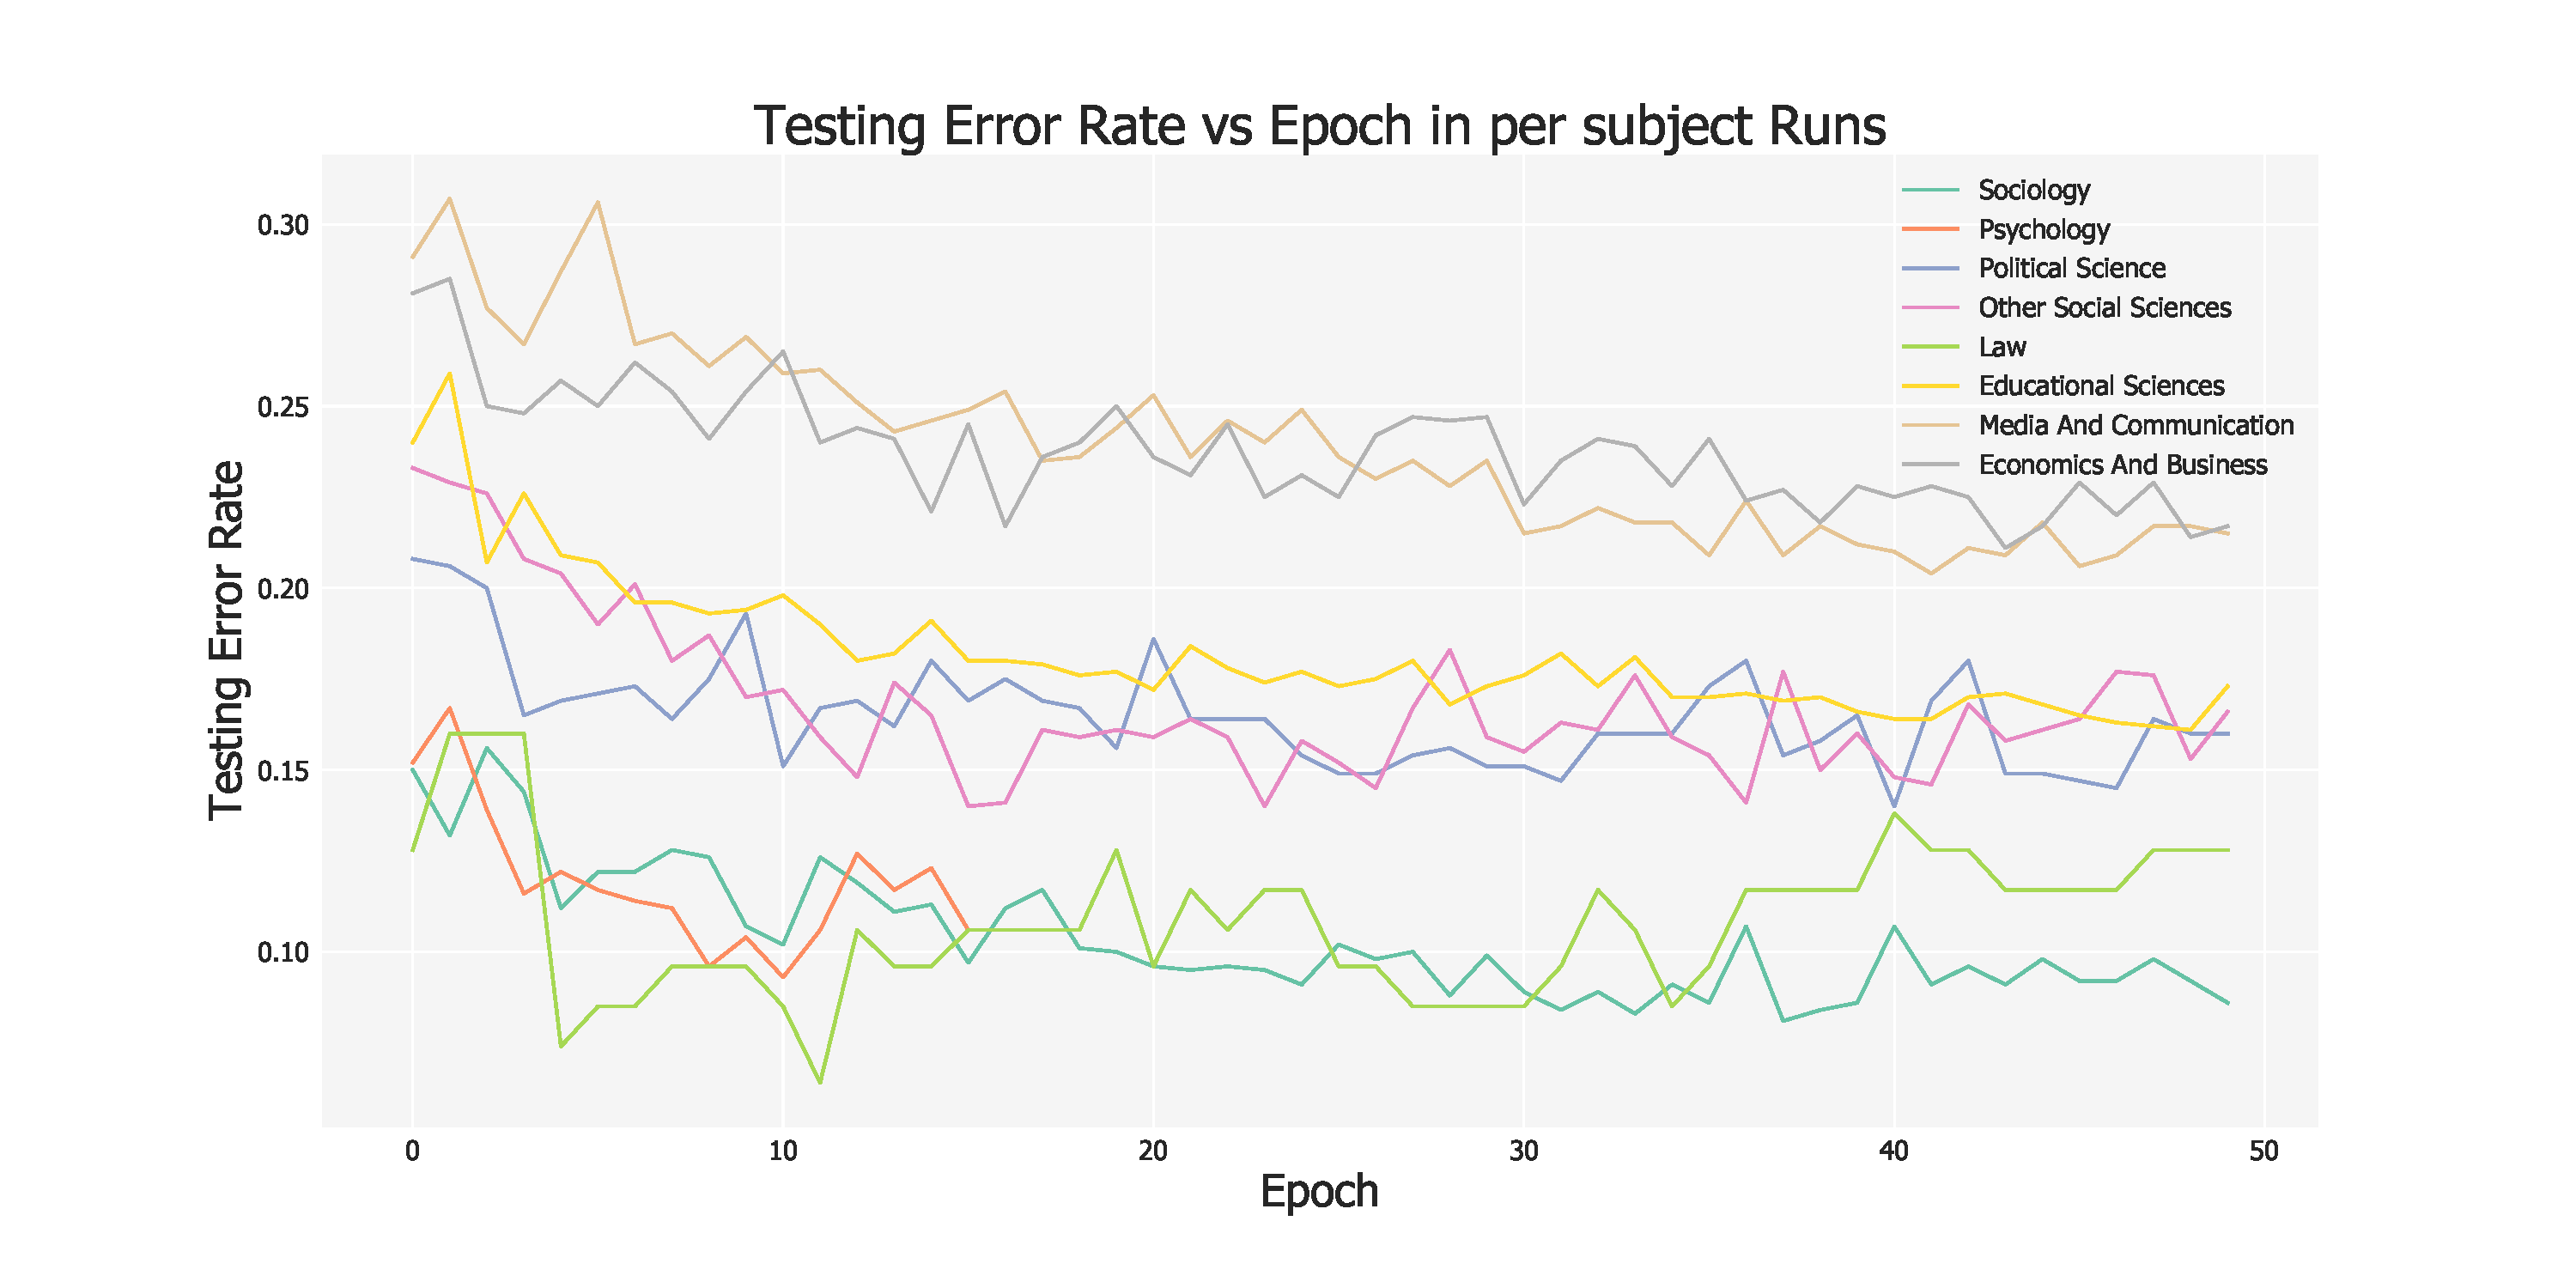
\includegraphics[width=1.3\textwidth]{err_mixed}
	\end{adjustbox}
	\caption{Testing error for all subject's models, across all epochs (1 epoch is 500 training exposures), note that some data for Psychology was lost}\label{err}
\end{figure}

\begin{table}[ht]
	\centering
	\begin{adjustbox}{center}
		\begin{tabular}{lrr}
			\toprule
			{} &  Testing Error &   Loss \\
			\midrule
			Economics And Business  &         \num{0.247} & \num{0.463} \\
			Psychology              &         \num{0.121} & \num{0.272} \\
			Educational Sciences    &         \num{0.173} & \num{0.372} \\
			Sociology               &         \num{0.099} & \num{0.262} \\
			Political Science       &         \num{0.151} & \num{0.458} \\
			Other Social Sciences   &         \num{0.159} & \num{0.339} \\
			Media And Communication &         \num{0.235} & \num{0.493} \\
			Law                     &         \num{0.085} & \num{0.924} \\
			\bottomrule
		\end{tabular}
	\end{adjustbox}
	\caption{The testing loss and error for each subject on the epoch used for the analysis}\label{final_loss}
\end{table}

Figure \ref{loss} shows the loss on the testing set across the epochs for each of subject's models. Notice the slow drop of \num{0.1} or so from epoch 0 to epoch 30, at which point they cease decreasing. The plot for \textit{Law}, is not representative of the model's accuracy and the jump is due more to the small testing set size (94) as a couple of examples being misclassified will cause a large jump. The loss shown for law, is not the first attempt. In the first run, it had the lowest loss and a testing error of 0 for most epochs, which is a sign of over-fitting more than of a quality model, so it was discarded. Over-fitting is a major concern when training neural networks \citep{james2013introduction} and the characteristic switch from nearly flat slope to positive slope is visible in some of the losses, most notably \textit{Political Science} and \textit{Other Social Sciences}.

To help avoid over-fitting, the testing error rates are also considered, with Figure \ref{err} showing them against epoch number. They are nosier than the loss, so they are a secondary consideration as discussed above. In the testing error, again, the errors tend to stabilize around epoch 30 , so epoch 30 was chosen to use for analysing the complete dataset, Figure \ref{final_loss} shows the final values of testing loss and testing error at this epoch. Also note that the error rate for \textit{Law} is quite low despite the high loss, this confirms the small dataset is causing anomalies in the loss.

\subsubsection{Complete}

Once the per subject networks had been trained and tested, training a model on the complete dataset could follow. A word embedding was created across the whole dataset, which took about a week running on a server. Then the explicitly computational records were identified and combined with twice their count of non-computational records and a $10\%$ testing holdout set was created. The model was initially tested on a small subset of the testing data, but at epoch 112, the test set was switched to random samples from the complete set to make sure over fitting was not occurring. The epoch size for this model is 2000 records as it took much longer to converge, and Adam based stochastic gradient descent was still used along with cross-entropy loss. 

Figure \ref{full_loss} shows the loss per epoch of the complete model. The model seems to have  stopped improving around epoch 250, which is \num{35000} more exposures than any of the simple subject networks, thus this was a much slower process taking days on a NVIDIA GeForce GT 750M with \num{2048} MB of RAM. The final model used for this analysis was from epoch 260 as that had particularity good testing error of \num{0.134} and loss of \num{0.316}. Compared to any of the per subject networks it is better than all but \textit{Sociology} and \textit{Law}. Of note is that there were \num{288646} records in the training set, while the model was exposed to \num{520000} records so the model saw each example on average only twice.


\begin{figure}[H]
	\centering
	\begin{adjustbox}{center}
		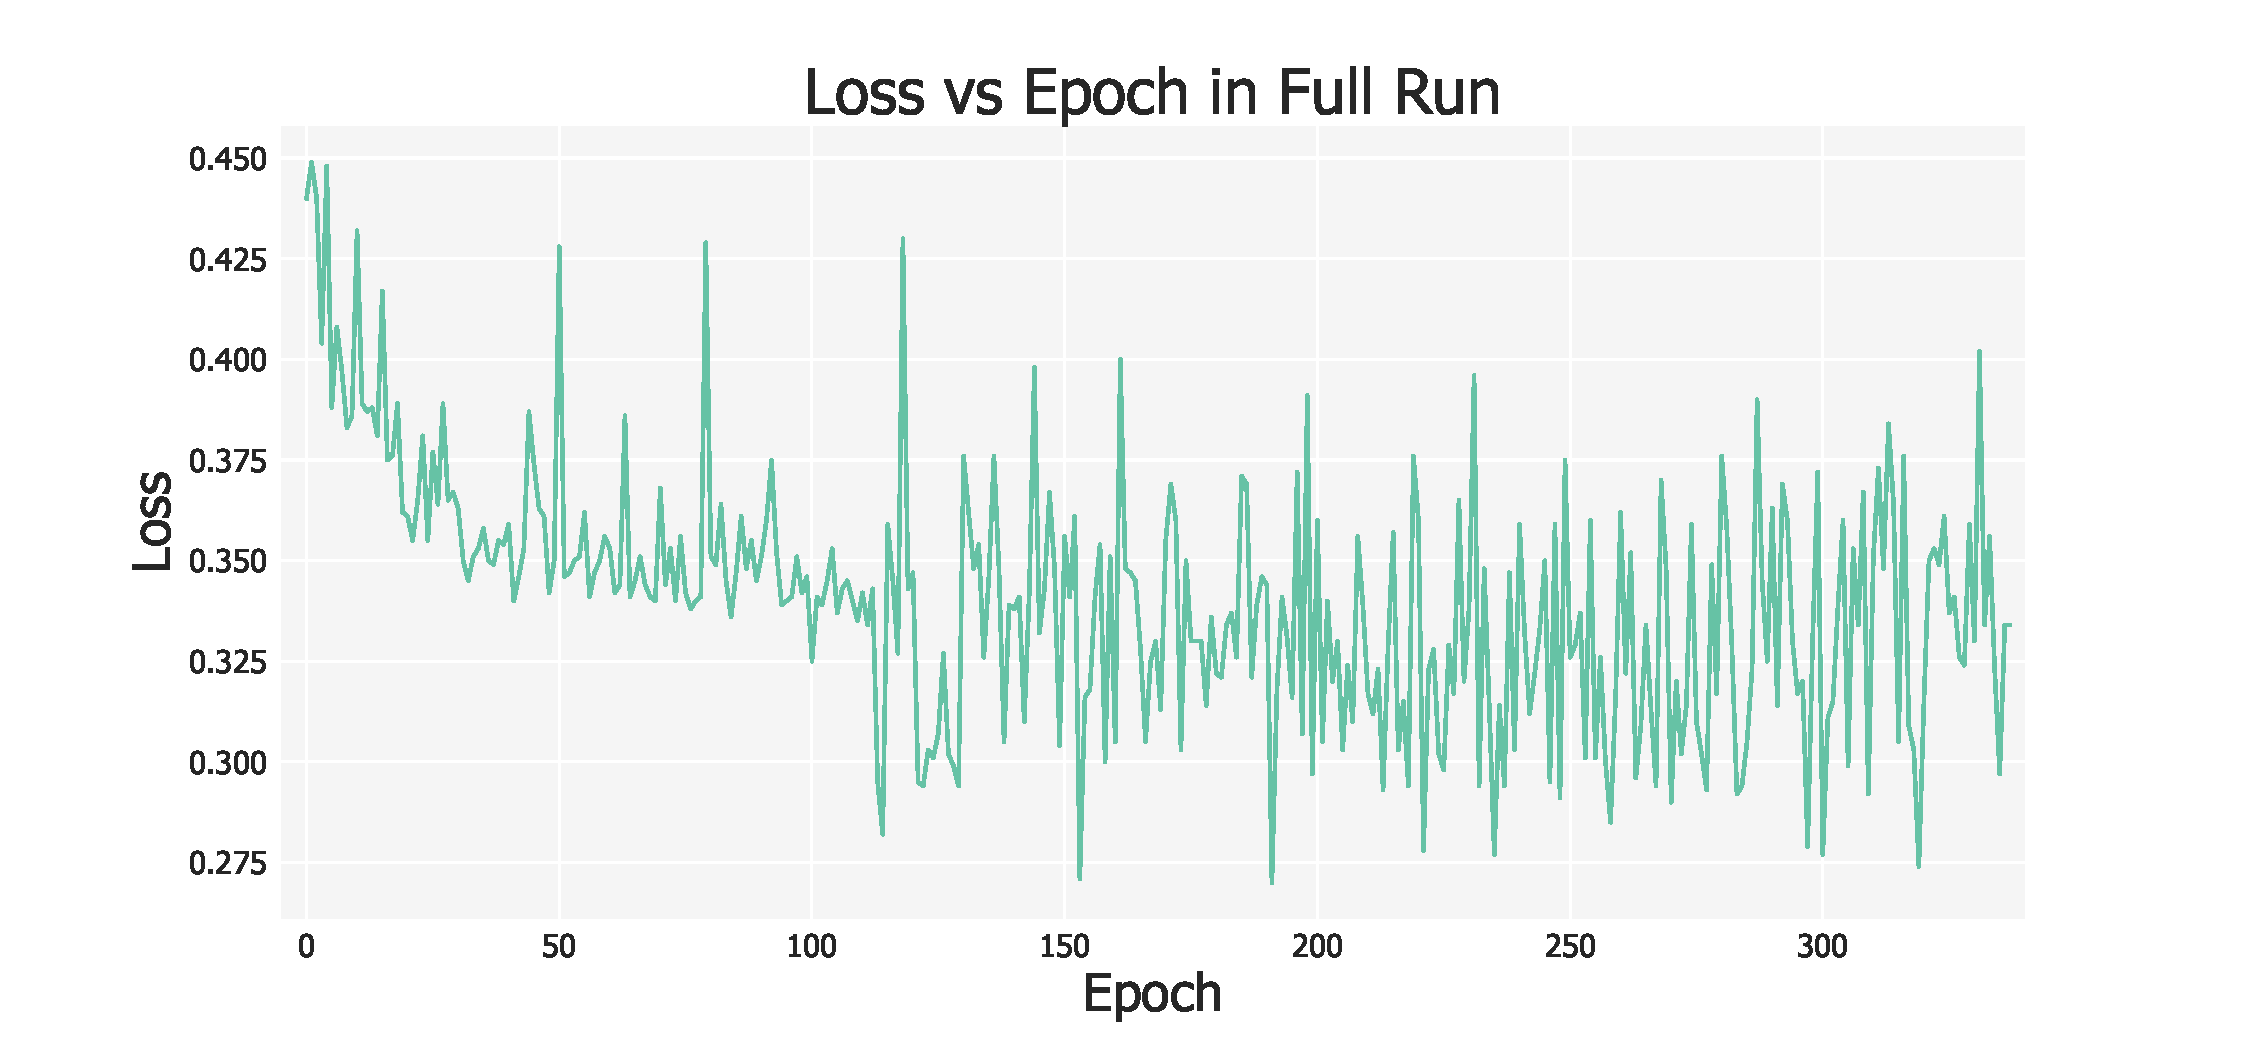
\includegraphics[width=1.3\textwidth]{full_loss}
	\end{adjustbox}
	\caption{Testing loss for all complete  model, across all epochs (1 epoch is 2000 training exposures), note that at epoch 112 the testing set was expanded}\label{full_loss}
\end{figure}

\begin{figure}[H]
	\centering
	\begin{adjustbox}{center}
		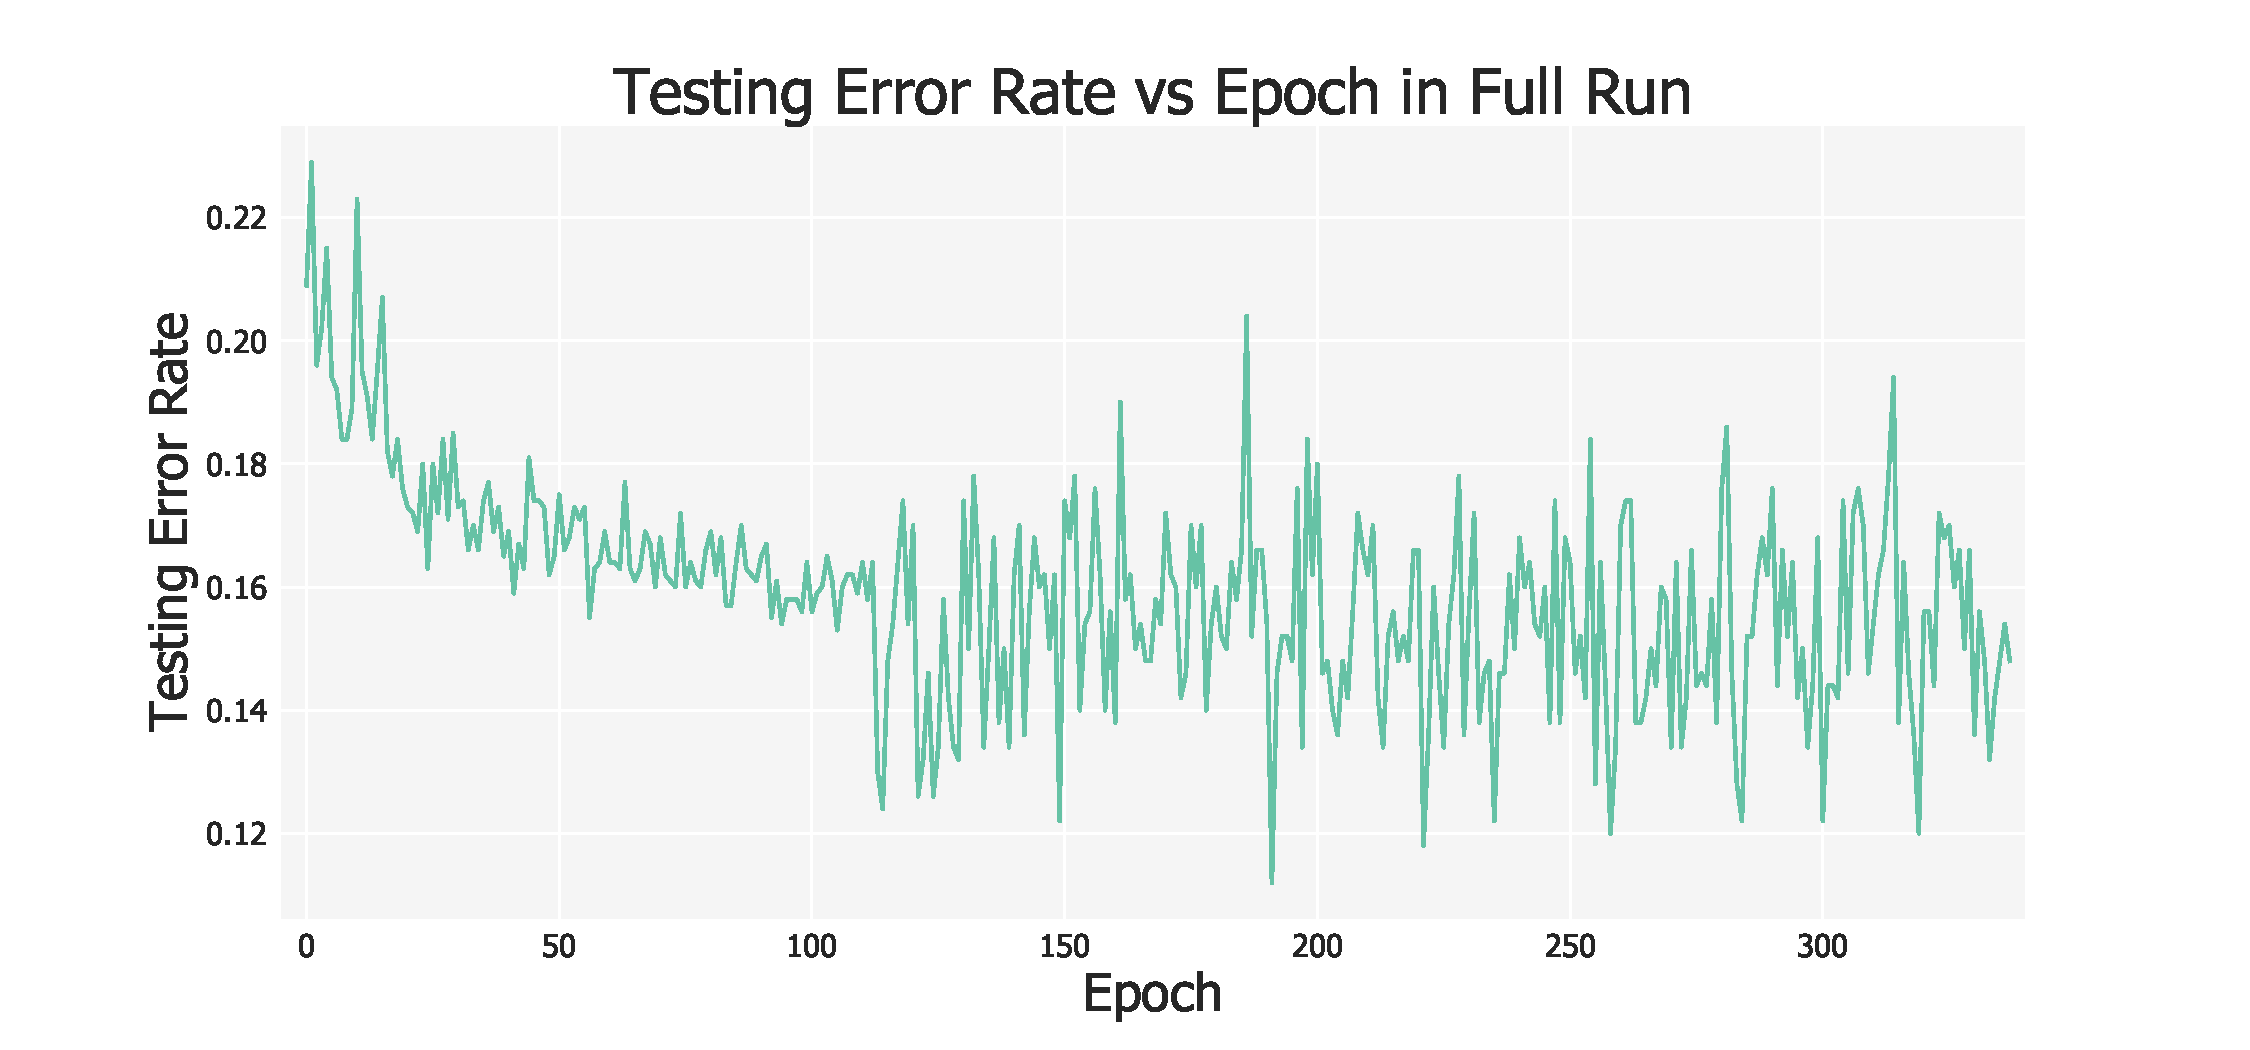
\includegraphics[width=1.3\textwidth]{full_testing_error_rate}
	\end{adjustbox}
	\caption{Testing error rate for all complete  model, across all epochs (1 epoch is 2000 training exposures), note that at epoch 112 the testing set was expanded}\label{full_testing_error_rate}
\end{figure}

\subsection{Word2Vec}

Before considering the results of the models, the validity of the foundations need to be tested. In particular the Word2Vec embedding space is worth some consideration. Using the tags from stack overflow, a vocabulary of key words can be constructed. Stack Overflow can be considered to be computational, and Economics and Psychology \& Neuroscience are two sets of keywords for non-computational subjects. There is a large bias in Stack Exchange towards computational topics as Stack Overflow was the first and largest site. Thus tags for Stack Overflow were trimmed to only those with over \num{10000} usages, while the other two sites are unfiltered. Then the tags found in the the Word2Vec embedding space were collected and their embeddings derived, the number of tags used are given in Table \ref{tags}. 

To visualize the distribution of tags, a dimension reduction is required. Principal component analysis was used to reduce the number of dimensions from 200 to 50, and then t-distributed stochastic neighbor embedding (t-SNE) \citep{maaten2008visualizing} was used to go from 50 to 2. This was done separately for each of the three site's tags, Figure \ref{tsne_indv} and together, Figure \ref{tsne_combined}, Appendix \ref{appendix_tsne} has larger versions of the individual plots. Upon examination, the tags are roughly clustered as expected, e.g. \texttt{mysql} is near \texttt{database} and \texttt{gdp} is near \texttt{inflation}. But when examined further, there are a few oddities. \texttt{C} and \texttt{R} are both outliers and are not near other languages. Table \ref{nearests} gives the nearested neighbours in the Word2Vec space of a few words. Notice that `C' is near some random strings while `Python' is near other programming languages. This is a byproduct of the tokenization as `C' and `R' are likely incorrectly (or correctly) being separated from equations or initialisms and thus those are the dominant environment, also `C', in particular, is part of the copyright symbol. The table shows that other words such as `Sociology' are being correctly placed and thus the embedding as a whole is mostly valid. An interactive and more in depth analysis of the word2vec space is hosted as a in interactive webapp at \href{http://shiny.reidmcy.com/int/}{http://shiny.reidmcy.com/int/}.

\begin{figure}[H]
	\centering
	\begin{adjustbox}{center}
		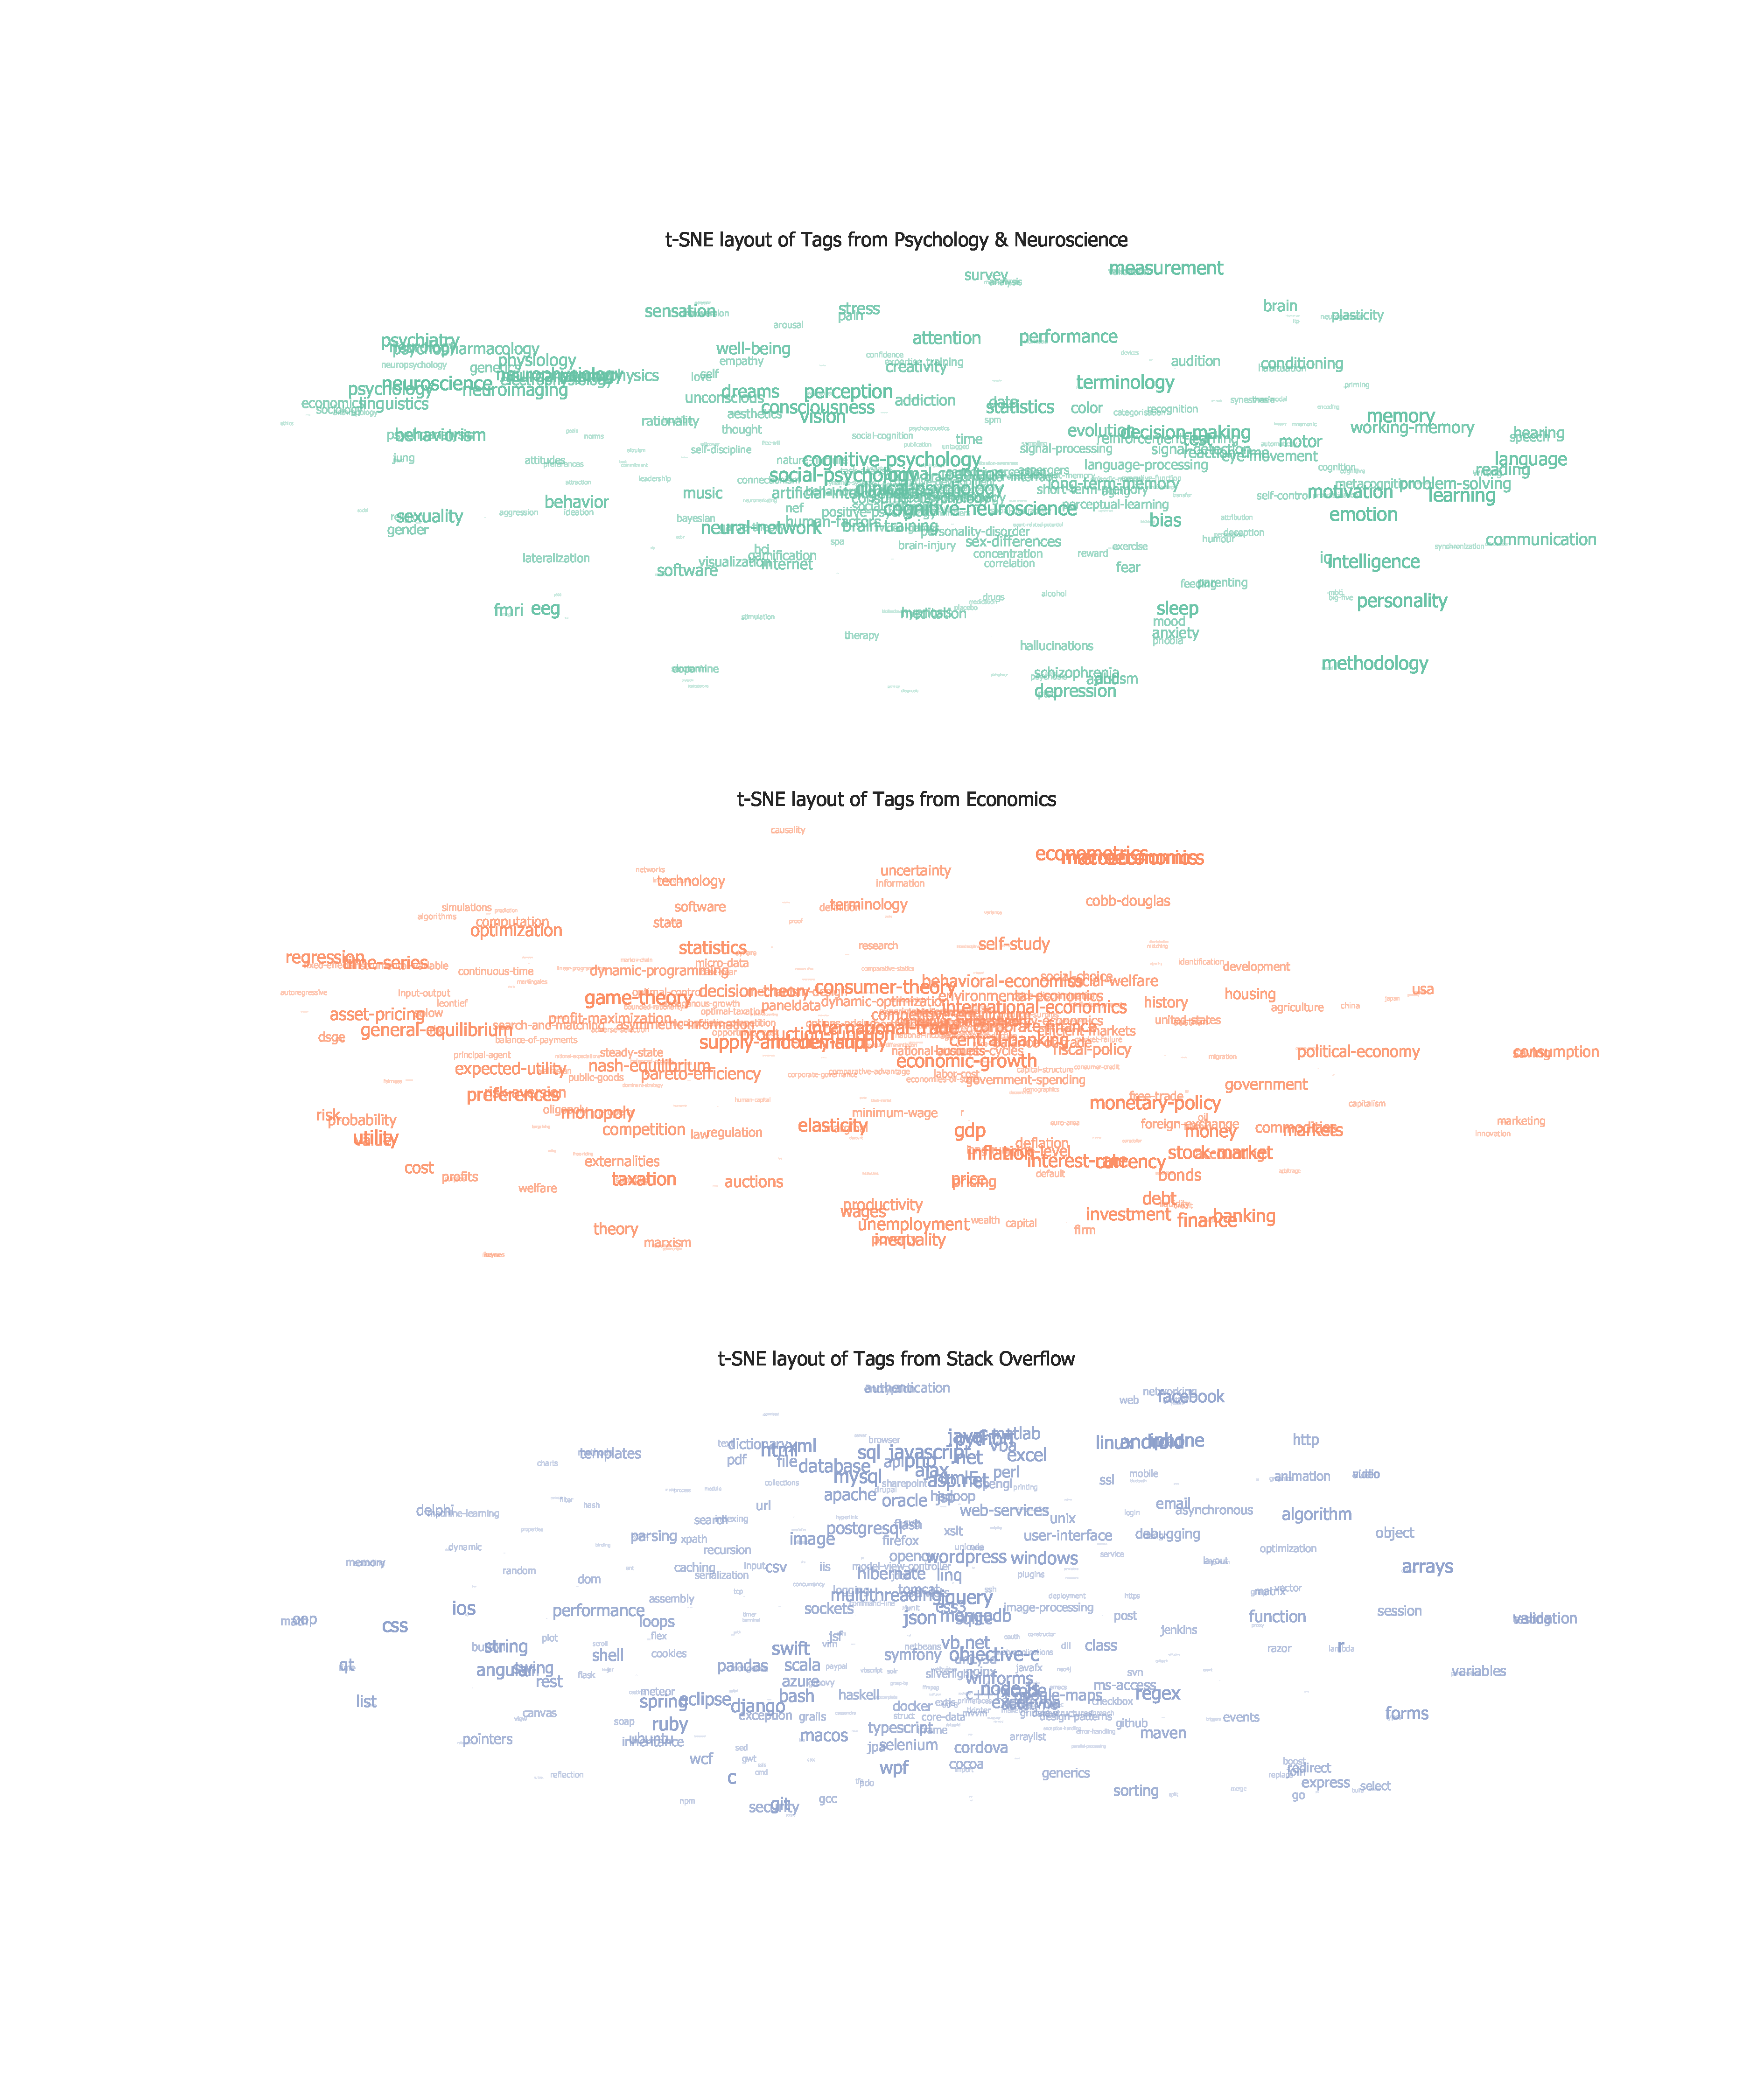
\includegraphics[height=1.1\textheight]{tsne_indv}
	\end{adjustbox}
	\caption{t-SNE reduction of tags from Stack Overflow, Economics and Psychology \& Neuroscience, sized by number of usages on the site}\label{tsne_indv}
\end{figure}

\begin{table}[ht]
	\centering
	\begin{adjustbox}{center}
		\begin{tabular}{lrrr}
			\toprule
			Site &  Total Tags &   Used Tags & Top Tags\\
			\midrule
			Stack Overflow &51671&374& \texttt{javascript},\texttt{java},\texttt{php}\\
			Economics &372&275&\texttt{macroeconomics}, \texttt{microeconomics},\texttt{econometrics}\\
			Psychology \& Neuroscience&348&296& \pbox{20cm}{\RaggedLeft\texttt{cognitive-psychology}, \texttt{social-psychology},\\ \texttt{neuroscience}}\\
			\bottomrule
		\end{tabular}
	\end{adjustbox}
	\caption{Stack exchange sites tag usage}\label{tags}
\end{table}

\begin{figure}[H]
	\centering
	\begin{adjustbox}{center}
		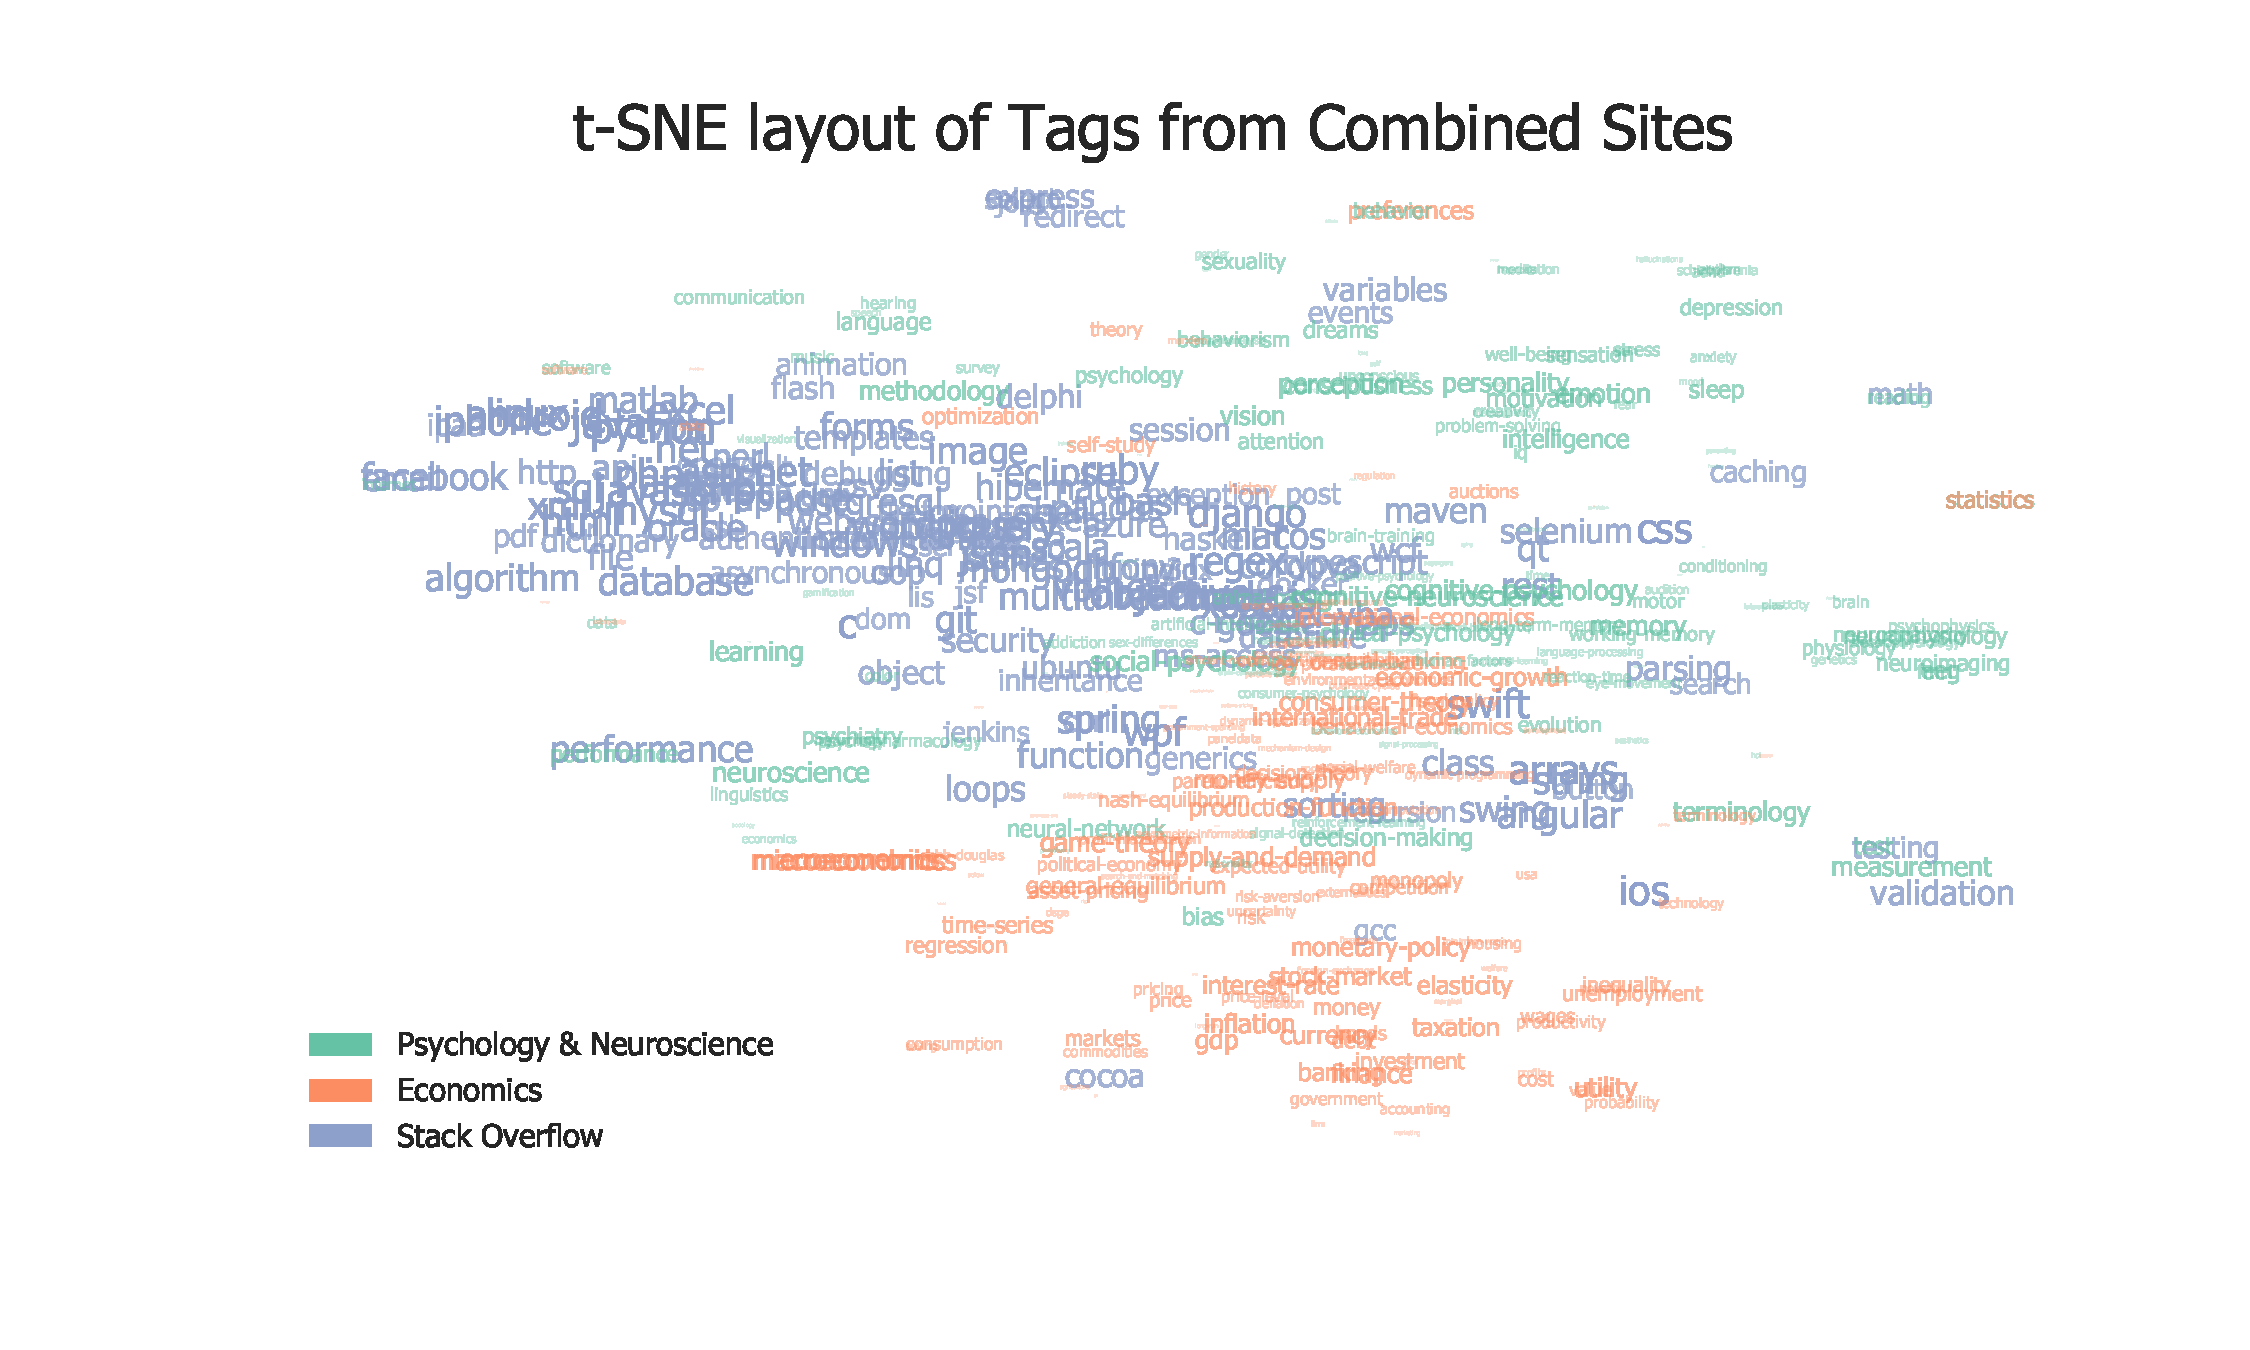
\includegraphics[height=.5\textheight]{tsne_combined}
	\end{adjustbox}
	\caption{t-SNE reduction of tags from Stack Overflow, Economics and Psychology \& Neuroscience combined, sized by number of usages on the site, notice some tags occur on multiple sites e.g. statistics}\label{tsne_combined}
\end{figure}

\begin{table}[h]
	\centering
	\begin{adjustbox}{center}
		\begin{tabular}{lllllll}
			\toprule
			{} &           C &      Python &       Sociology &           Statistic &   Computational &            Network \\
			\midrule
			&    \num{358}\num{-379} &         c++ &    anthropology &  kolmogorov-smirnov &      computation &           networks \\
			&  \num{46}:420423 &        perl &     criminology &         chi-squared &        numerical &      network-based \\
			& \num{46}:849\num{-854} &      prolog &       geography &    likelihood-ratio &       simulation &             system \\
			&    \num{267}\num{-276} &        java &      philosophy &                wald &      algorithmic &     networks-based \\
			& \num{53}:566\num{-574} &       c/c++ &    sociological &          chi-square &              cpu &         networking \\
			&    \num{545}\num{-565} &        ampl &      psychology &          two-sample &     mathematical &                hub \\
			& \num{53}:387\num{-391} &  javascript &    epistemology &           bootstrap &  computationally &  experiment-tation \\
			&  :1220\num{-1223} &      opengl &         marxist &           t-student &          runtime &               node \\
			&     xxx-xxx &      matlab &       economics &       durbin-watson &  parallelization &           topology \\
			&    \num{400}\num{-416} &     fortran &  historiography &              f-test &      scalability &              graph \\
			\bottomrule
		\end{tabular}
	\end{adjustbox}
	\caption{Selected words and their 10 nearested neighbours}\label{nearests}
\end{table}

\subsection{Comparison}

After training, the models from epoch 30 for each of the subject was selected and ran on all publications in each subject. The resulting percentage of predicted computational publications as compared to the number of explicitly computational publications is given in Table \ref{ret_sub}. We can see that for all but one subject, Other Social Sciences, there are predicted to be more computational publications than those just published in computational sources. To verify that the predictions are correct, samples were collected, both randomly and by selecting those at extrema. A properly done verification would require multiple coders separately coding hundreds of publications, but in my small sample, the results of the analysis appear to be satisfactory. Figure \ref{sample_comp} has an example of predicted computational paper from outside the explicitly computational sources, while Figure \ref{sample_not_comp} shows an example of a non-computational paper that the model thinks has signs of being computational. Comparing the two, it is evident that the neural network is not just looking for keywords, since the `PORTAL-LIBRARIES AND THE ACADEMY' paper has many `computational' words (see section \ref{word_count} for discussion).

There is also a another model to compare to. The complete model can also produce a table, Table \ref{ret_full}. The table for the complete model disagrees with the partial models somewhat in most cases, but in \textit{Media and Communication} the difference is significant. The extent to which the disagreement is significant can be explored more thoroughly by application of Cohen's $\kappa$ \citep{cohen1960coefficient}. Table \ref{kappas} gives the $\kappa$ values for each subject, the results are more pessimist than the confusion matrices imply, at $0.70$ as the highest value and $0.31$ the lowest. Applying Landis and Koch's well known heuristic \citep{landis1977measurement} we can classify the agreements as fair ($0.31$) to substantial ($0.70$ ). Additionally, because Cohen's $\kappa$ attempts to down weight based on possible random guessing, and as both models are heavily biased towards negative, the formula is penalizing the agreement. Thus while not perfect the models can be considerer to have fair agreement, supporting that they are indeed classifying based on the same underlying distribution.

Another way to compare the models is by sampling and comparing manually. Figures \ref{subTrue} and \ref{subFalse} show two papers where the models disagree.

\begin{table}[H]
	\centering
	\begin{adjustbox}{center}
		\begin{tabular}{lrrr}
			\toprule
			{} &  \pbox{20cm}{Percentage\\Explicitly Computational} &  \pbox{20cm}{Percentage\\Predicted Computational} &  Difference \\
			\midrule
			Psychology              &          \num{1.5} &          \num{7.9} &  \num{6.4} \\
			Educational Sciences    &         \num{10.7} &         \num{27.5} & \num{16.8} \\
			Sociology               &          \num{2.9} &          \num{7.1} &  \num{4.2} \\
			Political Science       &          \num{1.9} &         \num{12.4} & \num{10.5} \\
			Other Social Sciences   &          \num{3.4} &         \num{19.5} & \num{16.1} \\
			Media and Communication &         \num{39.0} &         \num{36.1} &  \num{-2.9} \\
			Law                     &          \num{0.8} &          \num{5.7} &  \num{4.9} \\
			Economics and Business  &         \num{13.2} &         \num{36.8} & \num{23.6} \\
			\bottomrule
		\end{tabular}
	\end{adjustbox}
	\caption{Comparison ratios of  explicitly computational publications and those predicted to be computational by individual models}\label{ret_sub}
\end{table}

\begin{table}[H]
	\centering
	\begin{adjustbox}{center}
		\begin{tabular}{lrrr}
			\toprule
			{} &   \pbox{20cm}{Percentage\\Explicitly Computational}  &  \pbox{20cm}{Percentage\\Predicted Computational} &  Difference \\
			\midrule
			Psychology              &  \num{1.464321} &  \num{7.052985} &   \num{5.588663} \\
			Educational sciences    & \num{10.685390} & \num{33.249575} &  \num{22.564185} \\
			Sociology               &  \num{2.903707} & \num{11.067687} &   \num{8.163981} \\
			Political science       &  \num{1.892202} & \num{12.397832} &  \num{10.505630} \\
			Other social sciences   &  \num{3.383526} & \num{19.429262} &  \num{16.045736} \\
			Media and communication & \num{38.975246} & \num{62.596464} &  \num{23.621218} \\
			Law                     &  \num{0.766612} &  \num{3.546499} &   \num{2.779887} \\
			Economics and business  & \num{13.173174} & \num{38.588952} &  \num{25.415778} \\
			\bottomrule
		\end{tabular}
	\end{adjustbox}
	\caption{Comparison ratios of  explicitly computational publications and those predicted to be computational by the full model, note that counts are slightly different due to differences }\label{ret_full}
\end{table}

\begin{figure}[H]
	\centering
	\begin{adjustbox}{center}
		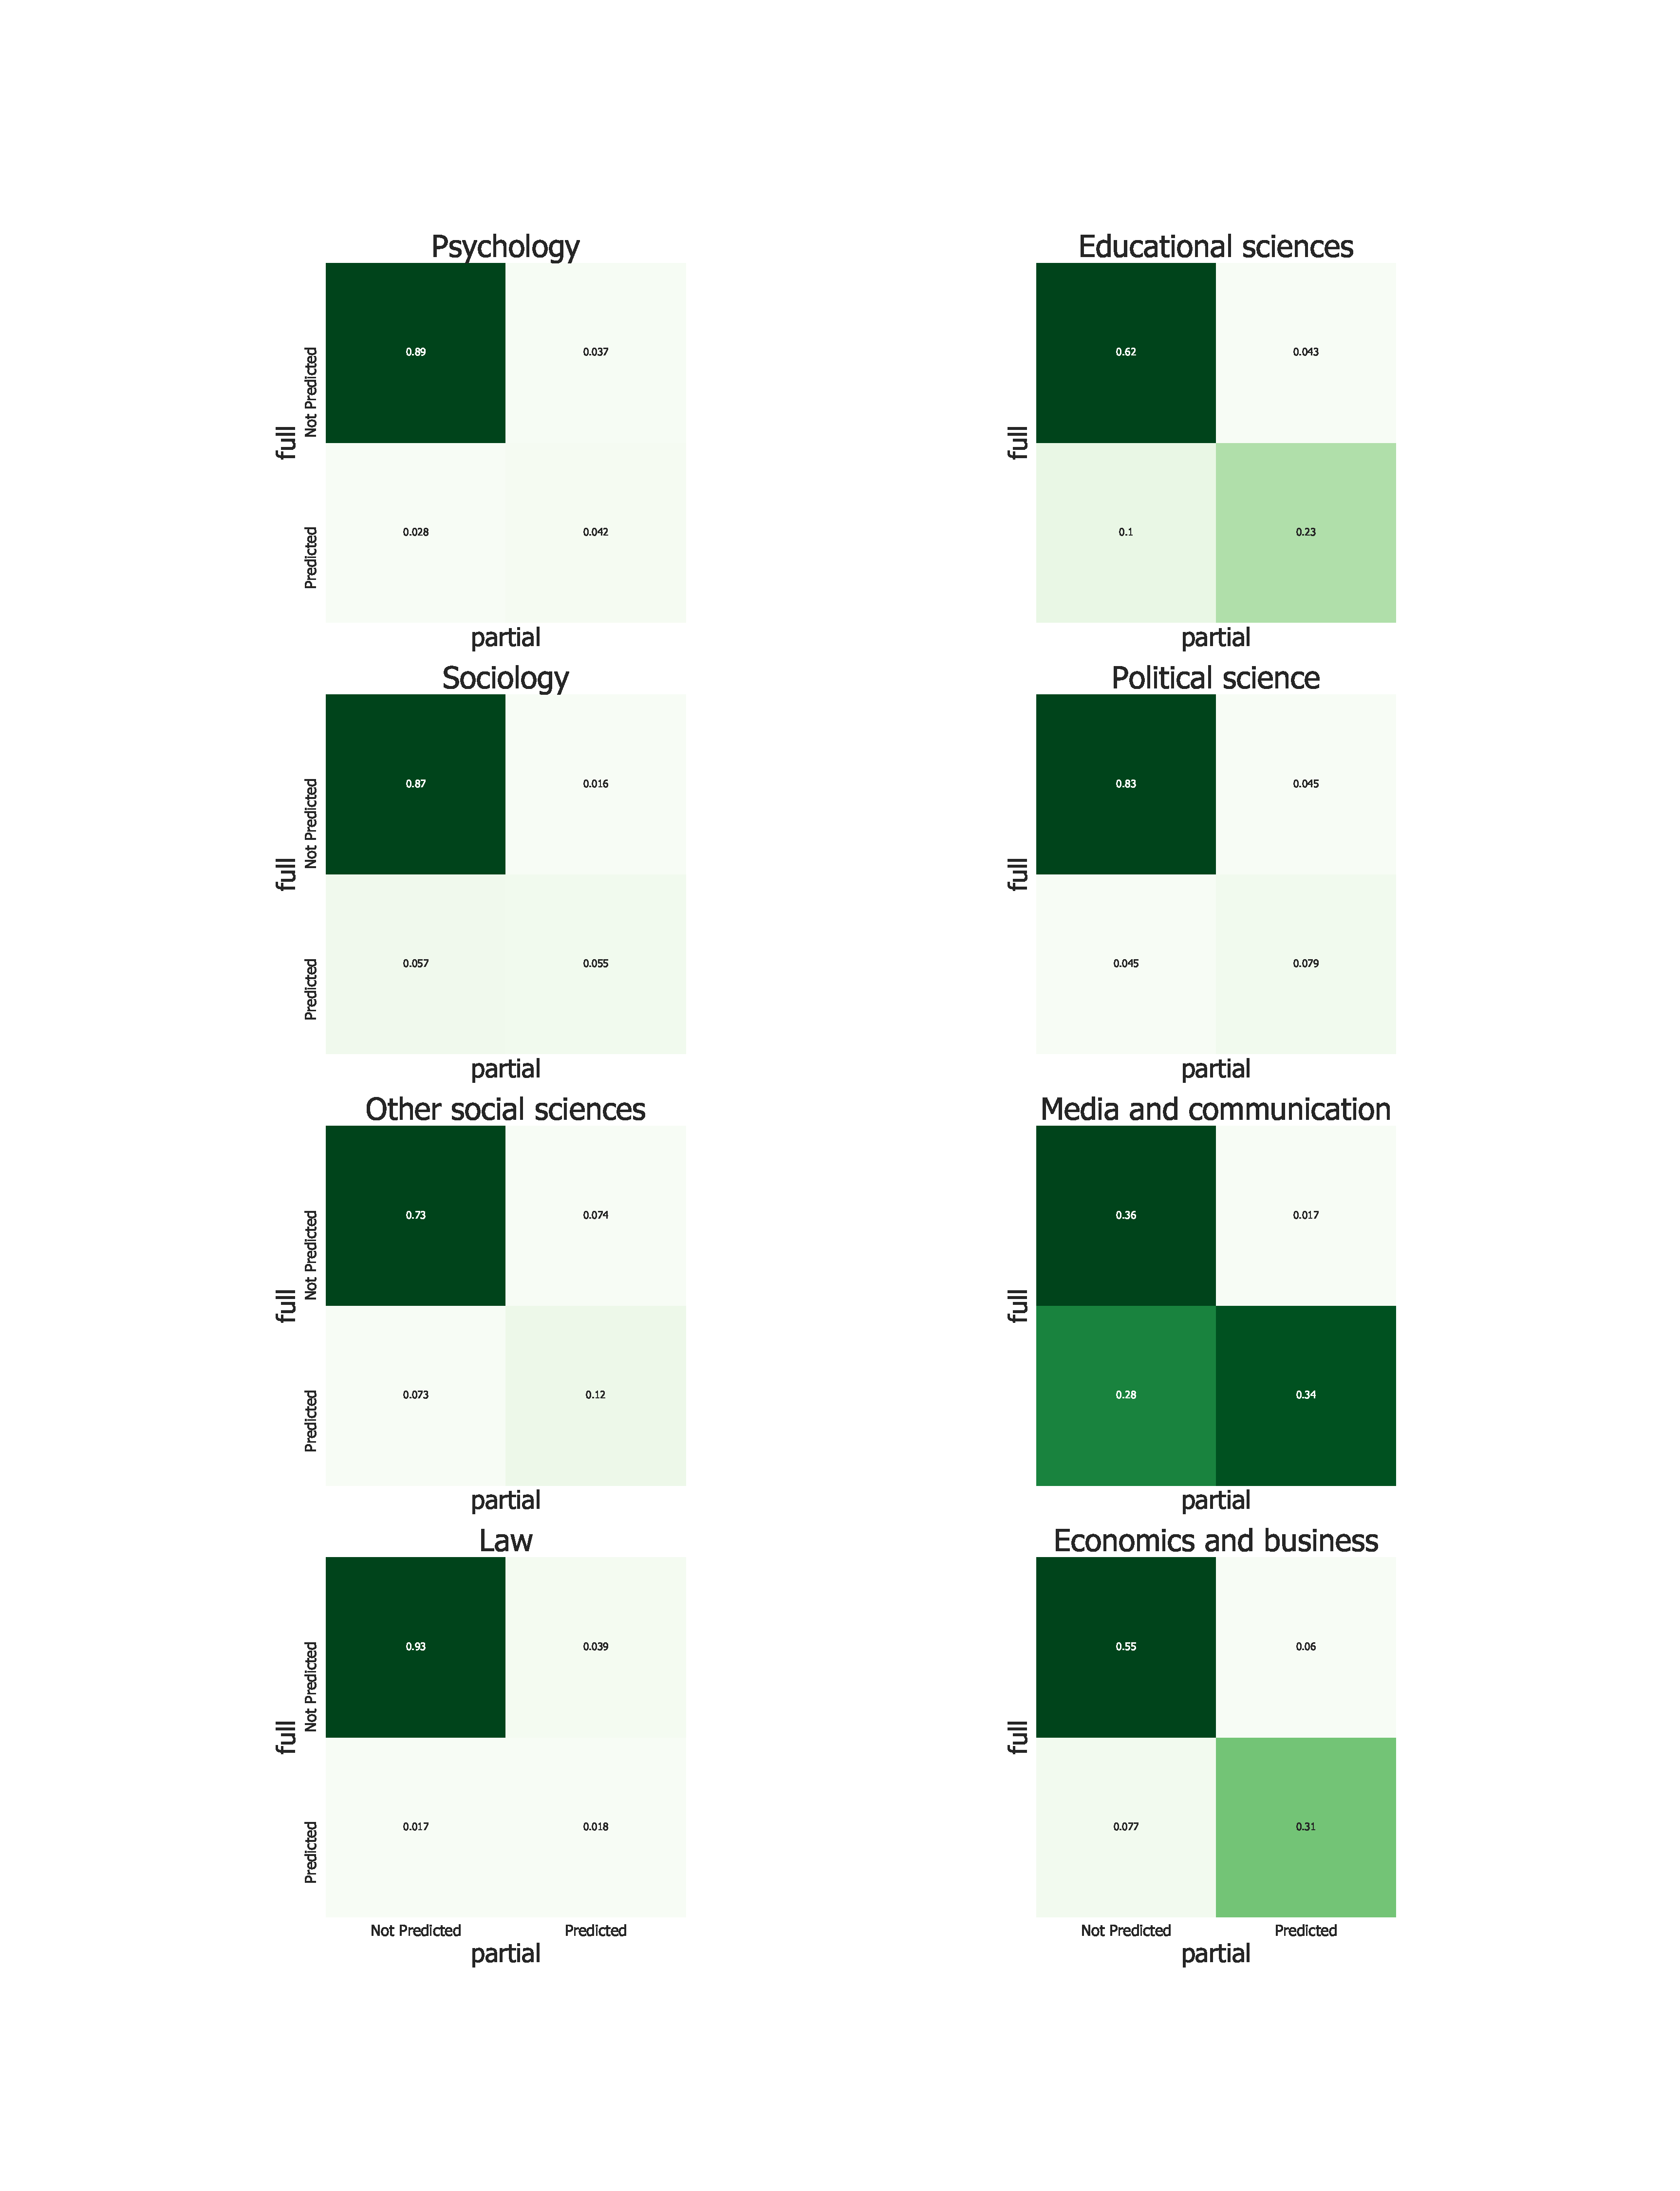
\includegraphics[width=\textwidth]{full_vs_partial}
	\end{adjustbox}
	\caption{Confusion matrices of full and subject based classifiers showing the normalized concurrence counts}\label{full_vs_partial}
\end{figure}

\begin{table}[H]
	\centering
	\begin{adjustbox}{center}
	\begin{tabular}{cccccccc}
		\toprule
		Psychology & \pbox{20cm}{Educational\\sciences} & Sociology & \pbox{20cm}{Political\\science} & \pbox{20cm}{Other social\\sciences} & \pbox{20cm}{Media and\\communication} & Law & \pbox{20cm}{Economics and\\business}\\
		\midrule
		\num{0.5028116216562004} & \num{0.616736670156338} & \num{0.366795474909127} & \num{0.3062451489371284} & \num{0.38751253484763193} & \num{0.46513269722412487} & \num{0.3142444446243683} & \num{0.7045478875428381}\\
		\bottomrule
	\end{tabular}
\end{adjustbox}
\caption{Cohen's $\kappa$ comparing the full and subject based classifiers}\label{kappas}
\end{table}

\begin{figure}[H]
	\begin{tabular}{ll}
		\toprule
		Field & Value\\
		\midrule
		ID & WOS:000206800000005 \\
		Explicitly Computational & False \\
		Likelyhood is Comp. Full& 45.1\% \\
		Likelyhood is Comp. Subject& 81.98\% \\
		Source &  JASSS-THE JOURNAL OF ARTIFICIAL\\
		& SOCIETIES AND SOCIAL SIMULATION \\
		Year of Publications & 2007.0 \\
		Title &  Higher-Order Simulations: Strategic Investment Under\\
		&Model-Induced Price Patterns \\
		\midrule
		Abstract &  The trading and investment decision processes in financial\\
		&markets become ever more dependent on the use of valuation\\
		&and risk models. In the case of risk management for\\
		&instance, modelling practice has become quite homogeneous\\
		&and the question arises as to the effect this has on the\\
		&price formation process. Furthermore, sophisticated\\
	\end{tabular}
\caption{Example of disagreement between subject and full models}\label{subTrue}
\end{figure}

\begin{figure}[H]
	\begin{tabular}{ll}
		\toprule
		Field & Value\\
		\midrule
		ID & WOS:000207690200005 \\
		Explicitly Computational & False \\
		Likelyhood is Comp.  Full& 60.4\% \\
		Likelyhood is Comp. Subject& 12.28\%\\
		Source & INTERNATIONAL JOURNAL OF HERITAGE STUDIES \\
		Year of Publications & 2008 \\
		Title &  Place as Dialogue: Understanding and Supporting the Museum\\
		&Experience \\
		\midrule
		Abstract &  This paper presents a dialogical approach to place, people\\
		&and technology in museums. The approach has been developed\\
		&in response to concern for locative experience in\\
		&Interaction Design, an approach to the design and\\
		&experience of interactive technologies that emphasises the\\
		&pivotal role played by a wide variety of relationships\\
		&in experience and suggests a set of dimensions of\\
		&experience that have been useful in our interpretations of \dots\\
		\bottomrule
	\end{tabular}
	\caption{Example of disagreement between subject and full models}\label{subFalse}
\end{figure}


\subsection{Introspection}

Another way to examine if the neural network is working the way it is expected to is to examine the output from the RNN section at each word. This is the layers $g^2$ and $h^2$ when they are combined. Since the last layer is a shallow one, we know it is working by taking the weighted sum of their outputs so that changes in the outputs lead to similar changes in the final output. Thus, while we cannot say that the value at index 85 is a significant factor, we can say that a change in many indices is correlated with indicates a change in the output. Figure \ref{visualize} shows the outputs as the RNN layers read the titles of each of the examples, and a comparison of their final results. By visual inspection, we can see that the word `based' in the positive example had a major impact while the colon in the negative started a major change in the negative example. This suggested that the model has identified `based on' as an indicator of computational papers, which is a valid suggestion. While the model has also identified that `: how` is an indicator of a negative example. Unfortunately, doing this type of analysis does not have a rigours backing from the literature, though some work is ongoing \citep{strobelt2018lstmvis}. As this type of deep introspection is quite new, there will hopefully be better tools developed within the next few years. So while this type of visuals can be useful, it cannot currently be the basis of decision making, and it is just a tool for inspecting the model.

\begin{figure}[ht]
	\begin{tabular}{ll}
		\toprule
		Field & Value\\
		\midrule
		ID & WOS:000318886700008 \\
		Explicitly Computational & False \\
		Likelyhood is Computational & 81.0\% \\
		Source &  APPLICATION AND BEST PRACTICE OF\\
		&COMPETITIVE TECHNICAL INTELLIGENCE \\
		Subject & Media and Communication\\
		Year of Publications & 2010 \\
		Title &  Research on the Key-technology Selection of Virtual\\
		&Reality Based on Patent Citation Analysis \\
		Citation & \cite{JianmeiWang}\\
		\midrule
		Abstract &  Based on the data of "Derwent Innovation Index" from 1963\\
		&to 2009, the authors construct a patent analysis dataset of\\
		&virtual reality by retrieving the patents through keywords\\
		&and classification numbers. The authors also reveal\\
		&technical hot points, key technologies of virtual reality\\
		&through patent citation analysis and multivariate\\
		&statistical analysis, and then acquire CTI (competitive\\
		&technical intelligence) for enterprises \dots \\
		\bottomrule
	\end{tabular}
\caption{Example of likely computational publication from a non-computational source}\label{sample_comp}
\end{figure}

\begin{figure}[ht]
	\begin{tabular}{ll}
		\toprule
		Field & Value\\
		\midrule
		ID & WOS:000306038900005 \\
		Explicitly Computational & False \\
		Likelyhood is Computational & 19.1\% \\
		Source & PORTAL-LIBRARIES AND THE ACADEMY \\
		Subject & Media and Communication\\
		Year of Publications & 2012 \\
		Title &  Incoming Graduate Students in the Social Sciences: How\\
		&Much Do They Really Know About Library Research? \\
		Citation & \cite{monroe2012incoming}\\
		\midrule
		Abstract &  Academic librarians provide information literacy\\
		&instruction and research services to graduate students. To\\
		&develop evidence-based library instruction and research\\
		&services for incoming graduate students, the authors\\
		&interviewed fifteen incoming graduate students in the\\
		&social sciences and analyzed the interviews using the\\
		&Association of College \& Research Libraries Information\\
		&Literacy Competency Standards for Higher Education (ACRL\\
		&Standards). This article discusses the findings, including\\
		&the authors' assumptions of student information illiteracy,\\
		&trends noted during the interview analysis, and\\
		&implications for delivering information literacy training\\
		&to graduate students in a group discussion modality. \\
		\bottomrule
	\end{tabular}
\caption{Example of possible non-computational publication from a non-computational source}\label{sample_not_comp}
\end{figure}

\begin{figure}[ht]
	\centering
		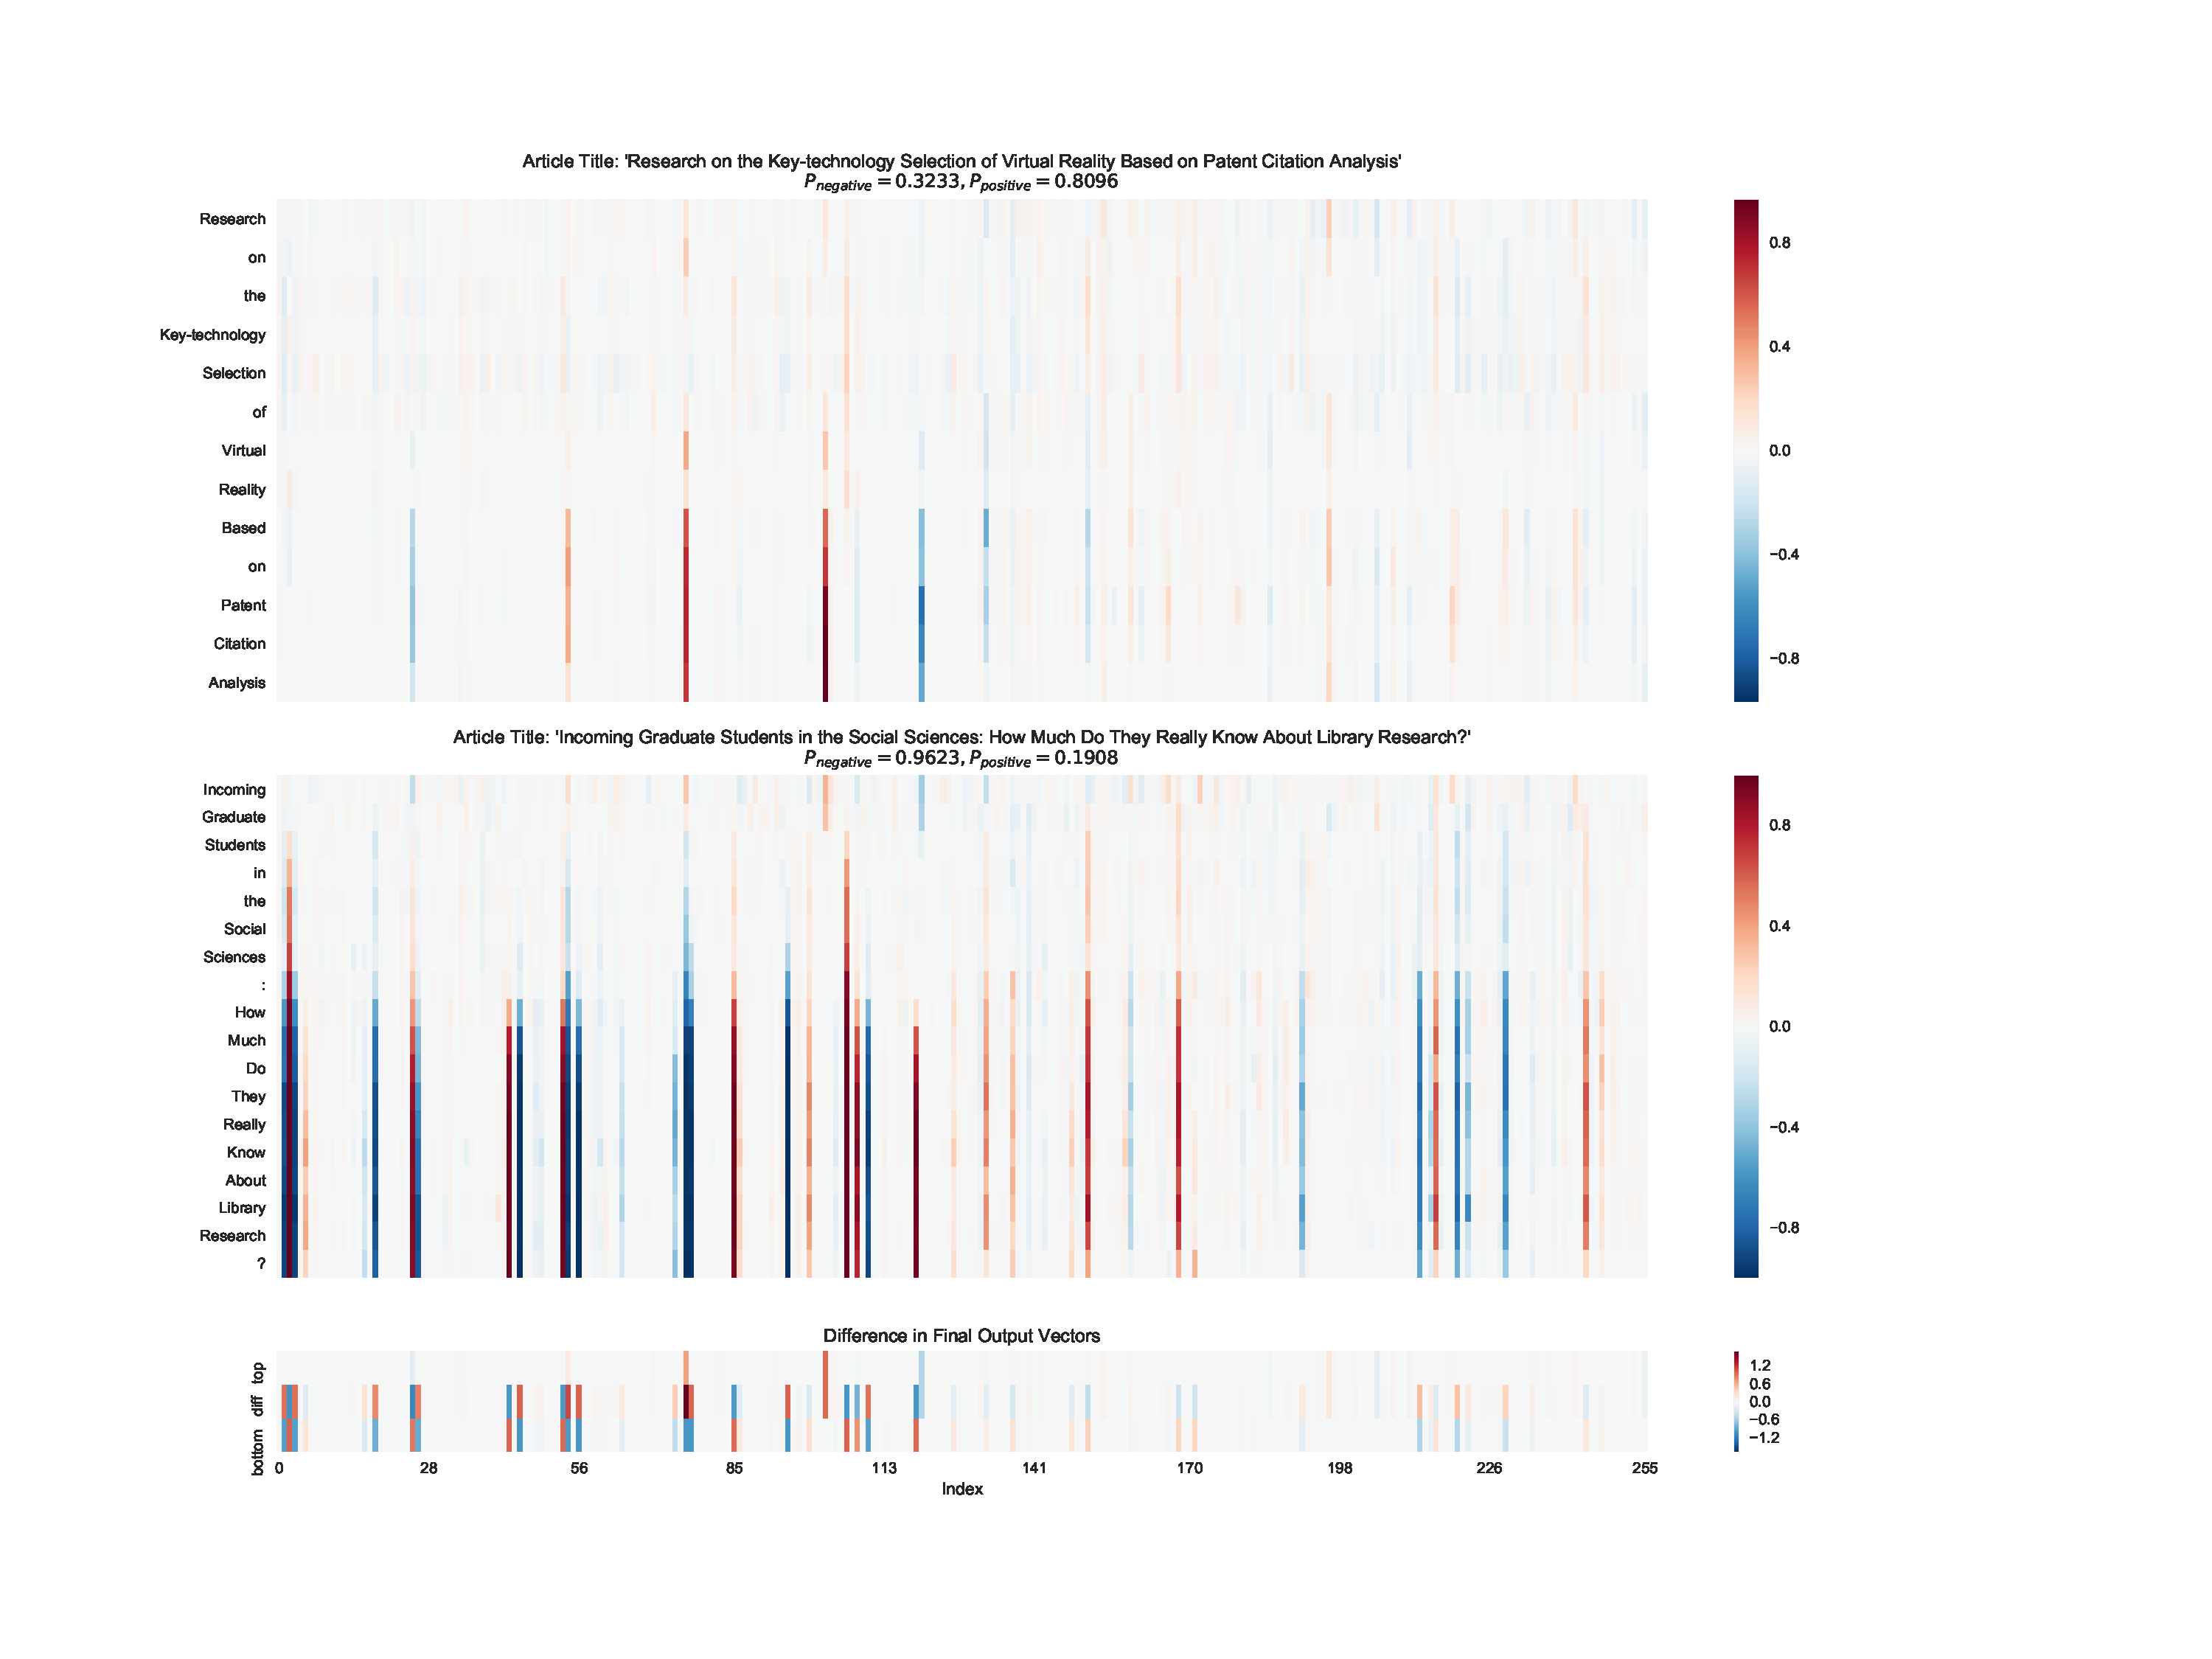
\includegraphics[width=\textwidth]{visualize}
	\caption{RNN activations for each word in two titles; the positive example is on top, the negative below it, and a comparison of each input's final output is shown at the bottom}\label{visualize}
\end{figure}

\subsection{Word Usage}\label{word_count}

Figure \ref{wc} shows a word cloud constructed from the titles of the computational and non-computational publications in Sociology. The word cloud is constructed by counting the number of occurrences of a word and sizing it according to the count, with the words then laid out algorithmically. This visualization lets us see what the relationship is between the words used in the two sets. We can see in particular that the computational publications refer to `based' much more than the non-computational ones, along with other words such as `Network', `System' and `Information', all of which are related to more analytical approaches. While the non-computational publications refer to`Relationship', `Social' and `Women' which suggest a more quantitative style of paper. Word clouds for each of the subjects can be found in Appendix \ref{appendix}.

\begin{figure}[H]
	\centering
	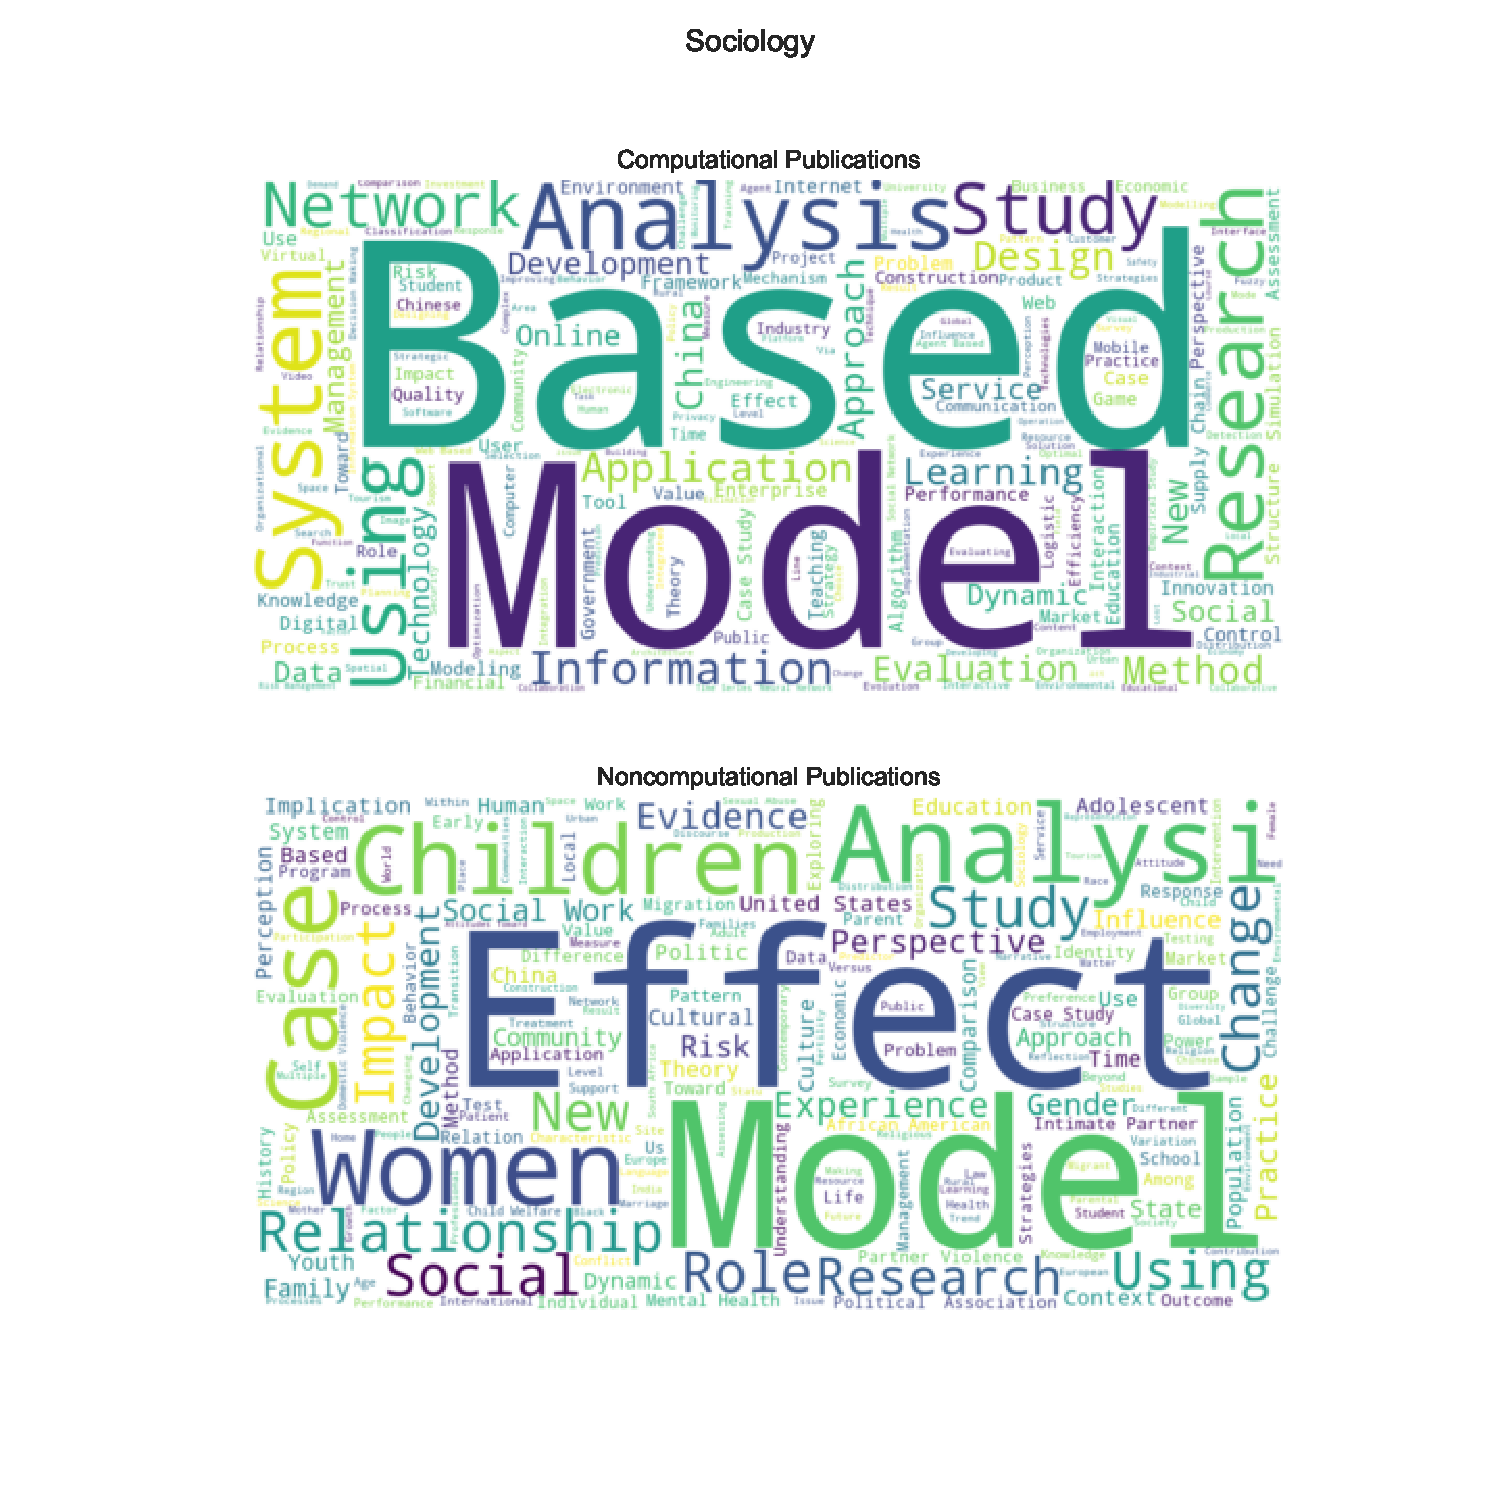
\includegraphics[width=\textwidth]{wc_Sociology}
	\caption{Word cloud of Sociology publication's titles}\label{wc}
\end{figure}

\subsection{Occlusion Effects}

A a method used to some success in convolutional neural network (CNN) visualization and introspection is the \textit{occlusion experiment}, where an image is broken into subsections and the CNN is asked to make a classification with the subsection removed \citep{zeiler2014visualizing}. This method allows one to measure the significance of each of the subsections by measuring how their removal affects the classification certainty. Figure \ref{oc1} shows the effects of removing words from the title and abstract on the classification probability for a toy example with the title of \textit{Exploration of humans, society and R} and abstract `\textit{We used methods and techniques to do stuff. Weber Freud and vocabulary acquisition were explored. Then we did more stuff. Our code can be found on Github.}'. We can see in the bottom left that if the title is \textit{Exploration} and the abstract simply \textit{We used methods and techniques to do stuff.} then the full model gives it a $0.64$ probability of being computational, but if you add the sentence \textit{Weber Freud and vocabulary acquisition were explored.} the probability drops to $0.41$. Similarly adding the final sentence \textit{Our code can be found on Github.} firmly puts the record as computational with a probability of $0.89$ and if \textit{R} is added to the title, the probability goes up to $0.95$.

This methodology adds support to the RNN classifying based in part on words, but also on word order. If the last sentence is put first in the abstract, the final model probability goes down by more than $20\%$. This method is explored much further on the interactive webapp hosted at \href{shiny.reidmcy.com/fp}{shiny.reidmcy.com/fp}. There is one major concern with making inferences with occlusion of this  type of model, which is that there is no baseline blank set of words. In image processing, the pixels can be coloured a uniform mixture with $50\%$ brightness (grey), while with word embeddings, there is no such null vector, thus removing the entire vector from the input is the best option. It would be simple to add a `removed' vector to the training, and that is an intriguing direction of future research.  

\begin{figure}[H]
	\centering
	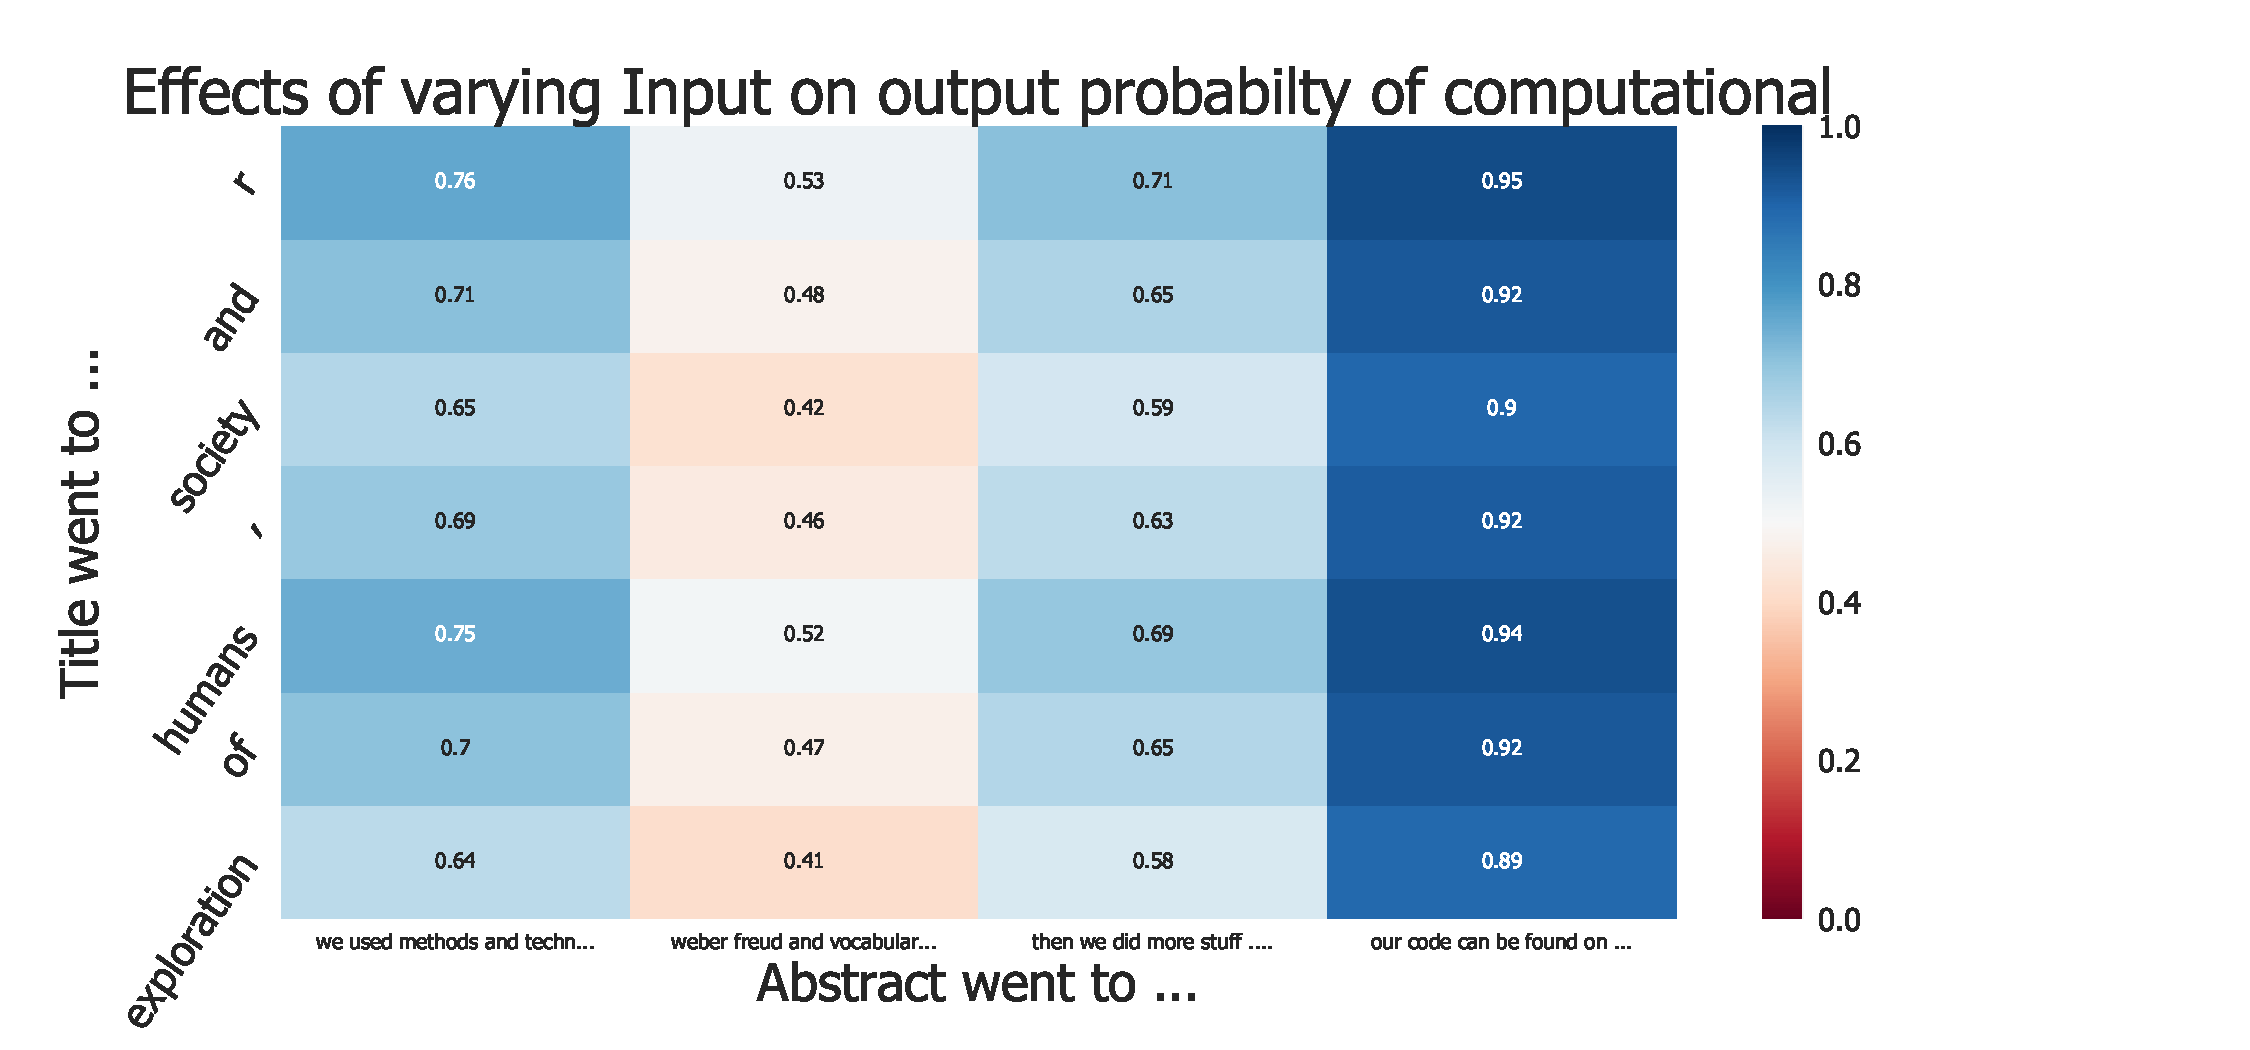
\includegraphics[width=1\textwidth]{occ}
	\caption{Model prediction as the title and abstract are added to, colour indicates the probability of the record being computational with blue being high and red low.}\label{oc1}
\end{figure}

\subsection{Temporal Effects}

Figure \ref{temporal} shows the number of computational papers per year for each of the subjects. The peak around 2007 for Media and Communications, and a couple others, is mostly due to some conferences (`International Conference on Information Management, Innovation Management and Industrial Engineering' contributes the most) being reclassified from Media and Communications to either a pure computer science or a more general subject (e.g. `Multidisciplinary Sciences') after 2008. What is notable is that the number of computational papers indicated by the model do follow the curve, but with a longer delay. Even as the conferences left the need to publish remained. Additionally, the low level of computational work is present in all disciplines. These are publications like `The application of virtual reality technology in interior design system development' \citep{chuanrong2016application}, which are discussions of computational techniques by members of the community for the community. In some cases they are like Boyle \citep{shapin1985leviathan}, attempting to layout a new programme of study to a sceptical audience who do not have the capabilities to observe the phenomena first-hand. While in others, the publications are completely integrated into the existing culture and communicating discoveries or designs of machines that are understood by the community \citep{cetina2009epistemic}. Distinguishing between the two classes of publications is a challenge that will likely be overcome at a later date, but for now I can only say that it seems that social scientists have not changed their discussion of computational  techniques by a significant amount in the last decade, baring some decreases in Psychology, Sociology and Economics.

\begin{figure}[H]
	\centering
	\begin{adjustbox}{center}
		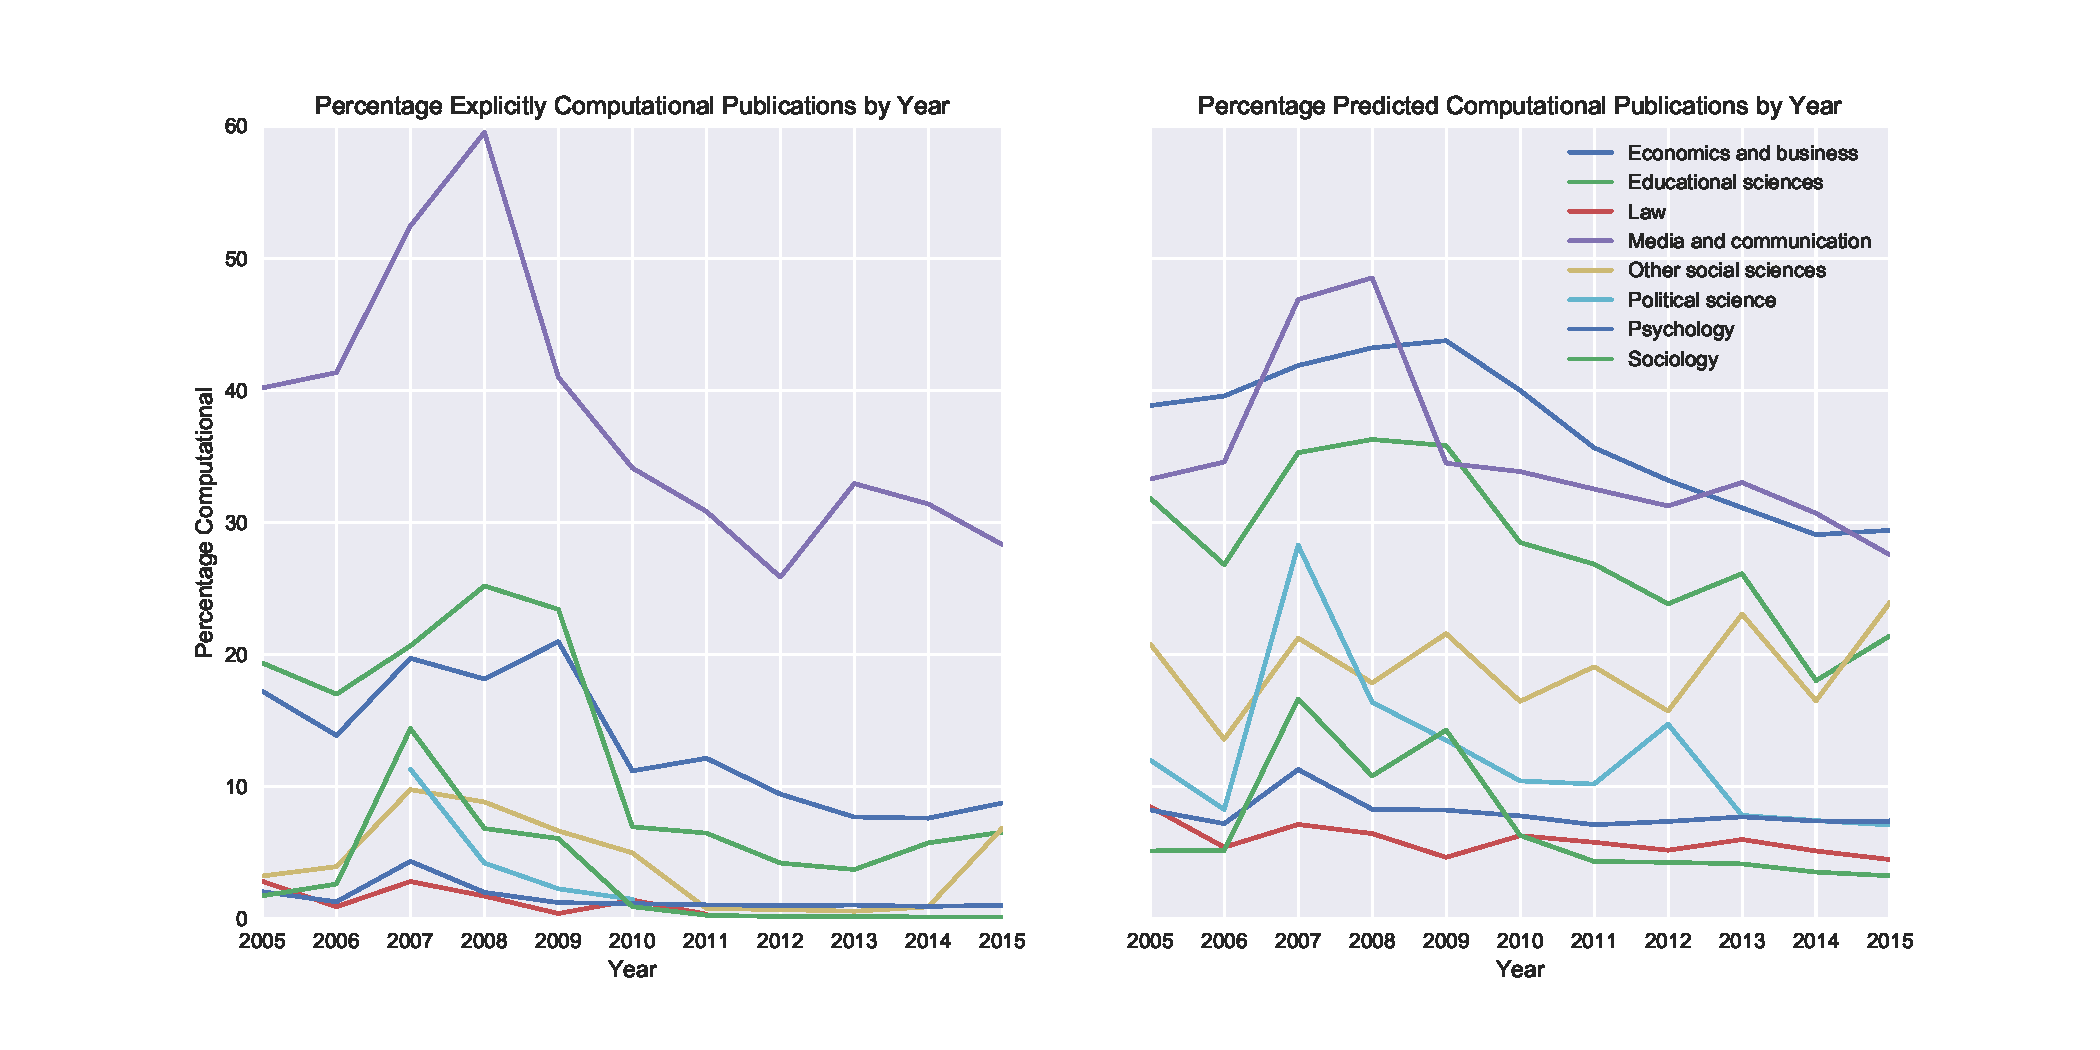
\includegraphics[width=1.2\textwidth]{temporal}
	\end{adjustbox}
	\caption{Yearly percentages of explicitly computational and predicted computational papers, notice the higher base line for the predicted papers and the smoother yearly transitions }\label{temporal}
\end{figure}

\subsection{Authors}

Figure \ref{auths} shows the smoothed probability density of the number of publications per author across computational and non-computational publications. The number of publications by each author was counted, then their counts were distributed from 0 to 20, with higher counts being cut down to 20 (thus the bump for a few subjects). Then a kernel density estimator with a bandwidth of .5 was used to interpolate and smooth, giving the continuous probability densities displayed.

The difference between the peaks of most computational and non-computational works is not surprising, as most psychologists aren't writing software. What is more surprising is the ones with overlap. High degrees of overlap suggests that  computational approaches are an excepted and normal means of doing science for that community. Maybe these computational people are forming their own community with it's own mediums of exchange with the outside world \citep{star1989institutional} or they are integrated into the knowledge society \citep{cetina2009epistemic}. More research on the subject would be required to answer this.

\begin{figure}[H]
	\centering
	\begin{adjustbox}{center}
		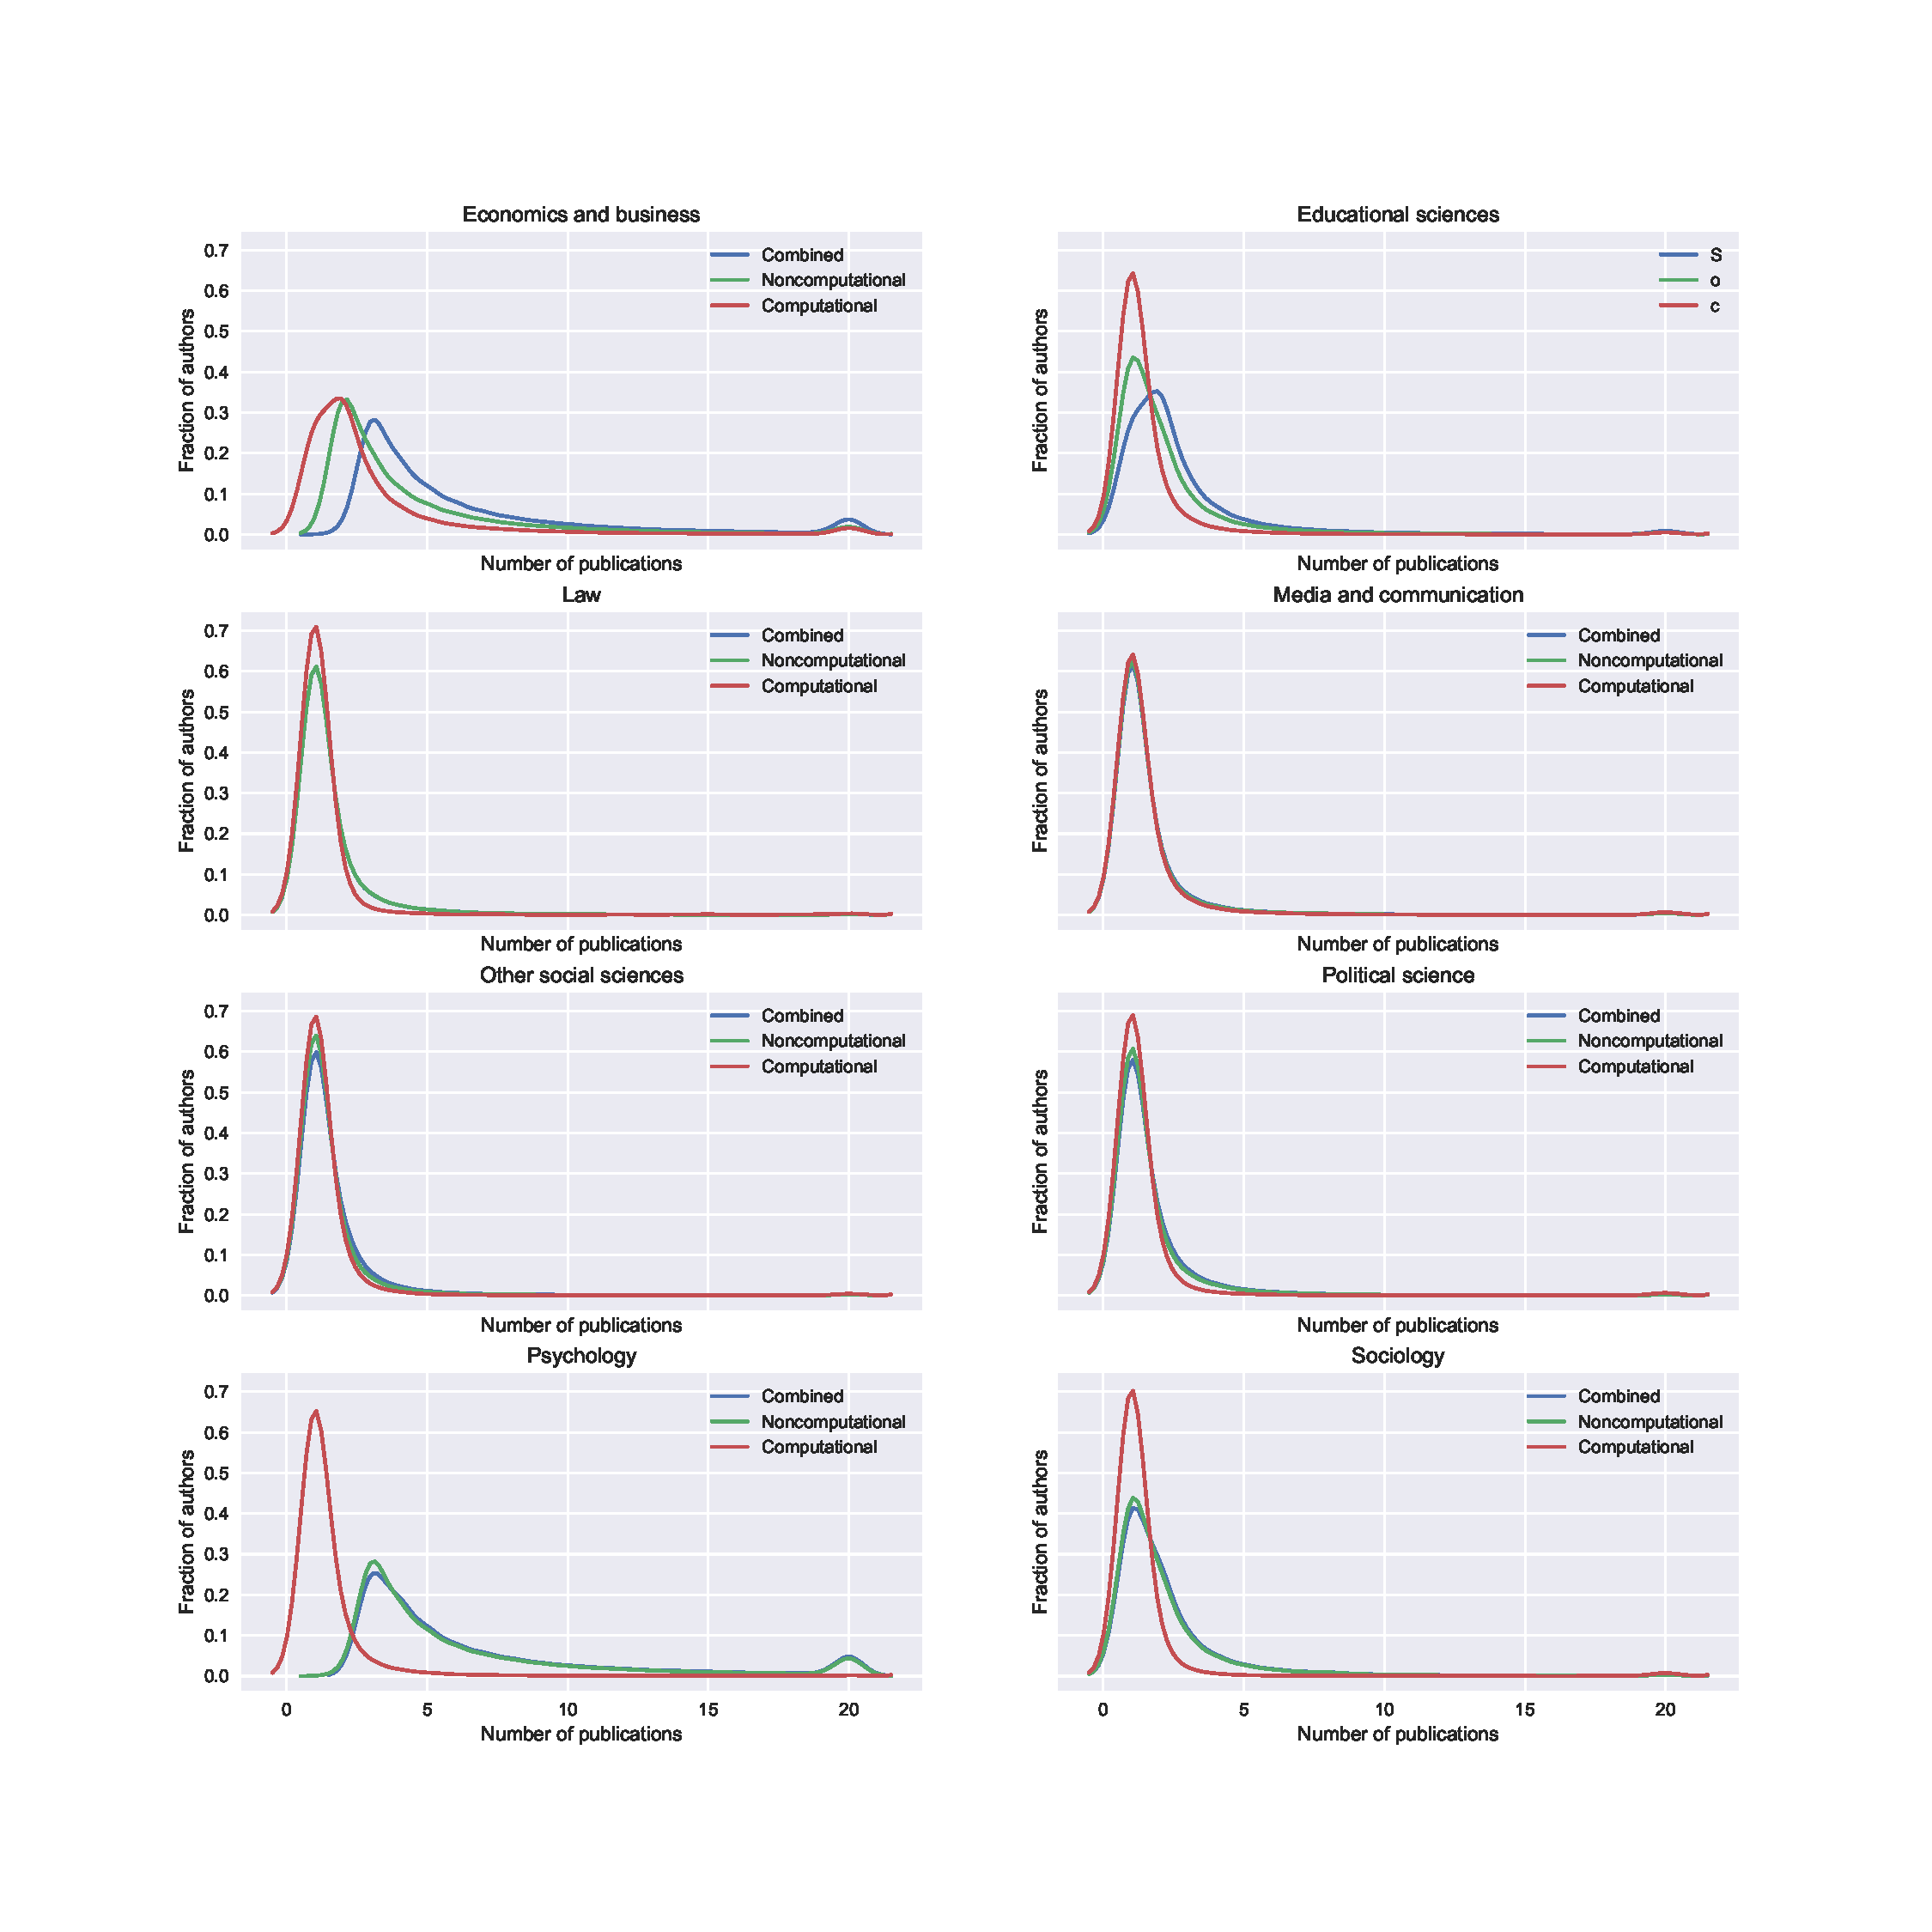
\includegraphics[width=1.2\textwidth]{auths_dist}
	\end{adjustbox}
	\caption{Probability density of the number of publication for a random author from either the computational, noncomputational or combined pool of publications in a subject}\label{auths}
\end{figure}


\section{Discussion}

\subsection{What is being classified}

Unlike the more traditional techniques discussed in Section \ref{ness}, deep neural networks' decision making processes are not well understood \citep{deep_learning_chapter12}. This limits understanding to inferences based on the observed outputs and inputs. The nominal goal of the classifier describe above is to identify computational usage across disciplines. But that is not what the training and testing data are measuring against. The data provided are collections of works from selected journals. What the journals impose on the papers, in particular upon their abstracts, that is different from the non-computational journals, is what the models are trained to identify. While there are certainly a much higher percentage of computational papers in the journals, as was shown above, they are not the sole holders of the computational keys. It is probably more accurate to characterize the classifications to being derived from the style of the abstract and title than the substance.

Then again, what makes a paper computational if not the style. Computer science existed well before computers could be produced, e.g. Leibniz's difference engine or Ada Lovelace's Note G. It could be considered that computational social science is as much a style of work as it is a set of methods. In \textit{Bit by Bit} Matthew Salganik \citep{salganik2017bit} describes many types of computational experiment, but the analysis required for some of them would not be unfamiliar to Kurt Lewin \citep{lewin1939field} as all that changes is that the data are collected without the experimenters leaving their lab. What make a research topic computational is the style of the approach, collection of all data possible and maybe more complex modelling at the end, not the substance. Thus looking for computational style might be the correct way to consider the problem of discovering computational usage.

\subsection{Results}

These results are not the definitive word on the distribution of computational methods across the social sciences, they are though a starting point. That this type of analysis produces anything at all except for noise shows that the deep neural network approach to complex, unstructured text is worth exploring and I plan to continue with it, hopefully improving accuracy and definitely better mapping out how long these tasks will take. 

In addition to the improvements, there are two problems with the current analysis that will need to be addressed. First, the usage of journals as the basis of the initial classification is very coarse, so either a better method needs to be created or more human coding must be done. Unfortunately, for the former method, a simple heuristic or machine learning approach can't be used as then the neural network would learn that instead of the correct distinction \citep{deep_learning_chapter12}. Thus, my preferred solution is to reduce the training time and train a series of networks, with the outputs from each generation being used to enrich the next one's training data. This has the downside of requiring a large amount of human intervention though. The other issue with this result is that it cannot be generalized. The usage of word embedding trained on the complete universe of interest means that if a new record is to be considered, the embedding has to be redone, or at least updated, which in either case requires a complete retraining of the model. Even with these two issues, there are some useful results, and both can be mediated with further work.

\subsection{Further Steps}

The baseline activity in computation across all subjects is very intriguing, as it suggests that computational approaches may not be as divisive as some suggest \citep{watts2007twenty}\citep{lazer2009life}. There is already precedent for scientists to accept and use new tools, machinery or ideas, without having to change their paradigm. The Latourian idea of a black box \citep{latour1987science} can be used to describe many computational techniques. Do everyday scientists care about how the line of the linear regression is derived? No, they only care about the fact that it is accurate, so why would it matter if a graduate student or a computer made it? The techniques may be more complicated than a linear regression, but that may require a new sex added to the seven sexes of Collins \citep{collins1975seven}, focused on complex computational systems to be needed for replication, but will it require a fundamental shift in methodology? 

An additional point of particular interest that this would form the basis of answering, is `how do new styles/methods diffuse through science?' There is much work already on the diffusion of knowledge \citep{griliches1960hybrid} \citep{crane1972invisible} \citep{evans2010industry}, but there is much less work on diffusion of style or technique. The data provided by this method combined with bibliographic analysis would likely reveal some interesting results. Additionally, the method is not limited to identifying computational approaches it can be trivially generalized given the correct training data. Of note, instead of binary classification, a mixture model could be created, where different styles exist in different proportions in each record thus along the competition of styles to be considered.

There are a few more aspects, particular to Science Studies, that were not able to be a part of this analysis. First, examining the impact of gender on computational publications. Women's representation in software development is low, but is it also low in scientific computation? Secondly, how do computational researchers fit into the modes of science already in place, e.g. can computational sociology coexist with the strong programme \citep{bloor1976strong}? This work suggests that they can fit in well. Finally, is the advent of computational social science a paradigm shift? Or is just another set of black box to help scientists to get slightly closer to the truth?

\newpage
\singlespacing
\setcounter{page}{1}
\pagenumbering{roman}
\addcontentsline{toc}{section}{References}
\bibliography{Report}{}

\bibliographystyle{asr}


\appendix
\section{Appendix: Complete table of WOS Social Science subject tags}\label{app_tags}
\begin{table}[H]
	\centering
	\rowcolors{2}{gray!25}{white}
	\begin{adjustbox}{center}
		\small
		\begin{tabular}{l|rr}
			\toprule
			\rowcolor{gray!50}
			Subject &WOS Code&Subsubject \\
			\midrule
			5.01 Psychology                    & BV & PSYCHOLOGY, BIOLOGICAL                    \\
			5.01 Psychology                    & CN & BEHAVIORAL SCIENCES                       \\
			5.01 Psychology                    & HI & PSYCHOLOGY, EDUCATIONAL                   \\
			5.01 Psychology                    & JI & ERGONOMICS                                \\
			5.01 Psychology                    & MY & PSYCHOLOGY, DEVELOPMENTAL                 \\
			5.01 Psychology                    & NQ & PSYCHOLOGY, APPLIED                       \\
			5.01 Psychology                    & VI & PSYCHOLOGY                                \\
			5.01 Psychology                    & VJ & PSYCHOLOGY, MULTIDISCIPLINARY             \\
			5.01 Psychology                    & VS & PSYCHOLOGY, MATHEMATICAL                  \\
			5.01 Psychology                    & VX & PSYCHOLOGY, EXPERIMENTAL                  \\
			5.01 Psychology                    & WQ & PSYCHOLOGY, SOCIAL                        \\
			5.02 Economics and business        & DI & BUSINESS                                  \\
			5.02 Economics and business        & DK & BUSINESS, FINANCE                         \\
			5.02 Economics and business        & GY & ECONOMICS                                 \\
			5.02 Economics and business        & NM & INDUSTRIAL RELATIONS \& LABOR             \\
			5.02 Economics and business        & PC & MANAGEMENT                                \\
			5.02 Economics and business        & PE & OPERATIONS RESEARCH \& MANAGEMENT SCIENCE \\
			5.03 Educational sciences          & HA & EDUCATION \& EDUCATIONAL RESEARCH         \\
			5.03 Educational sciences          & HB & EDUCATION, SCIENTIFIC DISCIPLINES         \\
			5.03 Educational sciences          & HE & EDUCATION, SPECIAL                        \\
			5.04 Sociology                     & BF & ANTHROPOLOGY                              \\
			5.04 Sociology                     & FU & DEMOGRAPHY                                \\
			5.04 Sociology                     & JM & ETHNIC STUDIES                            \\
			5.04 Sociology                     & JO & FAMILY STUDIES                            \\
			5.04 Sociology                     & PS & SOCIAL SCIENCES, MATHEMATICAL METHODS     \\
			5.04 Sociology                     & WM & SOCIAL ISSUES                             \\
			5.04 Sociology                     & WY & SOCIAL WORK                               \\
			5.04 Sociology                     & XA & SOCIOLOGY                                 \\
			5.04 Sociology                     & ZK & WOMEN'S STUDIES                           \\
			5.05 Law                           & FE & CRIMINOLOGY \& PENOLOGY                   \\
			5.05 Law                           & OM & LAW                                       \\
			5.06 Political science             & OE & INTERNATIONAL RELATIONS                   \\
			5.06 Political science             & UU & POLITICAL SCIENCE                         \\
			5.06 Political science             & VM & PUBLIC ADMINISTRATION                     \\
			5.07 Social and economic geography & BM & AREA STUDIES                              \\
			5.07 Social and economic geography & JB & ENVIRONMENTAL STUDIES                     \\
			5.07 Social and economic geography & KU & GEOGRAPHY                                 \\
			5.07 Social and economic geography & UQ & PLANNING \& DEVELOPMENT                   \\
			5.07 Social and economic geography & YQ & TRANSPORTATION                            \\
			5.07 Social and economic geography & YY & URBAN STUDIES                             \\
			5.08 Media and communication       & EU & COMMUNICATION                             \\
			5.08 Media and communication       & NU & INFORMATION SCIENCE \& LIBRARY SCIENCE    \\
			5.09 Other social sciences         & MW & HOSPITALITY, LEISURE, SPORT \& TOURISM    \\
			5.09 Other social sciences         & OR & ASIAN STUDIES                             \\
			5.09 Other social sciences         & EN & CULTURAL STUDIES                          \\
			5.09 Other social sciences         & WU & SOCIAL SCIENCES, INTERDISCIPLINARY    \\
			\bottomrule
		\end{tabular}
	\end{adjustbox}
	\caption{Complete table of WOS Social Science subject tags}\label{sum_1}
\end{table}

\section{Appendix: Word Clouds}\label{appendix}
\begin{figure}[H]
	\centering
	\includegraphics[width=\textwidth]{wc_Economics_And_Business}
	\caption{Word cloud of Economics And Business publication's titles}
\end{figure}
\begin{figure}[H]
	\centering
	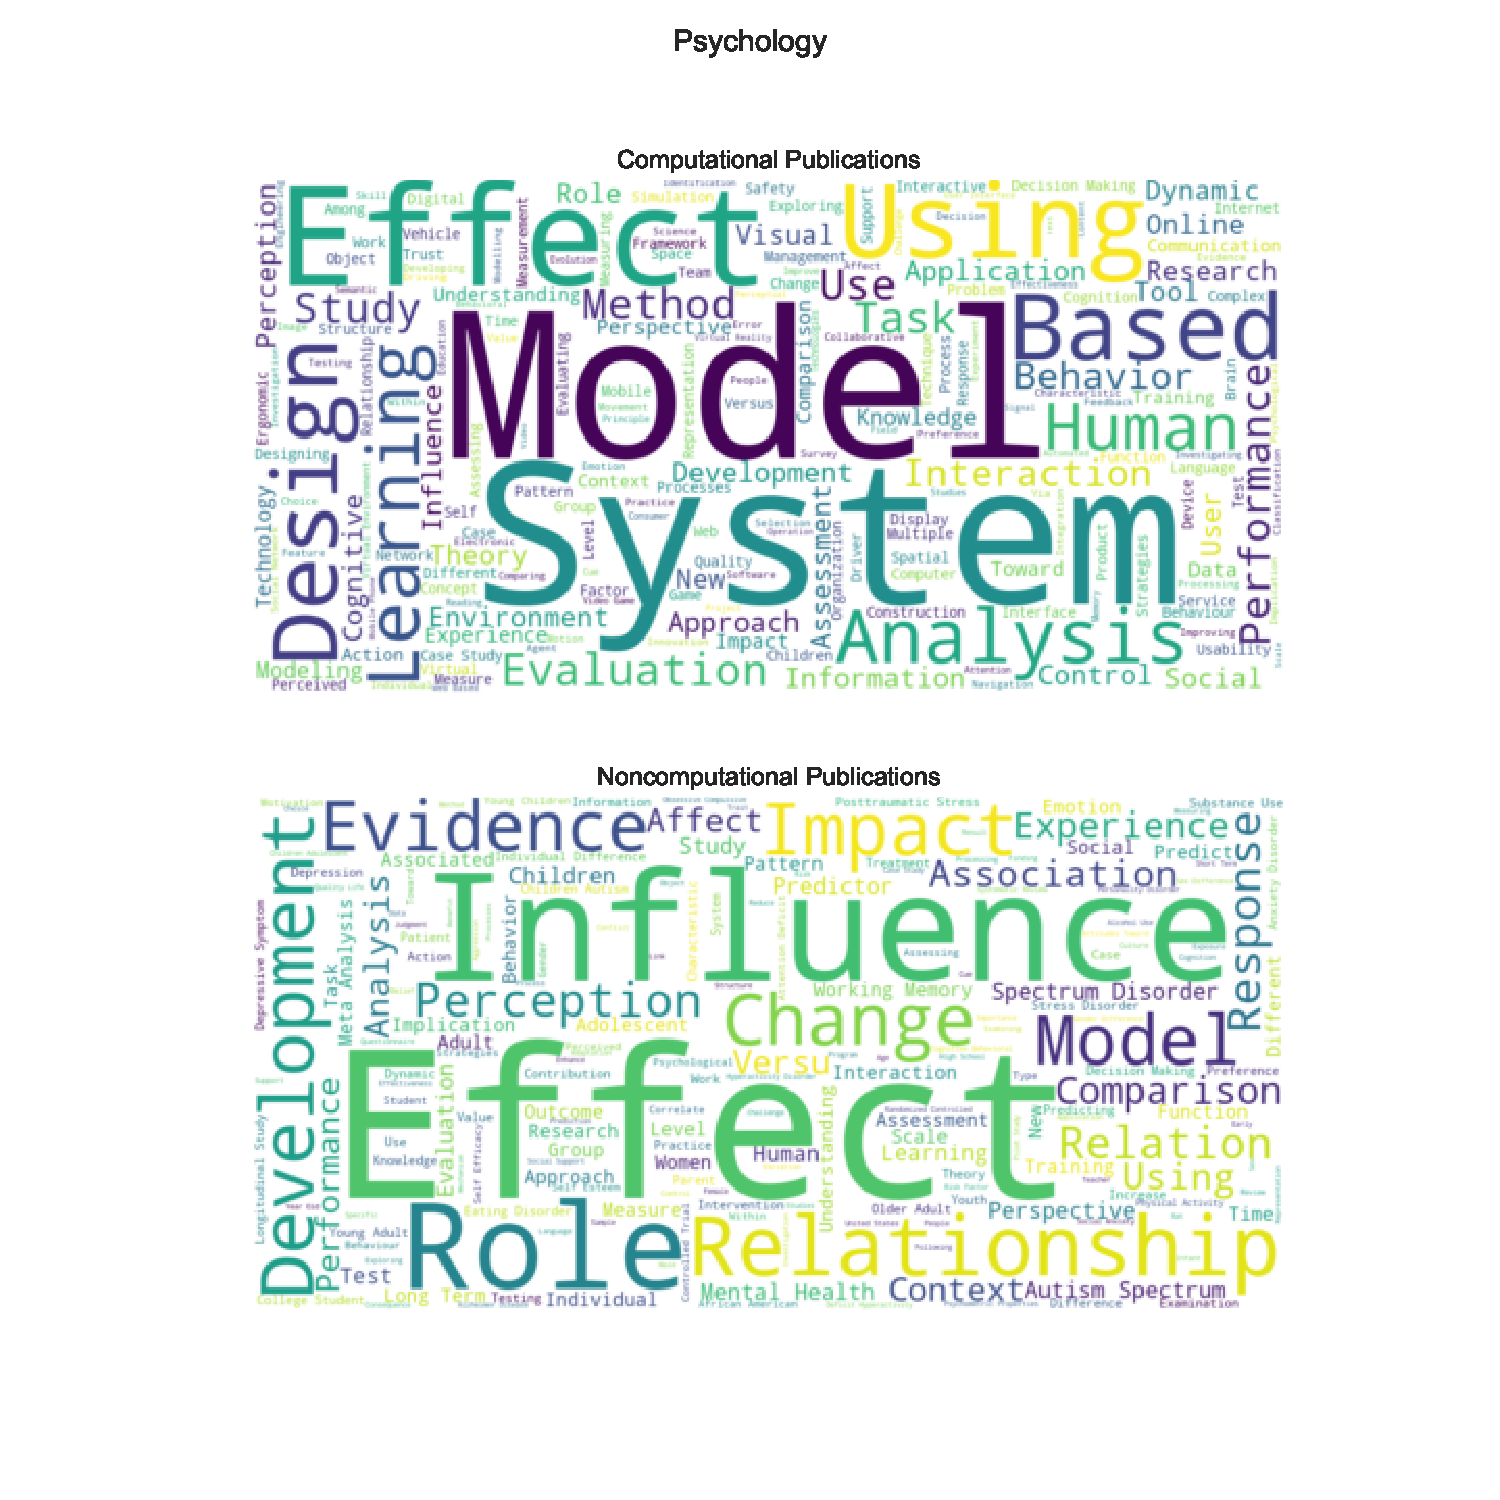
\includegraphics[width=\textwidth]{wc_Psychology}
	\caption{Word cloud of Psychology publication's titles}
\end{figure}
\begin{figure}[H]
	\centering
	\includegraphics[width=\textwidth]{wc_Educational_Sciences}
	\caption{Word cloud of Educational Sciences publication's titles}
\end{figure}
\begin{figure}[H]
	\centering
	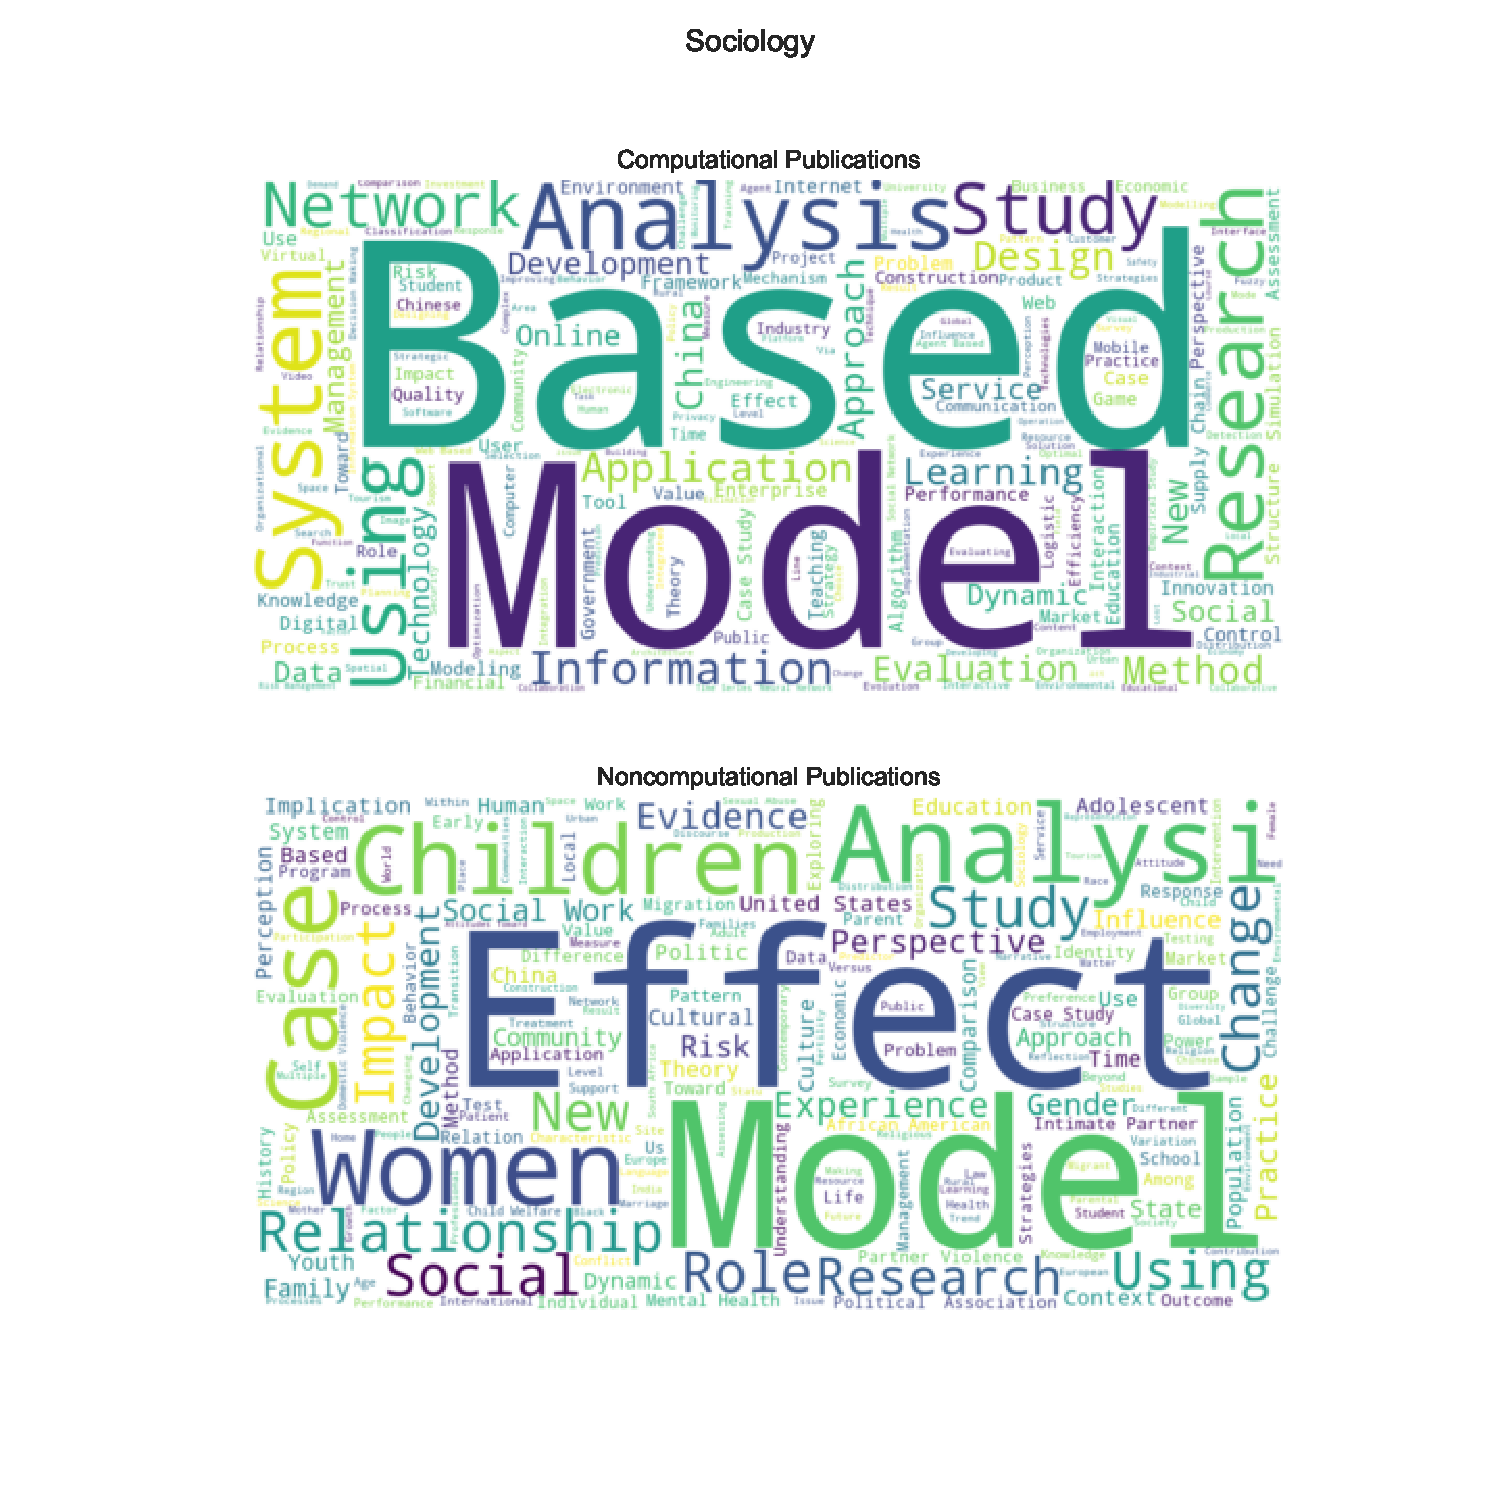
\includegraphics[width=\textwidth]{wc_Sociology}
	\caption{Word cloud of Sociology publication's titles}
\end{figure}
\begin{figure}[H]
	\centering
	\includegraphics[width=\textwidth]{wc_Political_Science}
	\caption{Word cloud of Political Science publication's titles}
\end{figure}
\begin{figure}[H]
	\centering
	\includegraphics[width=\textwidth]{wc_Other_Social_Sciences}
	\caption{Word cloud of Other Social Sciences publication's titles}
\end{figure}
\begin{figure}[H]
	\centering
	\includegraphics[width=\textwidth]{wc_Media_And_Communication}
	\caption{Word cloud of Media And Communication publication's titles}
\end{figure}
\begin{figure}[H]
	\centering
	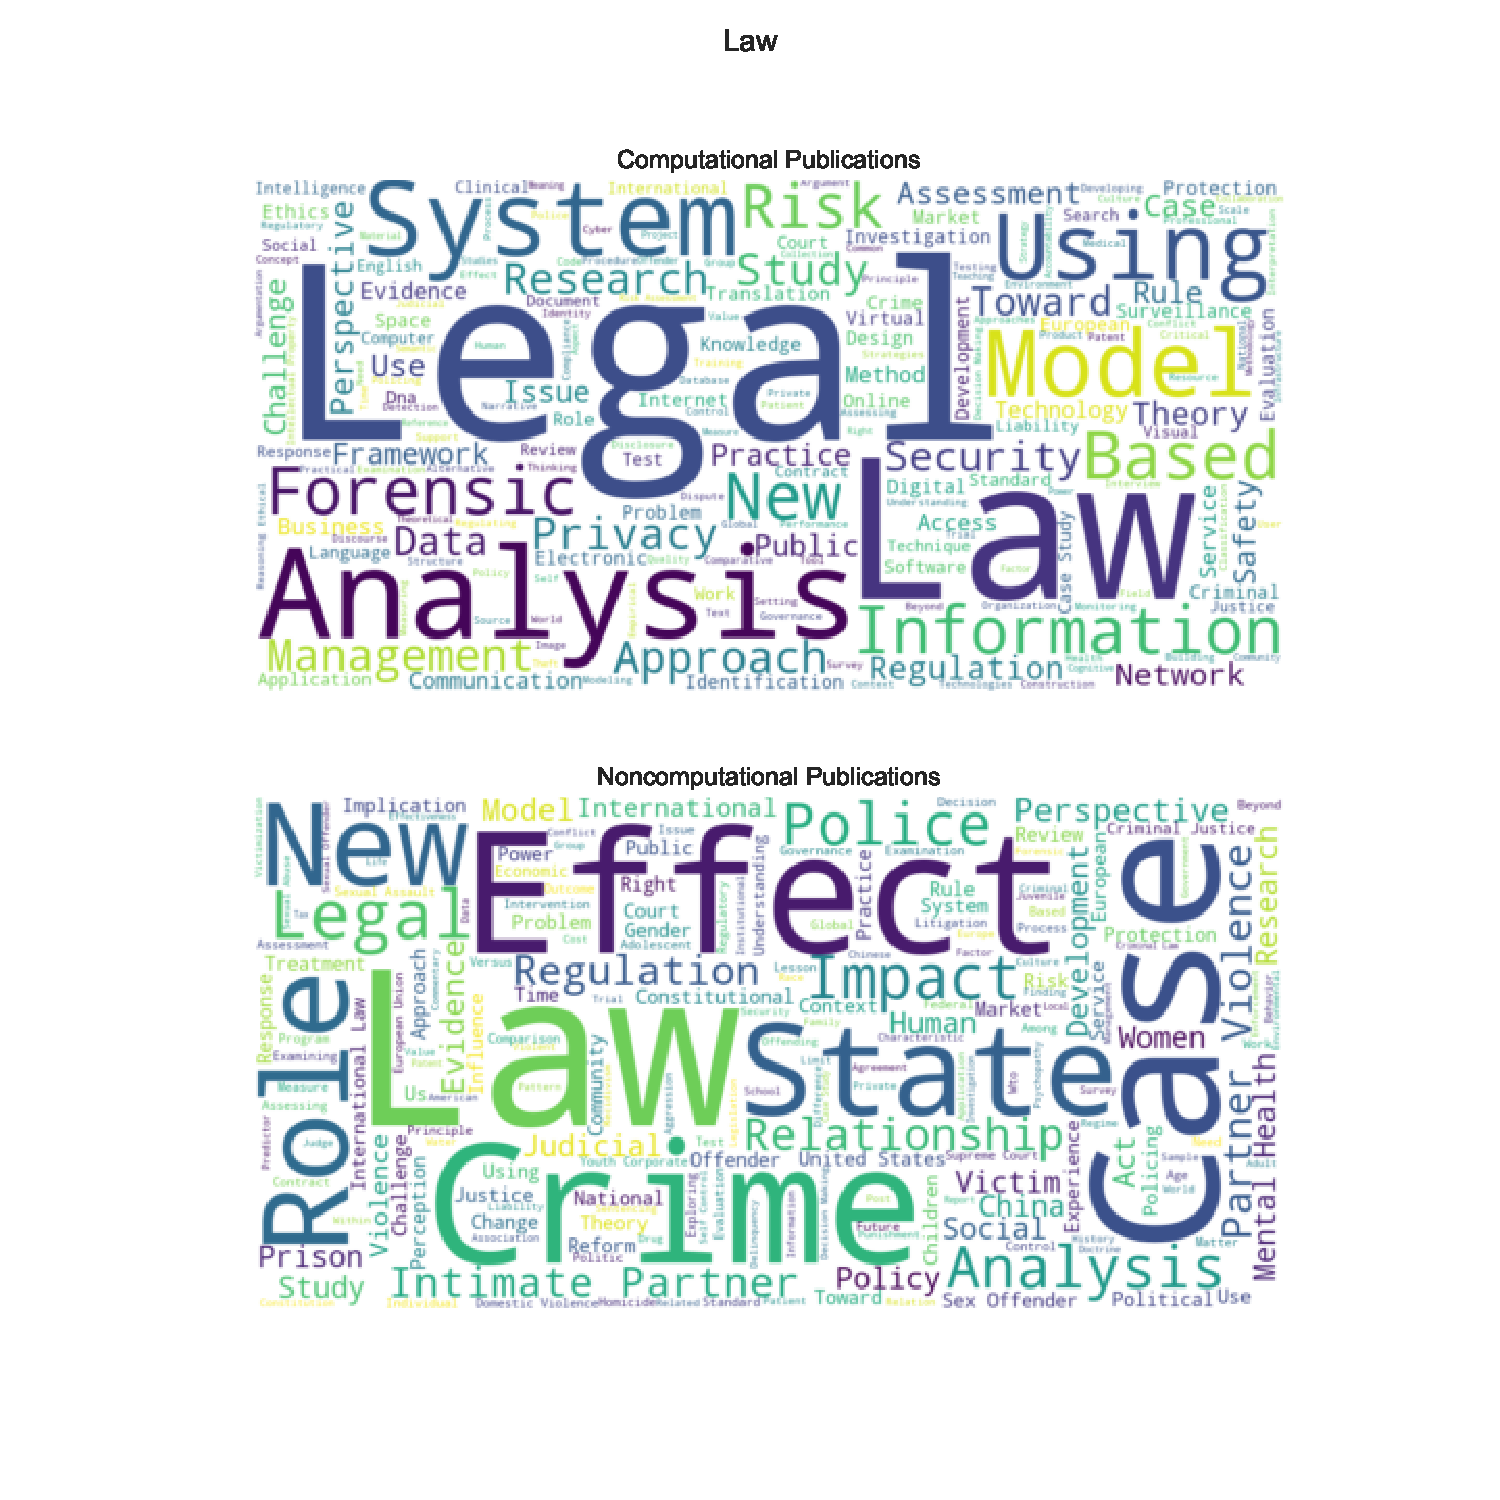
\includegraphics[width=\textwidth]{wc_Law}
	\caption{Word cloud of Law publication's titles}
\end{figure}
\section{Appendix: Word2Vec t-SNE}\label{appendix_tsne}
\begin{figure}[H]
	\centering
	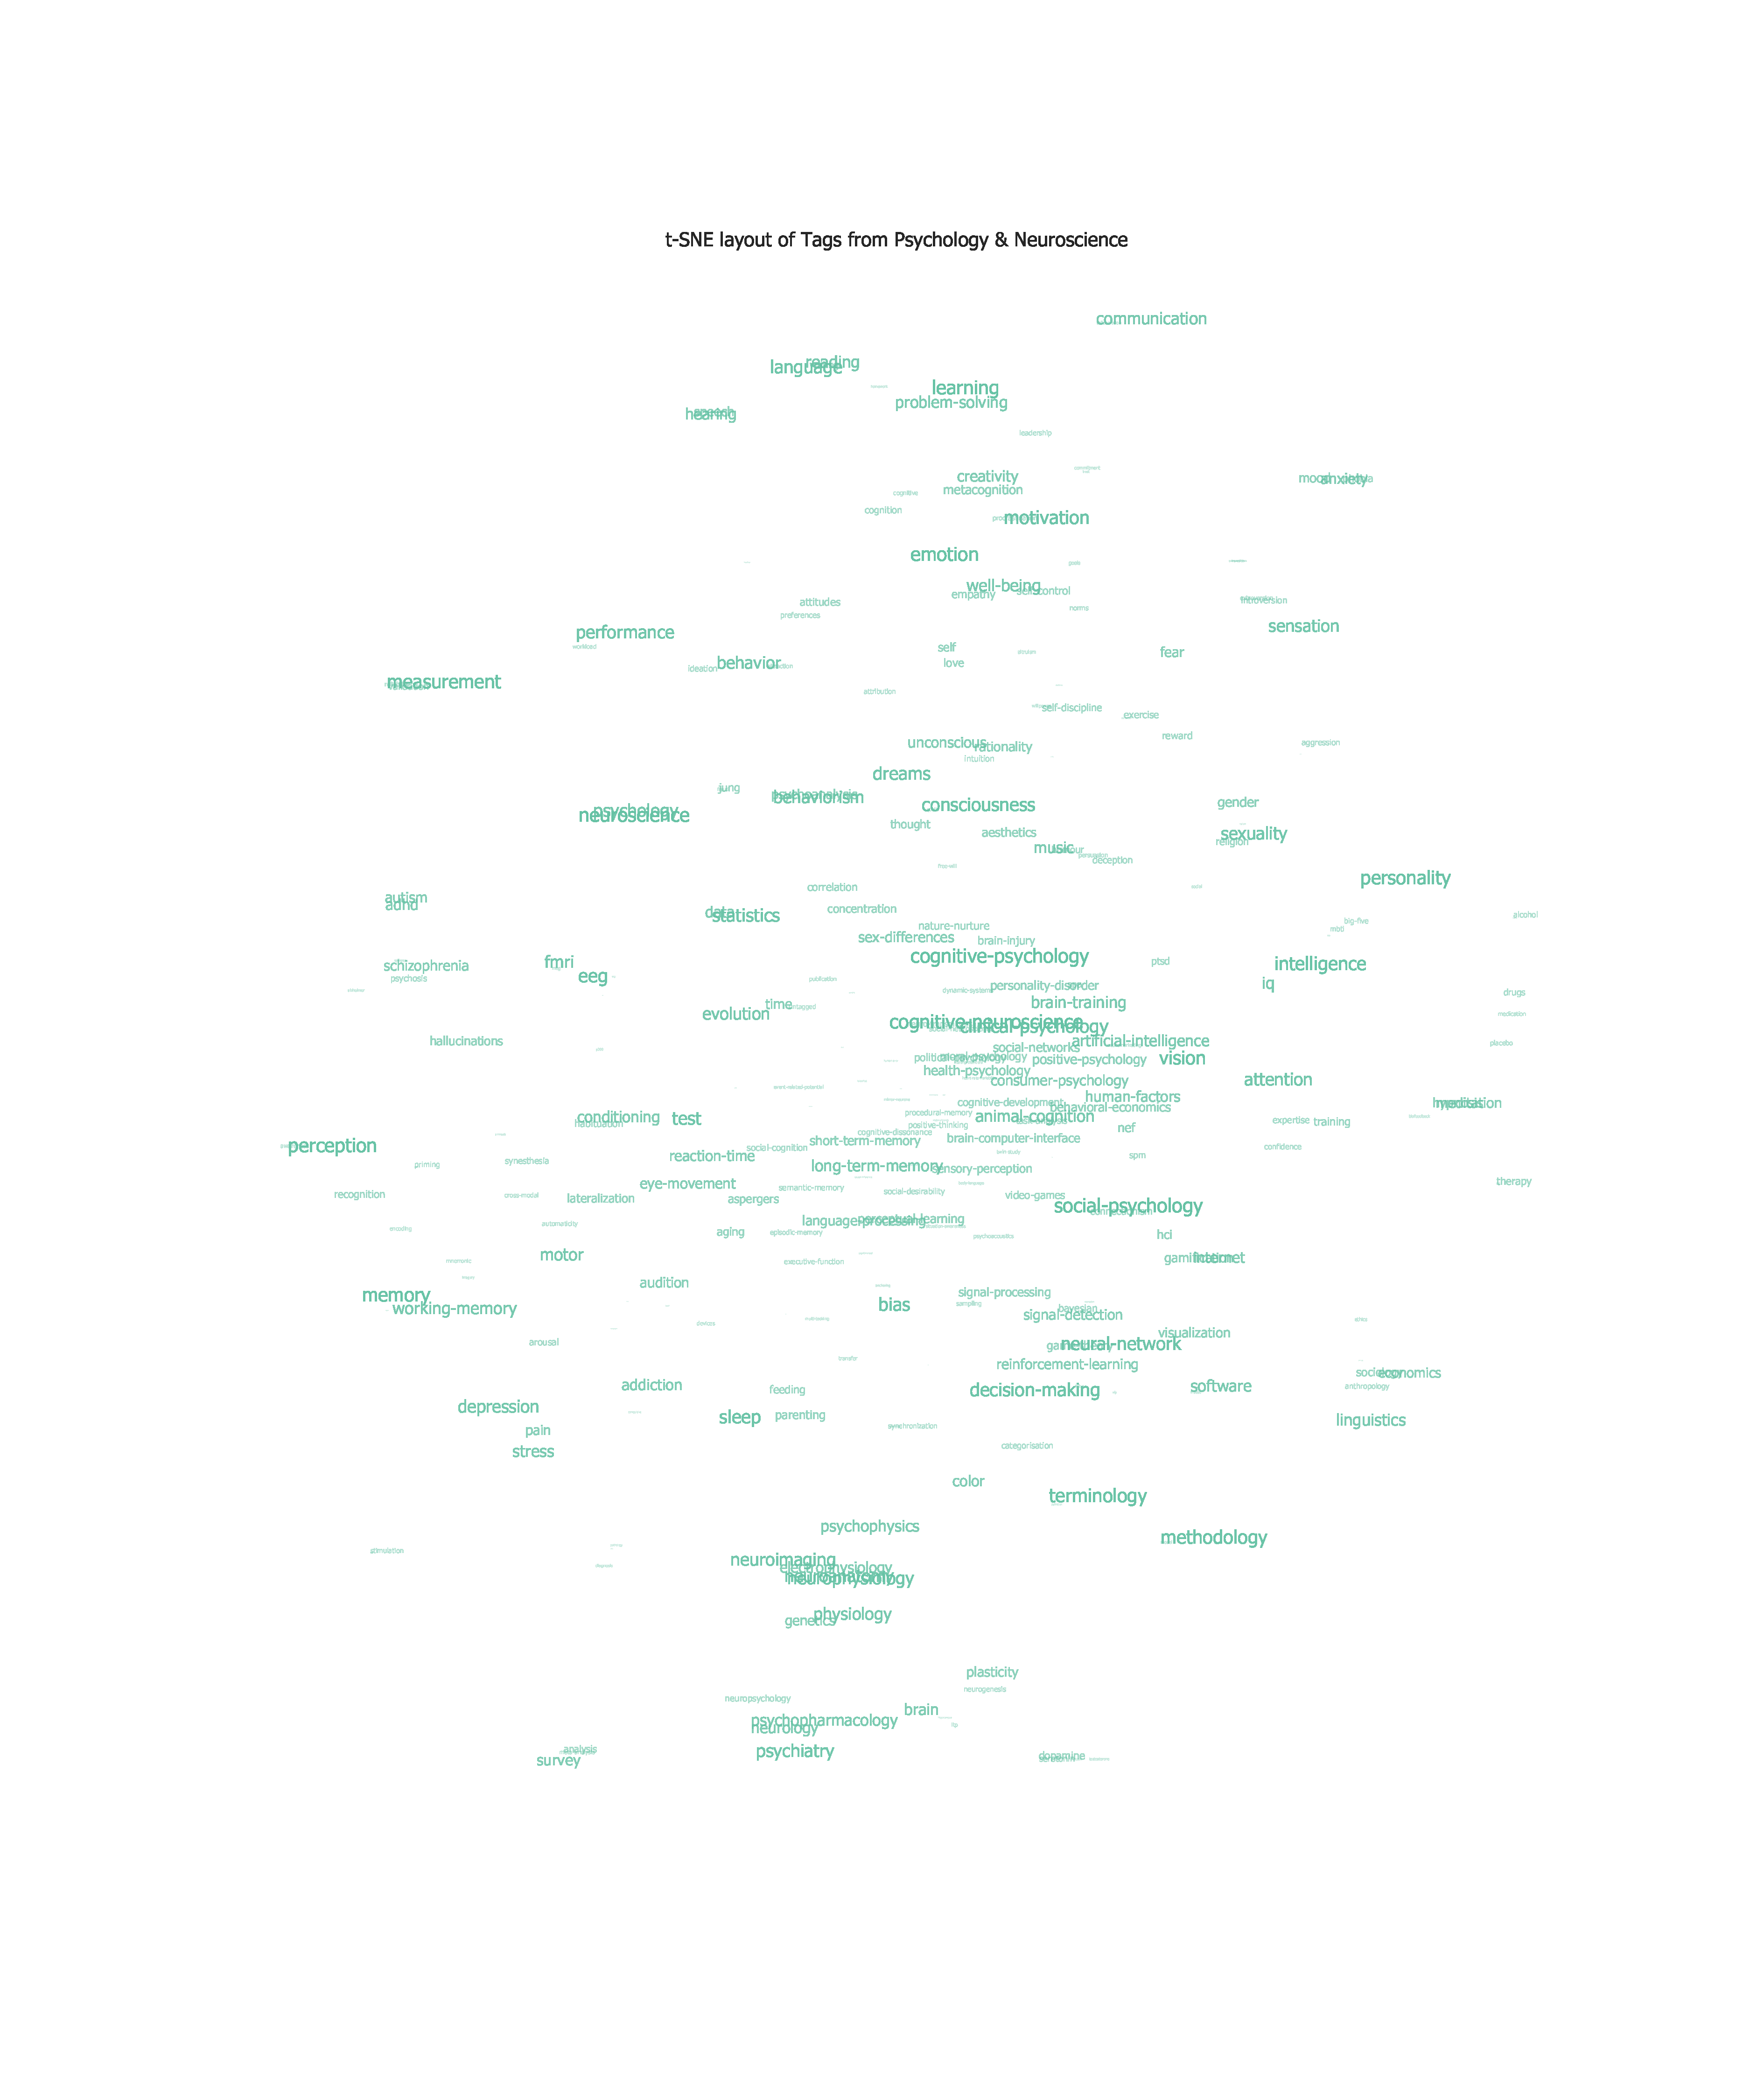
\includegraphics[height=\textheight]{tsne_psychologyneuroscience}
	\caption{t-SNE layout of Tags from Psychology \& Neuroscience}
\end{figure}
\begin{figure}[H]
	\centering
	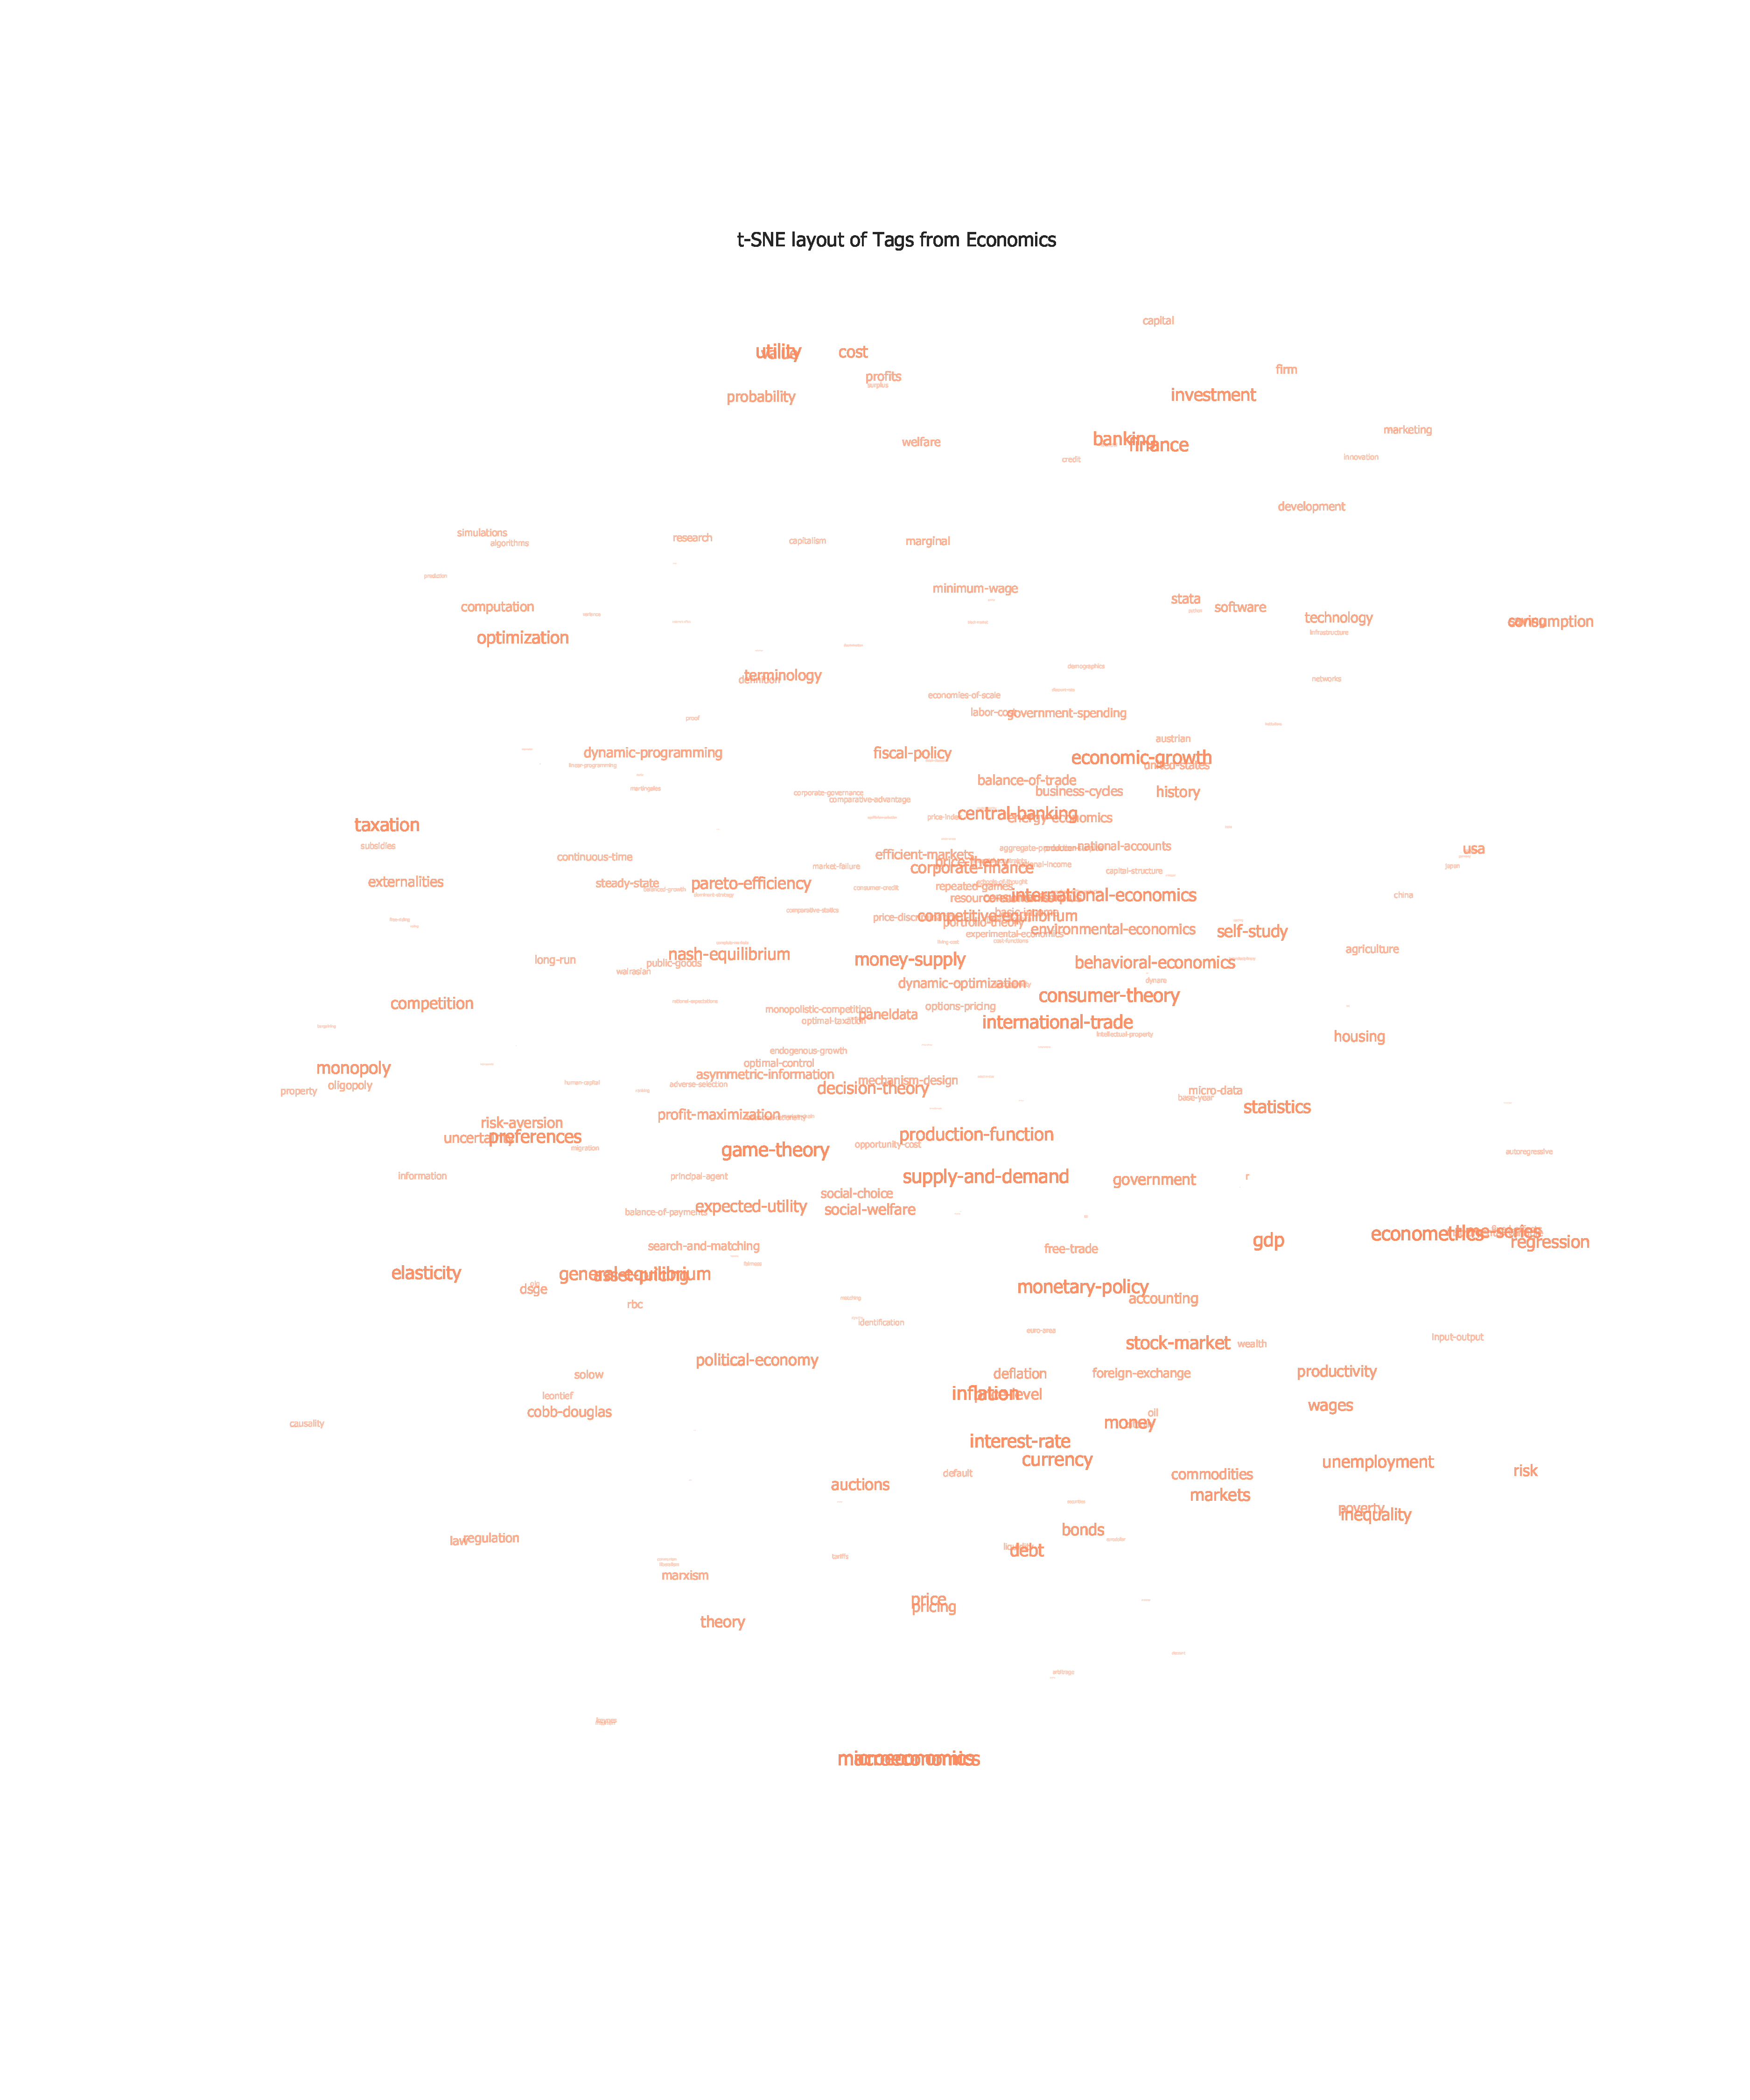
\includegraphics[height=\textheight]{tsne_economics}
	\caption{t-SNE layout of Tags from Economics}
\end{figure}
\begin{figure}[H]
	\centering
	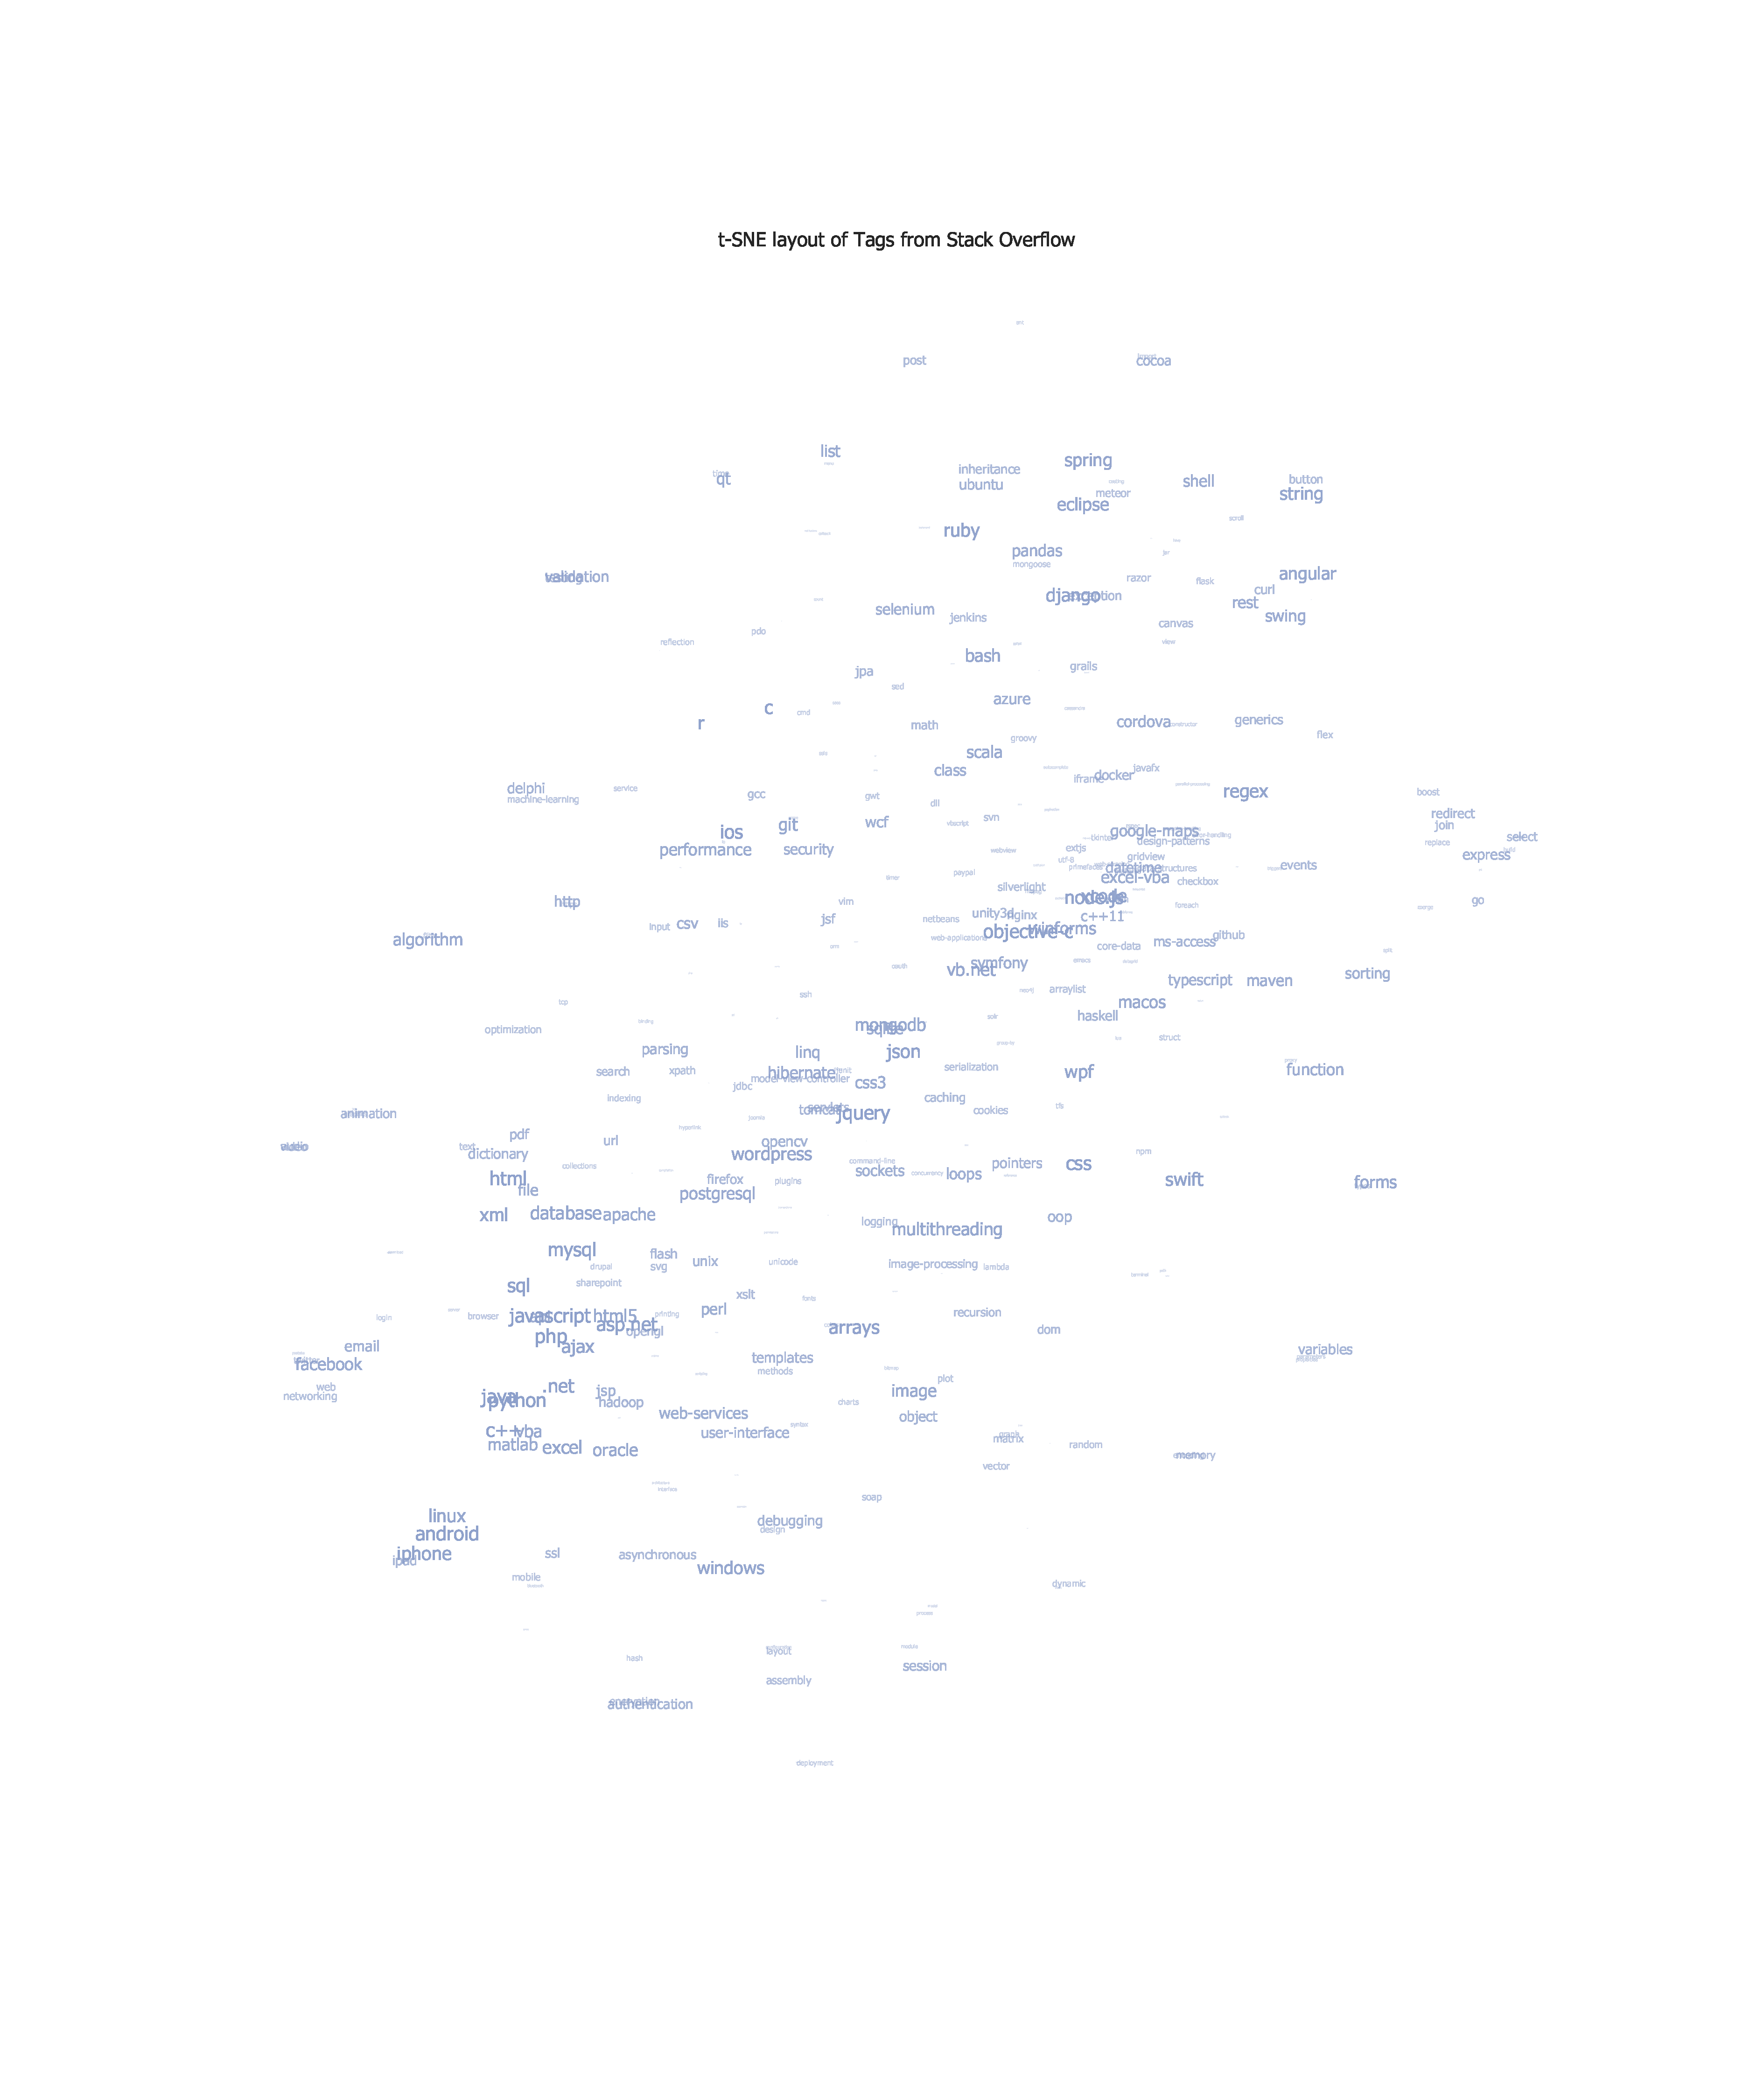
\includegraphics[height=\textheight]{tsne_stack_overflow}
	\caption{t-SNE layout of Tags from Stack Overflow}
\end{figure}
\end{document}